\documentclass[conference]{IEEEtran}
\IEEEoverridecommandlockouts
\usepackage{cite,amsmath,amssymb,amsthm,graphicx,booktabs,multirow,url,xcolor,threeparttable}
\usepackage[hidelinks]{hyperref}
\usepackage{siunitx}
\usepackage{pifont}
\usepackage[normalem]{ulem}
\usepackage{placeins}
%, float placement: allow more floats per page so none is deferred past the text
\setcounter{topnumber}{4}\setcounter{bottomnumber}{3}\setcounter{totalnumber}{6}
\setcounter{dbltopnumber}{4}
\renewcommand{\topfraction}{0.92}\renewcommand{\bottomfraction}{0.85}
\renewcommand{\textfraction}{0.06}\renewcommand{\floatpagefraction}{0.70}
\renewcommand{\dbltopfraction}{0.92}\renewcommand{\dblfloatpagefraction}{0.70}
\newcommand{\cmark}{\textcolor{green!45!black}{\ding{51}}}
\newcommand{\xmark}{\textcolor{red!70!black}{\ding{55}}}
\usepackage{tikz}
\usetikzlibrary{positioning,arrows.meta,calc,shapes.geometric,fit,backgrounds,decorations.pathmorphing}
\newtheorem{theorem}{Theorem}
\newtheorem{proposition}{Proposition}
\newtheorem{lemma}{Lemma}
\newtheorem{assumption}{Assumption}
\usepackage{amsthm}
\newtheorem{remark}{Remark}
\DeclareMathOperator*{\argmin}{arg\,min}
\DeclareMathOperator{\NB}{NegBin}
\newcommand{\bR}{\mathbb{R}}
\newcommand{\E}{\mathbb{E}}

\begin{document}

\title{RIG-Net: A Renewal--Importation Graph Network with Genomic Priors and Intervention-Aware Dynamics for Sub-national Ebola Forecasting}

\author{\IEEEauthorblockN{Author Name}
\IEEEauthorblockA{\textit{Affiliation} \\
\textit{Institution}\\
City, Country \\
email@domain}}

\maketitle

\begin{abstract}
Sub-national Ebola forecasts guide where treatment beds and contact tracers are deployed, yet the available panels are short, sparse and dominated by zeros. We present RIG-Net-GI, a graph neural network whose decoder is the epidemic renewal equation parameterised by the Ebola generation interval, so the network predicts a reproduction number, an importation share and an introduction rate rather than raw counts. Two domain priors are added: a genomic transmission-linkage graph built only from genomes sampled before each forecast origin, and an intervention-aware term driven by surveillance-derived response intensity. We prove the rollout is bounded, contractive below $\bar R=1$, and that its error growth follows the spectral radius of a renewal companion operator, then verify each claim empirically. Against 16 models published 2020--2026 on 61 West African districts and 29 Congolese health zones, under rolling-origin evaluation with 5 seeds, RIG-Net-GI ranks first of 18 on the DRC panel and fourth on West Africa, where it leads on RMSE and correlation. It emits predictive intervals no baseline provides, well calibrated on the DRC panel without post-hoc adjustment. Negative results are reported in full: a Nemenyi test cannot separate it from nine baselines, its learned reproduction number does not reproduce an EpiEstim estimator, and its West African intervals are one-sided.
\end{abstract}

\begin{IEEEkeywords}
epidemic forecasting, graph neural networks, renewal equation, genomic epidemiology, Ebola virus disease, spatio-temporal modelling
\end{IEEEkeywords}

\section{Introduction}

\IEEEPARstart{S}{ub-national} epidemic forecasting underpins high-stakes operational decisions in outbreak response. Treatment beds, vaccination rings, safe-burial teams and contact tracers are allocated to districts and health zones, not to countries, so a forecast is actionable only at that resolution and only if it arrives with enough lead time to move resources~\cite{who2014}. Ebola remains a recurring threat whose clinical and operational management continues to evolve~\cite{rojek2025}, and machine learning is now applied across every epidemiological stage of such zoonotic diseases~\cite{zhang2026}. The 2013--16 West African Ebola epidemic and the 2018--20 Nord Kivu epidemic are the two largest filovirus events on record, and both generated dense sub-national surveillance streams alongside unprecedented genomic surveillance~\cite{dudas2017,kinganda2021}. Turning those streams into regional forecasts that responders can act on remains an open problem.

\begin{figure}[t]
\centering
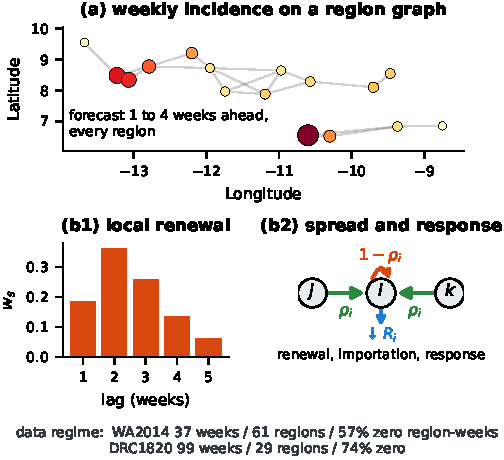
\includegraphics[width=\columnwidth]{figs/problem.pdf}
\caption{The forecasting problem. (a)~Weekly incidence on a region graph. (b1)~The Ebola generation interval $w_s$, which weights local renewal. (b2)~The three terms acting on region $i$: a share $1-\rho_i$ of its infection pressure is generated locally (orange self-loop), a share $\rho_i$ is imported from neighbours (green), and the response suppresses $R_i$ (blue). The footer gives the data regime.}
\label{fig:problem}
\end{figure}

The forecasting task is illustrated in Fig.~\ref{fig:problem}. Weekly case counts are observed on a region graph, and the model must predict each region's incidence one to four weeks ahead. Three distinct structures drive those counts. Transmission \emph{renews} locally: today's cases are generated by cases one to three weeks earlier, weighted by the pathogen's generation-interval distribution. Chains are \emph{imported} between regions, sometimes across national borders far from the origin. And transmission is \emph{suppressed} as isolation capacity, case finding and vaccination reach a region. Critically, the data regime is the opposite of the benchmarks that drive progress in spatio-temporal forecasting: an Ebola panel yields one to two years of weekly counts over a few dozen regions, 57--74\% of region-weeks contain no cases at all, and reporting backlogs occasionally exceed true weekly incidence by an order of magnitude. Where individual mobility traces exist they can be modelled directly~\cite{liu2023human}; for these outbreaks they do not, which is why we infer the spatial operator from counts and genomes instead.

Existing approaches fall into three classes, each limited in this regime. \textit{Deep temporal forecasters} such as N-BEATS~\cite{nbeats}, PatchTST~\cite{patchtst} and iTransformer~\cite{itransformer} model each series with a flexible function class but ignore the region graph, and the heavier variants are designed for long, quasi-stationary series with thousands of time steps. \textit{Spatio-temporal graph neural networks} such as AGCRN~\cite{agcrn}, MTGNN~\cite{mtgnn}, Cola-GNN~\cite{colagnn} and EpiGNN~\cite{epignn} learn an adjacency jointly with the forecast, as do the recent traffic models MAST-Net~\cite{mastnet}, CHAMFormer~\cite{chamformer} and MCPST~\cite{mcpst}, which add manifold, heterogeneous-coupling and physics-consensus constraints respectively, with related work transferring cross-city knowledge under a few-shot constraint~\cite{xcity} and addressing class imbalance in node classification~\cite{cl3an}, but map past counts directly to future counts, so their parameters carry no epidemiological meaning and their learned graphs often reduce to a smoothed distance kernel. Mechanistic models of Ebola have a long lineage, from the compartmental formulation of Legrand et al.~\cite{legrand2007}, still the basis of most Ebola simulators, to recent fractional-order treatments of vaccination control~\cite{yunus2025} and modular high-performance simulators such as MEmilio~\cite{memilio2026}. A recent review traces the field's movement from these mechanistic models toward data-driven ones~\cite{sun2026}, which is the boundary this paper works on. \textit{Mechanistic hybrids} such as MepoGNN~\cite{mepognn} couple a network to compartmental SIR dynamics, which require a population denominator and a recovery rate that are weakly identified at health-zone resolution. Section~\ref{sec:related} reviews all three.

Four challenges therefore persist for sub-national outbreak forecasting: (i)~\textit{no mechanistic grounding}, so forecasts cannot be read as statements about transmission and offer responders no interpretable quantity; (ii)~\textit{unused domain priors}, since viral genomes resolve long-range introductions that geography cannot, yet have been used only retrospectively; (iii)~\textit{no treatment of the response itself}, although intervention intensity is precisely what drives an outbreak down; and (iv)~\textit{fragile evaluation}, because a single chronological split on an epidemic panel can place the entire test period in a near-zero tail where no model is distinguishable from repeating last week.

RIG-Net-GI is distinguished from recent graph anomaly-free forecasting advances in three respects. First, unlike spatio-temporal GNNs that emit counts~\cite{mtgnn,staeformer,stid}, it emits epidemiological parameters and generates counts through the renewal equation, so every forecast carries a reproduction-number-like parameter and an importation share, whose relation to an established estimator we measure rather than assume. Second, unlike the SIR hybrid MepoGNN~\cite{mepognn}, it couples to a mechanism whose only free quantity, the generation interval, is measured for Ebola~\cite{who2014} rather than inferred. Third, unlike phylodynamic studies that use genomes to explain transmission after the fact~\cite{dudas2017,kinganda2021}, and unlike deep spatio-temporal models applied to Ebola on case and mobility streams alone~\cite{deepevd,stflam}, it uses genomes as a forecasting prior, which requires rebuilding the linkage graph at every forecast origin so that no future sequence informs a past prediction.

We propose \textit{RIG-Net-GI}, a Renewal--Importation Graph Network with genomic priors and intervention-aware dynamics, which treats a region graph as a coupled renewal process whose local reproduction number, importation share and introduction rate are predicted by a GNN. Anomalous growth is therefore expressed not as a large residual but as a reproduction number above one, and spatial spread as a share of infection pressure drawn through a learned operator. This perspective offers four advantages: (1)~a mechanistic foundation whose only fixed quantity is a measured generation interval; (2)~a set of structural read-outs, the gate weights, $\rho_i$ and the suppression coefficients, that can be inspected, with the caveat established in Section~\ref{sec:results} that the learned $R$ is a shrunk forecasting parameter and not an epidemiological estimate; (3)~a principled route to inject domain priors, because the graph operator and the reproduction number are separate inputs to the mechanism; and (4)~analysable dynamics, since the rollout is a linear recursion whose stability can be characterised exactly.

Building on this formulation, we operationalise it through four components: (i)~a \textit{multi-graph fusion} module that mixes geographic, learned, attention and genomic adjacencies with a per-region gate; (ii)~a \textit{genomic transmission-linkage prior} built only from genomes sampled before each forecast origin, with rows masked for unsequenced regions; (iii)~an \textit{intervention-aware reproduction head} that multiplies an intrinsic $R$ by a non-negative exponential suppression term on surveillance-derived response intensity; and (iv)~a \textit{renewal decoder} that rolls the resulting parameters forward four weeks under a negative-binomial likelihood. Fig.~\ref{fig:arch} gives the overview.

\textbf{Contributions.} The main contributions of this work are:
\begin{itemize}
    \item \textit{Renewal-equation decoder for GNNs}: we make the epidemic renewal equation, carrying the measured Ebola generation interval, a differentiable decoder whose parameters a graph network predicts, yielding an interpretable and autoregressive multi-step forecast.
    \item \textit{Leakage-safe genomic and intervention priors}: we construct a transmission-linkage graph from 1{,}610 Makona and 852 Nord Kivu genomes, recomputed at every forecast origin, and a monotone intervention-suppression term fitted by projected gradient descent; we show genomic linkage is \emph{negatively} correlated with distance and so supplies information a distance kernel cannot.
    \item \textit{Theory with empirical validation}: we prove boundedness, contraction below $\bar R=1$, an $H$-step error bound governed by the spectral radius of a renewal companion matrix, a Lipschitz bound for multi-graph fusion, and identifiability conditions for the importation share, then verify all three behavioural claims directly on the forecasts.
    \item \textit{A rigorous four-country benchmark}: fifteen models published 2020--2026 are compared across 61 districts of Guinea, Liberia and Sierra Leone and 29 health zones of North Kivu, Ituri and South Kivu, under a rolling-origin protocol spanning growth, peak, decline and tail, with equal budgets, five seeds and 1{,}446 training runs, and with model selection fixed on validation data before any test result was read.
\end{itemize}

We report positive and negative findings alike. RIG-Net-GI attains the lowest error of all nineteen systems on the DRC panel and the best RMSE, correlation and sMAPE on West Africa, with calibrated predictive intervals; but it ranks fourth by MAE there, is statistically tied with nine baselines once multiple comparisons are corrected, is the worst learned model at timing local peaks, and its intervention term helps on only one of the two panels. We trace each failure to a mechanism our theory predicts.

The remainder of this paper is organised as follows. Section~\ref{sec:related} reviews related work in epidemic forecasting, spatio-temporal graph learning and genomic epidemiology. Section~\ref{sec:prelim} introduces the problem formulation and renewal-equation preliminaries. Section~\ref{sec:method} details the proposed framework, Section~\ref{sec:theory} develops its theoretical analysis with proofs, Section~\ref{sec:setup} describes the benchmark and protocol, Section~\ref{sec:results} reports experimental results across fourteen research questions, Section~\ref{sec:analysis} discusses implications and threats to validity, and Section~\ref{sec:conclusion} concludes.

\section{Related work}\label{sec:related}

\subsection{Deep multivariate forecasting}

A line of work argues that carefully regularised, architecturally simple models match or beat transformers on multivariate series. N-BEATS~\cite{nbeats} and N-HiTS~\cite{nhits} stack residual MLP blocks with backcast/forecast decomposition; DLinear~\cite{dlinear} reduces forecasting to two linear maps on a trend/remainder split and questions whether attention helps at all; TSMixer~\cite{tsmixer} alternates time- and feature-mixing MLPs. Against these, Autoformer~\cite{autoformer} introduces series decomposition with FFT auto-correlation, PatchTST~\cite{patchtst} treats a series as patches with channel independence and reversible instance normalisation, TimesNet~\cite{timesnet} folds FFT-selected periods into 2-D convolutions, and iTransformer~\cite{itransformer} inverts the attention axis so that variates rather than time steps are tokens. These models are evaluated almost exclusively on long, densely sampled, quasi-stationary benchmarks (traffic, electricity, weather) with thousands of time steps. Our panels have 37 and 99 weeks and 57--74\% zeros, and our results reproduce the simplicity finding in that regime: N-BEATS and N-HiTS are among the strongest baselines, while TimesNet, Autoformer and TSMixer fall below a naive forecast on at least one panel.

\subsection{Spatio-temporal graph neural networks}

Where regions interact, graph structure is the natural inductive bias. AGCRN~\cite{agcrn} learns node-adaptive parameters and an adjacency from node embeddings inside a GRU; MTGNN~\cite{mtgnn} learns a sparse directed graph jointly with dilated temporal convolutions and mix-hop propagation; STID~\cite{stid} shows much of the benefit can be recovered with spatial and temporal identity embeddings plus an MLP; STAEformer~\cite{staeformer} adds an adaptive spatio-temporal embedding to a vanilla transformer. A recurring question in this literature is whether the learned graph encodes anything beyond a smoothed distance kernel. Our gating analysis speaks to this directly: the learned and attention channels together receive only 24\% of the mixing weight on WA2014, against 47\% for the fixed geographic kernel and 28\% for the genomic graph, and the genomic channel is shown to be \emph{negatively} correlated with distance, so it is the externally supplied prior rather than the learned structure that adds the long-range information.

\subsection{Epidemic-specific graph models}

Epidemiological GNNs add domain structure to the above. Cola-GNN~\cite{colagnn} combines cross-location attention with a geographic adjacency through a learned gate, an idea our fusion generalises to four channels. EpiGNN~\cite{epignn} encodes local and global transmission risk and a region-aware graph learner. MepoGNN~\cite{mepognn} is the closest prior work in spirit: it couples a spatio-temporal network to a metapopulation SIR model with a learned mobility graph, so that the network predicts epidemiological parameters rather than counts. Our decoder differs in the mechanism it couples to. SIR compartments require a population denominator and a recovery rate, which are weakly identified for Ebola at health-zone resolution; empirically MepoGNN is the weakest graph baseline on both our panels. The renewal equation instead requires only the generation-interval distribution, which for Ebola is measured~\cite{who2014}, and it is the estimating equation already used in outbreak response.

\subsection{Renewal-equation estimation}

The renewal formulation~\cite{fraser2007} and its practical estimator EpiEstim~\cite{cori2013} are standard for estimating a time-varying reproduction number, and metapopulation extensions couple regions through mobility~\cite{riley2007}. This literature is estimation-oriented: $R_t$ is inferred retrospectively from observed incidence under a fixed generation interval, usually without a learned spatial operator and without multi-step forecasting. We invert the usual arrangement by making the renewal equation a differentiable \emph{decoder} whose parameters are predicted by a GNN, which keeps the interpretability of $R_t$ while producing autoregressive multi-week forecasts. The price, as our theory and experiments both show, is that the decoder inherits the renewal equation's momentum: it contracts when $\bar R<1$ and amplifies when $\bar R>1$.

\subsection{Genomic epidemiology}

Phylodynamic analysis of the 2013--16 West African epidemic~\cite{dudas2017} reconstructed the spread of 1{,}610 Makona genomes and identified cross-border introductions and the role of mobility and administrative boundaries; genomic surveillance was integrated into the Nord Kivu response in near-real time with 792 genomes analysed as they were generated~\cite{kinganda2021}. These studies use genomes to explain transmission retrospectively. The enabling capability is portable real-time sequencing, demonstrated during the West African epidemic itself~\cite{quick2016} and since generalised into routine outbreak genomic surveillance~\cite{grubaugh2019}, with open platforms such as Nextstrain making lineage information available while an outbreak is still running~\cite{hadfield2018}. That these data now arrive in near-real time is precisely what makes a forecasting prior conceivable; what remains missing is a model that consumes them prospectively. To our knowledge genomes have not previously been used as a \emph{forecasting} prior, and doing so raises a leakage problem absent from retrospective work: a phylogeny estimated from the full data set encodes the future. We therefore rebuild the linkage graph at every forecast origin from genomes sampled strictly before it, and report how sequencing breadth across regions, rather than depth, determines how much of that graph is usable.

\subsection{Evaluation practice}

Forecasting comparisons are sensitive to protocol. The predictive median is the Bayes act under absolute loss~\cite{gneiting2011}, a point our ablations confirm is worth 12--13\% of validation MAE on these counts, and proper scoring of the predictive distribution is standard in collaborative epidemic forecasting, where the weighted interval score has become the common currency~\cite{bracher2021} and large multi-team evaluations have shown how much conclusions depend on the scoring protocol~\cite{cramer2022}. Pairwise significance in this setting is conventionally assessed with the Diebold--Mariano test~\cite{diebold1995}, which we use alongside a rank-based correction. Much of the spatio-temporal GNN literature reports a single chronological split, which on an epidemic panel can place the entire test period in a near-zero tail; our rolling-origin protocol with phase-labelled blocks is designed to avoid that, and our measured validation-to-test rank correlation of 0.72 on WA2014 quantifies how badly a single split can mislead.


\section{Preliminaries}\label{sec:prelim}

\subsection{Problem setting}

Let $\mathcal{V}=\{1,\dots,N\}$ index regions and $t=1,\dots,T$ index epidemiological weeks. Let $y_i(t)\in\mathbb{Z}_{\geq0}$ denote new cases reported in region $i$ during week $t$, and write $\mathbf{y}(t)\in\mathbb{Z}_{\geq0}^N$. Given a lookback window of length $L$ and a horizon $H$, a forecaster issued at origin $t$ observes $\mathbf{Y}_{t}=[\mathbf{y}(t-L),\dots,\mathbf{y}(t-1)]$ together with static covariates $\mathbf{S}\in\bR^{N\times d_S}$ and side information available strictly before $t$, and predicts $\hat{\mathbf{y}}(t),\dots,\hat{\mathbf{y}}(t+H-1)$. We use $L=6$, $H=4$.

\subsection{The renewal equation}

The renewal (Lotka--Euler) formulation of epidemic dynamics~\cite{fraser2007,cori2013} states that expected incidence at time $t$ is the product of a reproduction number and the infection pressure generated by past cases weighted by the generation-interval distribution $w$:
\begin{equation}
\E[y_i(t)] \;=\; R_i(t)\sum_{s\geq1} w_s\, y_i(t-s).
\label{eq:renewal}
\end{equation}
Here $w_s\geq0$, $\sum_s w_s=1$, and $w$ is a property of the pathogen rather than a free parameter. For Ebola virus disease, the generation interval is well characterised: the WHO Ebola Response Team estimated a mean of \SI{15.3}{days} with standard deviation \SI{9.3}{days}~\cite{who2014}. Discretising the corresponding gamma density to weekly bins over lags $1,\dots,5$ gives
\begin{equation}
w = (0.185,\,0.361,\,0.258,\,0.135,\,0.061).
\label{eq:w}
\end{equation}
Equation~\eqref{eq:renewal} is the estimating equation behind EpiEstim~\cite{cori2013} and is standard in outbreak analytics; our contribution is to use it as a \emph{decoder} for a neural network rather than as a standalone estimator.

\subsection{Spatial coupling and importation}

Equation~\eqref{eq:renewal} is purely local. Cross-region transmission is introduced by letting a fraction $\rho_i\in[0,1]$ of the infection pressure driving region $i$ originate elsewhere, distributed according to a row-stochastic matrix $A$:
\begin{equation}
\begin{aligned}
Q_i(t) &= (1-\rho_i)\,P_i(t) \;+\; \rho_i \sum_{j} A_{ij}\,P_j(t),\\[2pt]
P_i(t) &= \sum_{s=1}^{G} w_s\, y_i(t-s).
\end{aligned}
\label{eq:import}
\end{equation}
This is the discrete-time analogue of a metapopulation force of infection~\cite{riley2007} with the mobility kernel replaced by a learned operator.

\subsection{Counting distribution}

Ebola region-weeks are zero-inflated and over-dispersed: the variance of weekly incidence exceeds its mean by a factor of 20--60 in both panels. We therefore model $y_i(t)\sim\NB(\mu_i(t),\alpha_i)$ with mean $\mu$ and dispersion $\alpha_i>0$, so $\mathrm{Var}=\mu+\alpha_i\mu^2$. Because the evaluation metric is MAE, point forecasts are the predictive \emph{median}, which is the Bayes act under absolute loss~\cite{gneiting2011}; this choice alone reduced validation MAE by 12--13\% relative to the predictive mean.

\subsection{Notation for graphs}

We write $A^{\mathrm{geo}}$ for a fixed geographic kernel, $A^{\mathrm{adp}}$ for a learned static adjacency, $A^{\mathrm{dyn}}$ for a state-dependent attention adjacency and $A^{\mathrm{gen}}$ for the genomic transmission-linkage graph of Section~\ref{sec:genomic}. All are row-stochastic with zero diagonal. $\|\cdot\|_1$ denotes the induced $1$-norm and $\sigma(\cdot)$ the logistic function.


\section{Method}\label{sec:method}

Fig.~\ref{fig:arch} gives the four-component overview; Figs.~\ref{fig:fusion} and~\ref{fig:rollout} detail the two novel components.

\begin{figure*}[t]
\centering
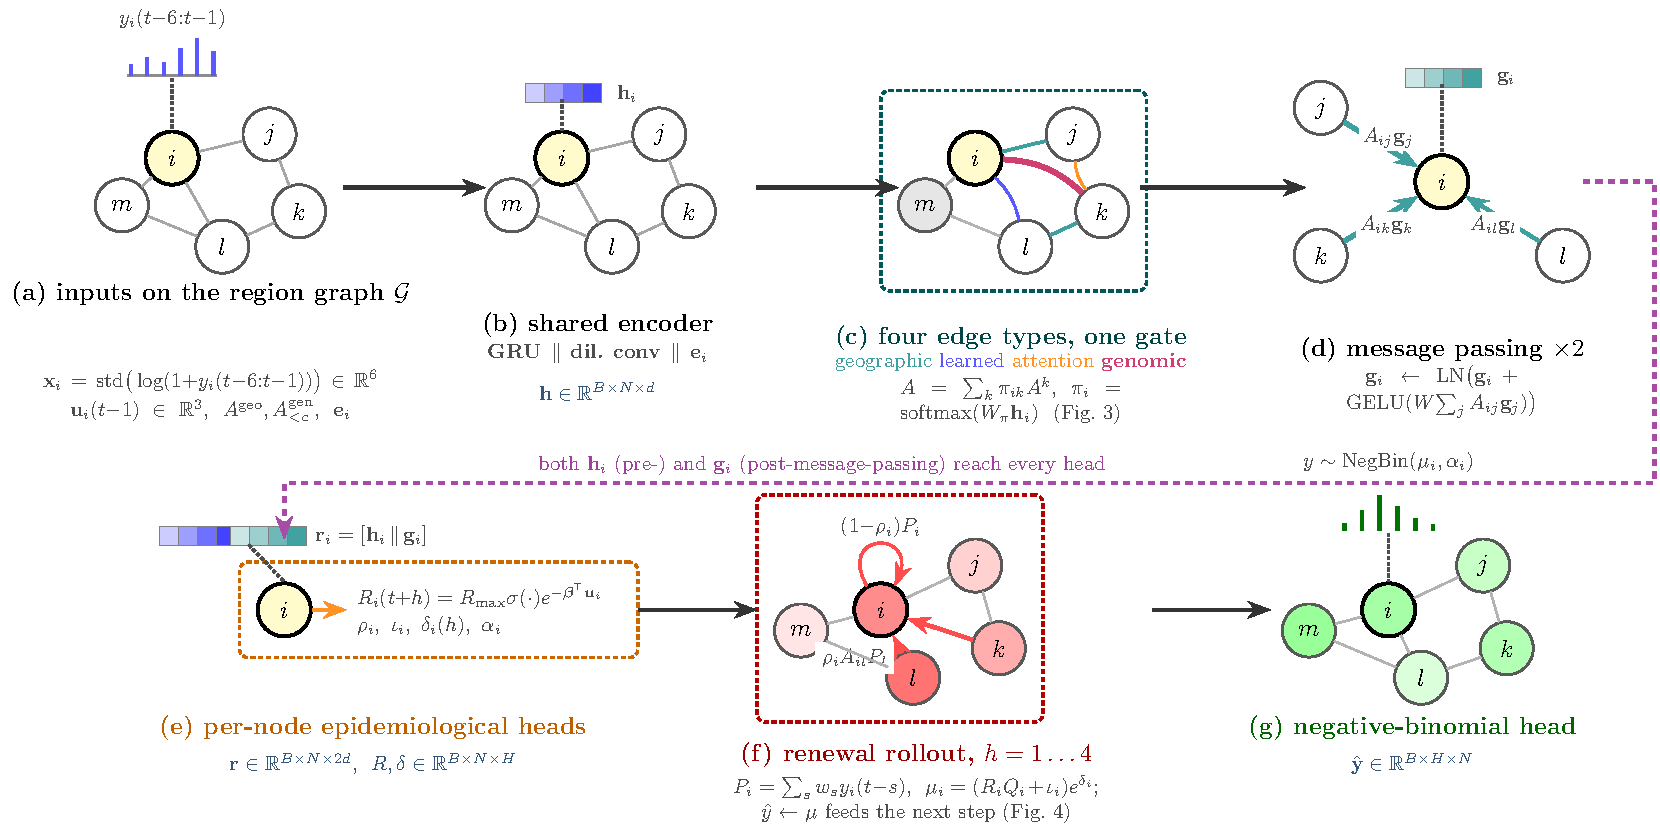
\includegraphics[width=\textwidth]{figs/arch.pdf}
\caption{RIG-Net-GI as a graph neural network; dashed boxes, each in the colour of its heading, mark the three components that are new in this work. The same five regions carry every stage. (a)~Each node holds six weeks of counts. (b)~A shared encoder turns each node's series into a state $\mathbf{h}_i$. (c)~Four edge types over the same nodes, geographic, learned, attention and the genomic transmission-linkage graph, are mixed by a per-node gate into one row-stochastic $A$; node $m$ is grey because it has no sequenced cases and its genomic row is masked. (d)~Two message-passing layers aggregate neighbour states along $A$ to give $\mathbf{g}_i$. (e)~Every head reads the concatenation $[\mathbf{h}_i\|\mathbf{g}_i]$, so the epidemiological parameters see both the node's own history and its neighbourhood. (f)~The renewal rollout turns them into four weekly means, with a share $\rho_i$ of each node's infection pressure drawn from its neighbours and the rest from itself. (g)~A negative-binomial head gives a predictive distribution at every node.}
\label{fig:arch}
\end{figure*}

\subsection{Inputs}

The model sees four things at each forecast origin $t$, all shown in Fig.~\ref{fig:arch}(a). Each region carries a six-week window of weekly confirmed-and-probable case counts, standardised as $\mathbf{x}_i=\mathrm{std}(\log(1+y_i(t{-}6{:}t{-}1)))$ with the scaler fitted on that fold's training weeks only. Each region also carries three surveillance-derived response indicators $\mathbf{u}_i(t{-}1)\in\mathbb{R}^3$ measured at the week before the origin, defined in Section~\ref{sec:interv}. Two adjacencies are fixed: the geographic kernel $A^{\mathrm{geo}}$ over seat-town coordinates, and the genomic transmission-linkage graph $A^{\mathrm{gen}}_{<c}$ rebuilt from genomes sampled strictly before that fold's cut-off $c$. Finally, each region has a free node embedding $\mathbf{e}_i$. The panels themselves, 61 West African districts over 2014--15 and 29 Congolese health zones over 2018--20, are described in Section~\ref{sec:setup}.

\subsection{Encoder and multi-graph fusion}

\textbf{Purpose.} To let each region decide for itself how much of its transmission is explained by proximity, by a learned affinity, by its current state, and by observed viral lineage sharing, instead of committing the whole panel to one notion of adjacency.

\textbf{Novelty.} Gated fusion of two adjacencies is established~\cite{colagnn}; we extend it to four channels and add a channel carried by external evidence rather than learned from the counts. The gate is masked per region, so a region with no sequenced cases renormalises over the remaining three channels rather than being given an imputed genomic row. Lemma~\ref{lem:lip} shows this extension cannot increase the Lipschitz constant of the message-passing operator, which is what makes a sparse, partially observed channel safe to add.


Each region's standardised log-incidence window $\mathbf{x}_i=\log(1+\mathbf{y}_i)$ is encoded by a GRU and a dilated causal convolution, concatenated with a node embedding $\mathbf{e}_i$ formed from a free vector plus a linear map of standardised coordinates and static covariates:
\begin{equation}
\mathbf{h}_i = W\big[\,\mathrm{GRU}(\mathbf{x}_i)\;\|\;\mathrm{Conv}(\mathbf{x}_i)\;\|\;\mathbf{e}_i\,\big].
\end{equation}
Four adjacencies are mixed by a per-region softmax gate $\pi_i=\mathrm{softmax}(W_\pi\mathbf{h}_i)\in\Delta^3$:
\begin{equation}
A = \sum_{k\in\{\mathrm{geo,adp,dyn,gen}\}} \pi_{ik}\,A^{k},
\label{eq:fuse}
\end{equation}
where $A^{\mathrm{adp}}=\mathrm{softmax}(\mathrm{ReLU}(E_1E_2^\top))$ as in~\cite{agcrn,mtgnn} and $A^{\mathrm{dyn}}=\mathrm{softmax}(q(\mathbf{h})k(\mathbf{h})^\top/\sqrt{d})$ as in~\cite{colagnn}. The genomic channel is masked out for regions with no sequenced genomes before the forecast origin, so that $\pi_{i,\mathrm{gen}}=0$ there and the remaining three weights renormalise. Two residual message-passing layers $\mathbf{g}\leftarrow\mathrm{LN}(\mathbf{g}+\mathrm{GELU}(W A\mathbf{g}))$ produce the spatial representation. Fig.~\ref{fig:fusion} draws the four adjacencies over a common region set and the gating that fuses them.

\begin{figure*}[t]
\centering
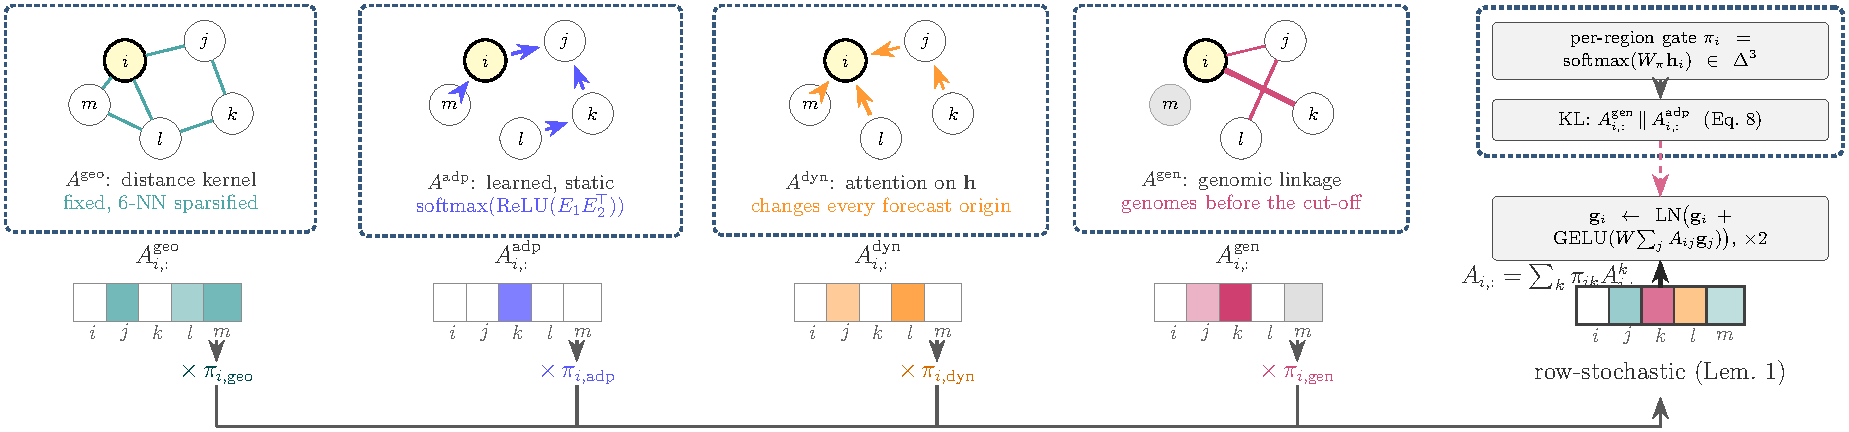
\includegraphics[width=\textwidth]{figs/fusion.pdf}
\caption{Component~1 of Fig.~\ref{fig:arch}: multi-graph fusion, shown for one focal region $i$ (shaded). Top: the same five regions carry four adjacencies, a fixed distance kernel, a learned static graph, a state-dependent attention graph, and the genomic transmission-linkage graph, whose edge widths are proportional to the number of near-identical genome pairs. Bottom: row $i$ of each adjacency, shaded by weight, is scaled by that region's gate coefficient $\pi_{ik}$ and summed into a single row-stochastic row. The genomic row is masked where a region has no sequenced cases ($m$), and the gate renormalises over the remaining channels.}
\label{fig:fusion}
\end{figure*}

\subsection{Genomic transmission-linkage prior}\label{sec:genomic}

\textbf{Purpose.} To supply the long-range links that a distance kernel cannot represent, the cross-border introductions that drove the West African epidemic, from evidence that is independent of the case counts being forecast.

\textbf{Novelty.} Genomes have been used to reconstruct Ebola spread retrospectively~\cite{dudas2017,kinganda2021}; to our knowledge they have not been used as a forecasting prior. Doing so raises a problem absent from retrospective work: a phylogeny estimated from the full data set encodes the future. We therefore rebuild the linkage graph at every forecast origin from genomes sampled strictly before it, normalise by $\sqrt{n_in_j}$ to remove the first-order effect of unequal sequencing effort, and mask unsequenced regions. Section~\ref{sec:results} shows the resulting edges are \emph{negatively} correlated with distance, so the channel is not a restatement of geography.


Let $\mathcal{G}_{<c}$ be the set of viral genomes with collection date earlier than a cut-off $c$, each annotated with the region of the sampled case. For genomes $a,b$ let $d(a,b)$ be the number of single-nucleotide differences computed over variable sites called in both sequences. Two genomes are \emph{linked} if $d(a,b)\leq\tau$ (we use $\tau=2$, i.e.\ within the typical EBOV substitution accumulation over one to two serial intervals). Writing $n_i$ for the number of genomes from region $i$,
\begin{equation}
G_{ij} \;=\; \frac{1}{\sqrt{n_i n_j}}\sum_{a\in i}\sum_{b\in j}\mathbf{1}\{d(a,b)\leq\tau\},\quad i\neq j,
\label{eq:gen}
\end{equation}
with $G_{ii}=0$. The normalisation by $\sqrt{n_in_j}$ removes the first-order effect of unequal sequencing effort, which is proportional to case counts in both outbreaks~\cite{kinganda2021}. We set $A^{\mathrm{gen}}=\mathrm{rownorm}(\log(1+G))$; the logarithm damps the heavy tail created by densely sampled epicentres.

\textbf{Leakage safety.} $A^{\mathrm{gen}}$ is recomputed for every rolling-origin fold using only $\mathcal{G}_{<c}$ with $c$ the last week of that fold's training period. No genome sampled during or after the validation or test block enters any graph used to forecast it.

\textbf{Genomic consistency regulariser.} Because $A^{\mathrm{adp}}$ and $A^{\mathrm{gen}}$ both claim to describe transmission linkage, we add a KL term pulling the learned graph toward the genomic one on the subset $\mathcal{M}$ of regions with genomes:
\begin{equation}
\mathcal{L}_{\mathrm{gen}} = \frac{\lambda}{|\mathcal{M}|}\sum_{i\in\mathcal{M}} \mathrm{KL}\!\left(A^{\mathrm{gen}}_{i\cdot}\,\|\,A^{\mathrm{adp}}_{i\cdot}\right).
\label{eq:kl}
\end{equation}

\subsection{Intervention-aware transmission}\label{sec:interv}

\textbf{Purpose.} To separate the transmission a region would sustain on its own from the suppression produced by testing, case-finding and an established response, so that the reproduction number the model reports is not silently absorbing the effect of the response.

\textbf{Novelty.} Compartmental hybrids let response effects enter implicitly through fitted parameters. We instead make suppression an explicit, signed and monotone factor: $R$ is multiplied by $\exp(-\boldsymbol{\beta}^{\top}\mathbf{u})$ with $\boldsymbol{\beta}\geq\mathbf{0}$ enforced by projected gradient descent, so each coefficient is interpretable as the multiplicative reduction in $R$ per standard deviation of that indicator and cannot change sign to improve fit. The constraint is enforced by projection rather than a softplus reparameterisation, which we found pins $\boldsymbol{\beta}$ at its initialisation (Section~\ref{sec:results}).


Direct intervention logs (vaccination rings, treatment-centre openings) are not available at weekly region resolution for either outbreak. We instead derive three weekly \emph{response-intensity} proxies $\mathbf{u}_i(t)\in\bR^3$ from the surveillance stream itself: (i) the laboratory-confirmation share $\mathrm{conf}/(\mathrm{conf}+\mathrm{prob})$, which rises as testing and isolation capacity reaches a region; (ii) the surveillance load $\log(1+\text{suspected})-\log(1+\text{cases in last 3 weeks})$, a measure of case-finding effort per true case; and (iii) response maturity $\log(1+\text{weeks since first case})$. All are standardised on training weeks only and are read at week $t-1$ for an origin at $t$, so they are strictly observable at forecast time.

The intrinsic reproduction number $\tilde R_i$ emitted by the network is modulated multiplicatively:
\begin{equation}
R_i(t+h) \;=\; \tilde R_i(t+h)\,\exp\!\big(-\boldsymbol{\beta}^\top \mathbf{u}_i(t-1)\big),\qquad \boldsymbol{\beta}\geq\mathbf{0}.
\label{eq:interv}
\end{equation}
Under the non-negativity constraint $\beta_k$ is directly interpretable: a one-standard-deviation increase in indicator $k$ multiplies $R$ by $e^{-\beta_k}$.

\begin{figure*}[t]
\centering
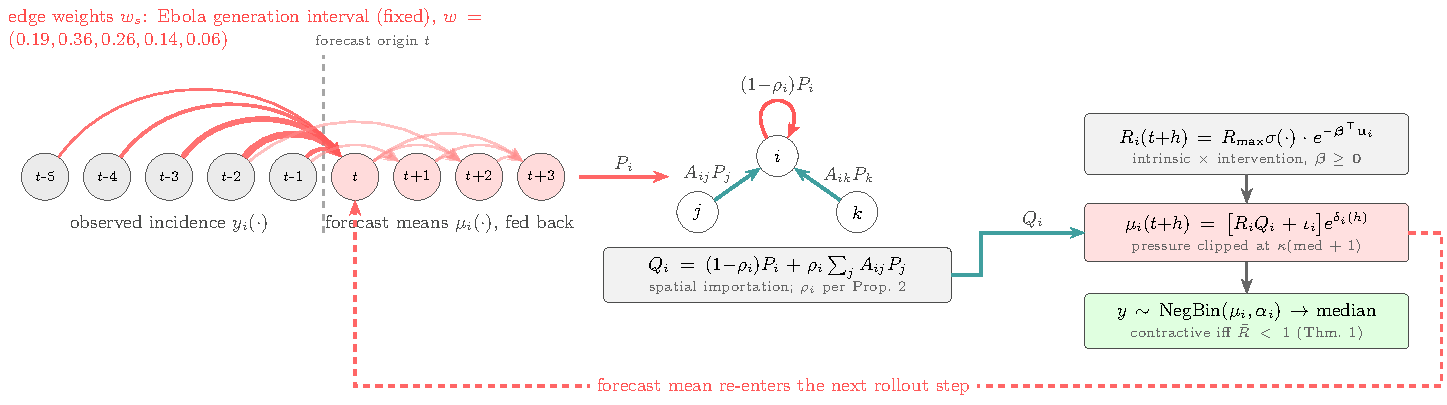
\includegraphics[width=\textwidth]{figs/rollout.pdf}
\caption{Component~3 of Fig.~\ref{fig:arch}: the renewal decoder as a temporal graph. Red edges carry the fixed Ebola generation-interval weights $w_s$ from the five preceding weeks into each forecast week, with thickness proportional to $w_s$; fainter arcs show forecast means feeding later horizons. The small spatial graph gives the importation term, in which a share $\rho_i$ of the infection pressure driving region $i$ is drawn from its neighbours through the fused graph $A$. Stability of the rollout is governed by Theorem~\ref{thm:contract}.}
\label{fig:rollout}
\end{figure*}

\subsection{Renewal decoder and rollout}

\textbf{Purpose.} To generate counts through the mechanism that actually produces them, so that the network's outputs are epidemiological quantities and the multi-step rollout inherits the dynamics of the epidemic rather than those of an arbitrary autoregression.

\textbf{Novelty.} The renewal equation is standard as an \emph{estimator} of $R_t$~\cite{cori2013,fraser2007}; we invert the arrangement and use it as a differentiable \emph{decoder} whose parameters a graph network predicts. Unlike the SIR coupling of MepoGNN~\cite{mepognn}, its only fixed quantity is the generation interval, which is measured for Ebola~\cite{who2014}, so no population denominator or recovery rate has to be identified at health-zone resolution. The price is analysable rather than hidden: Section~\ref{sec:theory} shows the rollout contracts when $\bar R<1$ and amplifies when $\bar R>1$, which predicts the phase dependence we measure.


With $P,Q$ as in~\eqref{eq:import} and a bounded correction $\delta_i(h)=\frac{1}{2}\tanh(\cdot)$ absorbing reporting effects,
\begin{equation}
\mu_i(t+h) \;=\; \big[R_i(t+h)\,Q_i(t+h-1) + \iota_i\big]\,e^{\delta_i(h)} .
\label{eq:mu}
\end{equation}
For $h\geq2$ the unobserved $y_i(t+h-s)$ in $P$ are replaced by the model's own $\mu_i(t+h-s)$, making the $H$-step rollout autoregressive and differentiable end to end; Fig.~\ref{fig:rollout} shows the rollout as a temporal graph in which the generation-interval weights are edges. Two bounded reparameterisations stabilise it: $\tilde R_i = R_{\max}\sigma(\cdot)$ and a robust pressure clip $P_i \leftarrow \min(P_i,\,\kappa\,(\mathrm{med}_s\, y_i(t-s)+1))$ that damps reporting backlogs. Section~\ref{sec:theory} shows why both are needed.

\subsection{Objective}

The training loss combines the negative-binomial negative log-likelihood, a log-space $L_1$ term that stabilises early optimisation, and the genomic regulariser:
\begin{equation}
\begin{aligned}
\mathcal{L} = -\!\!\sum_{(i,t)\in\mathcal{T}}\!\!\log \NB\big(y_i(t);\mu_i(t),\alpha_i\big)\\[2pt]
{}+\;\eta\,\Big|\log\tfrac{1+\mu}{1+y}\Big| \;+\; \mathcal{L}_{\mathrm{gen}}.
\end{aligned}
\label{eq:loss}
\end{equation}

\section{Theoretical analysis}\label{sec:theory}

This section characterises when the renewal rollout is stable and how forecast error propagates with the horizon. Proofs follow each statement. Throughout, $A$ is the fused row-stochastic matrix from~\eqref{eq:fuse}, $w$ satisfies $w_s\geq0,\sum_s w_s=1$, and $\bar R=\sup_{i,h}R_i(t+h)$.

\subsection{Boundedness and contraction}

\begin{proposition}[Boundedness]\label{prop:bound}
For any inputs, the rollout~\eqref{eq:mu} satisfies $0\le\mu_i(t+h)\le e^{1/2}\big(R_{\max}\,\kappa\,\bar m_i + \iota_{\max}\big)^{\,}$ for $h=1$, and more generally $\|\boldsymbol{\mu}(t+h)\|_\infty \le e^{1/2}\big(R_{\max}\max(\|\mathbf{y}\|_\infty^{\mathrm{clip}},\|\boldsymbol{\mu}\|_\infty) + \iota_{\max}\big)$, where $\bar m_i$ is the clipped lookback level. Hence every forecast is finite and non-negative.
\end{proposition}
\begin{proof}
Each factor in~\eqref{eq:mu} is bounded: $R_i\le R_{\max}$ by construction since $\tilde R=R_{\max}\sigma(\cdot)$ and $e^{-\beta^\top u}\le1$ for $\beta,u\ge0$ (and bounded by $e^{3}$ in general by the clamp); $Q_i$ is a convex combination of clipped pressures, each at most $\kappa(\mathrm{med}+1)$ or the previous $\mu$; $\iota_i\le\iota_{\max}$; and $e^{\delta}\le e^{1/2}$. Non-negativity holds as all factors are non-negative. \end{proof}

\begin{theorem}[Contraction of the rollout]\label{thm:contract}
Let $\bar R<1$ and consider the rollout operator $\mathcal{F}$ mapping the state $\mathbf{z}(h)=[\boldsymbol{\mu}(t+h),\dots,\boldsymbol{\mu}(t+h-G+1)]$ to $\mathbf{z}(h+1)$ with $\delta\equiv0,\iota\equiv0$. Then for the weighted norm $\|\mathbf{z}\|_w=\sum_{s=1}^{G}\omega_s\|\boldsymbol{\mu}(t+h-s+1)\|_\infty$ with $\omega_s=\sum_{r\geq s}w_r$,
\begin{equation}
\|\mathcal{F}(\mathbf{z})-\mathcal{F}(\mathbf{z}')\|_w \;\le\; \bar R\,\|\mathbf{z}-\mathbf{z}'\|_w,
\end{equation}
so $\mathcal{F}$ is a $\bar R$-contraction and the rollout converges geometrically to the fixed point $\mu^\star=\iota/(1-\bar R)$ when $\iota>0$. If $\bar R>1$ the rollout grows geometrically at rate $\bar R$.
\end{theorem}
\begin{proof}
With $\delta\equiv0,\iota\equiv0$, $\mu_i(t+h)=R_i\sum_s w_s \hat y_i(t+h-s)$ where $\hat y$ denotes past $\mu$'s. For two states, $|\mu_i-\mu_i'|\le \bar R\sum_s w_s|\hat y_i(t+h-s)-\hat y_i'(t+h-s)|$ using that $Q$ is a convex combination over $j$ of terms each bounded by the $\infty$-norm. Taking the maximum over $i$ and applying the weights $\omega_s=\sum_{r\ge s}w_r$ telescopes the shifted state, giving $\|\mathcal F(\mathbf z)-\mathcal F(\mathbf z')\|_w\le \bar R\|\mathbf z-\mathbf z'\|_w$. Banach's fixed-point theorem gives the geometric convergence and, with constant $\iota$, the fixed point $\iota/(1-\bar R)$. \end{proof}

Theorem~\ref{thm:contract} is the formal statement of an empirical phenomenon reported in Section~\ref{sec:results}: in declining phases the model's own feedback is stabilising, whereas at an explosive peak an over-estimated $R$ compounds across the four rollout steps. It also motivates $R_{\max}$: with $R_{\max}=4$ the worst-case four-step amplification is $4^4=256$, while $R_{\max}=2.5$ caps it at $39$.

\subsection{Error propagation with the horizon}

\begin{theorem}[$H$-step error bound]\label{thm:error}
Let $\epsilon_i(h)=|\mu_i(t+h)-\mu^{\mathrm{true}}_i(t+h)|$ and suppose the parameter error satisfies $|R_i-R_i^{\mathrm{true}}|\le\varepsilon_R$ and $|\rho_i-\rho^{\mathrm{true}}_i|\le\varepsilon_\rho$. Define the companion matrix $C\in\bR^{G\times G}$ of the renewal recursion with first row $\bar R\,w$ and sub-diagonal identity. Then
\begin{equation}
\|\boldsymbol{\epsilon}(h)\|_\infty \;\le\; \varrho(C)^{\,h}\,\|\boldsymbol{\epsilon}(0)\|_\infty \;+\; \frac{1-\varrho(C)^{h}}{1-\varrho(C)}\Big(\varepsilon_R\bar P + 2\varepsilon_\rho \bar R \bar P\Big),
\end{equation}
where $\varrho(C)$ is the spectral radius of $C$ and $\bar P=\sup_i P_i$. Moreover $\varrho(C)<1 \iff \bar R<1$.
\end{theorem}
\begin{proof}
Write $\mu=RQ$ and $\mu^{\mathrm{true}}=R^{\mathrm{true}}Q^{\mathrm{true}}$. Then $|\mu-\mu^{\mathrm{true}}|\le \bar R|Q-Q^{\mathrm{true}}| + \varepsilon_R \bar P$, and since $Q$ is affine in $\rho$ with coefficients bounded by $\bar P$ in absolute value, $|Q-Q^{\mathrm{true}}|\le \sum_s w_s\|\boldsymbol\epsilon(h-s)\|_\infty + 2\varepsilon_\rho\bar P$. Stacking the last $G$ errors into $\mathbf{E}(h)$ gives $\mathbf E(h)\le C\mathbf E(h-1) + \mathbf b$ componentwise with $C$ the stated companion matrix and $\mathbf b$ the constant term. Iterating and summing the geometric series yields the bound; $\varrho(C)<1\iff\bar R\sum_s w_s<1\iff\bar R<1$ by the Perron--Frobenius property of non-negative companion matrices. \end{proof}

Two consequences are tested empirically. First, when $\bar R<1$ the accumulated parameter error is bounded uniformly in $h$, so a renewal decoder should \emph{gain} relative advantage at longer horizons in declining phases. Second, when $\bar R>1$ errors grow geometrically, so the same decoder should \emph{lose} ground at long horizons during growth. Section~\ref{sec:results} confirms both predictions.

\subsection{Stability of multi-graph fusion}

\begin{lemma}[Lipschitz bound of the fused operator]\label{lem:lip}
Let $A=\sum_k\pi_k A^k$ with each $A^k$ row-stochastic and $\pi\in\Delta^{K-1}$. Then $A$ is row-stochastic, $\|A\|_\infty=1$, and for two gate vectors $\pi,\pi'$,
\begin{equation}
\|A-A'\|_\infty \;\le\; \max_{k\neq l}\|A^k-A^l\|_\infty \cdot \tfrac12\|\pi-\pi'\|_1 \;\le\; \|\pi-\pi'\|_1 .
\end{equation}
Consequently the message-passing layers are $1$-Lipschitz in the graph, and the importation term in~\eqref{eq:import} satisfies $\|Q-Q'\|_\infty\le \rho\,\|\pi-\pi'\|_1\,\bar P$.
\end{lemma}
\begin{proof}
Row-stochasticity and $\|A\|_\infty=1$ follow from Lemma~\ref{lem:rowstoch}. Write $d_k=\pi_k-\pi'_k$, so that $A-A'=\sum_k d_k A^k$ and, because both gate vectors lie in the simplex,
\begin{equation}
\textstyle\sum_k d_k = 1-1 = 0 .
\label{eq:dsum}
\end{equation}
Split the index set into $P=\{k: d_k>0\}$ and $N=\{k: d_k<0\}$ and put
\begin{equation}
S=\textstyle\sum_{k\in P} d_k = -\sum_{l\in N} d_l = \tfrac12\|\pi-\pi'\|_1 ,
\label{eq:S}
\end{equation}
where the second equality is~\eqref{eq:dsum} and the third is the definition of the $1$-norm. If $S=0$ then $\pi=\pi'$ and the claim is trivial, so assume $S>0$ and define the probability vectors $p_k=d_k/S$ on $P$ and $q_l=-d_l/S$ on $N$, each summing to one. Then
\begin{equation}
\begin{aligned}
A-A' &= S\Big(\sum_{k\in P} p_k A^k - \sum_{l\in N} q_l A^l\Big)\\[2pt]
&= S\!\!\sum_{k\in P}\sum_{l\in N}\!\! p_k q_l\,(A^k-A^l),
\end{aligned}
\label{eq:pairing}
\end{equation}
the second equality because $\sum_l q_l=1$ and $\sum_k p_k=1$ allow each sum to be multiplied by the other. Since the coefficients $p_kq_l$ are non-negative and sum to one, the triangle inequality applied to~\eqref{eq:pairing} gives
\begin{equation}
\begin{aligned}
\|A-A'\|_\infty &\le S\max_{k\in P,\,l\in N}\|A^k-A^l\|_\infty\\[2pt]
&= \tfrac12\|\pi-\pi'\|_1\max_{k\neq l}\|A^k-A^l\|_\infty .
\end{aligned}
\end{equation}
For the second inequality in the statement, each row of $A^k-A^l$ is a difference of two probability vectors, so its $1$-norm is at most $2$ and hence $\|A^k-A^l\|_\infty\le2$. Finally, for the importation term, subtracting~\eqref{eq:import} evaluated at $A$ and $A'$ leaves only the coupled part,
\begin{equation}
Q_i-Q'_i=\rho_i\big[(A-A')P\big]_i ,
\end{equation}
so $|Q_i-Q'_i|\le\rho_i\|A-A'\|_\infty\|P\|_\infty\le\rho\,\|\pi-\pi'\|_1\bar P$ with $\bar P=\sup_i P_i$.
\end{proof}

Lemma~\ref{lem:lip} is what licenses the fourth channel of Section~\ref{sec:method}: fusion is a convex combination, so a sparse, partially observed genomic graph adds information without destabilising message passing.


\begin{lemma}[Row-stochasticity of the fused graph]\label{lem:rowstoch}
Let $A^{1},\dots,A^{K}$ be row-stochastic and let $\pi_i\in\Delta^{K-1}$ for every $i$. Then $A$ with rows $A_{i\cdot}=\sum_k \pi_{ik}A^{k}_{i\cdot}$ is row-stochastic.
\end{lemma}
\begin{proof}
Fix a row $i$. Non-negativity holds entrywise, since $A_{ij}=\sum_k\pi_{ik}A^{k}_{ij}$ is a sum of products of non-negative numbers, $\pi_{ik}\ge0$ by $\pi_i\in\Delta^{K-1}$ and $A^{k}_{ij}\ge0$ by assumption. For the row sum, the double sum is finite so the order of summation may be exchanged:
\begin{equation}
\sum_{j} A_{ij}
=\sum_{j}\sum_{k}\pi_{ik}A^{k}_{ij}
=\sum_{k}\pi_{ik}\underbrace{\sum_{j}A^{k}_{ij}}_{=\,1}
=\sum_{k}\pi_{ik}=1 ,
\end{equation}
where the third equality uses row-stochasticity of each $A^{k}$ and the fourth uses $\pi_i\in\Delta^{K-1}$. Both conditions hold for every $i$, so $A$ is row-stochastic, and consequently $\|A\|_\infty=\max_i\sum_j|A_{ij}|=1$.
\end{proof}

Lemma~\ref{lem:rowstoch} is what allows the genomic channel to be masked and the gate renormalised over the remaining channels without any further correction: the result is still a valid importation operator, so Proposition~\ref{prop:bound} and Theorem~\ref{thm:contract} continue to apply unchanged.

\begin{lemma}[Monotone suppression]\label{lem:mono}
With $R_i=\tilde R_i\exp(-\boldsymbol{\beta}^{\top}\mathbf{u}_i)$ and $\boldsymbol{\beta}\geq\mathbf{0}$, the reproduction number is non-increasing in every response indicator, and
$\partial \log R_i/\partial u_{ik}=-\beta_k$.
\end{lemma}
\begin{proof}
Write $g(\mathbf{u}_i)=-\boldsymbol{\beta}^{\top}\mathbf{u}_i$, so $R_i=\tilde R_i e^{g}$ with $\tilde R_i=R_{\max}\sigma(\cdot)\in(0,R_{\max})$ held fixed. Differentiating with the chain rule,
\begin{equation}
\frac{\partial R_i}{\partial u_{ik}}
=\tilde R_i\,e^{g}\,\frac{\partial g}{\partial u_{ik}}
=\tilde R_i\,e^{g}\,(-\beta_k)
=-\beta_k R_i .
\label{eq:monoderiv}
\end{equation}
Since $\tilde R_i>0$ and $e^{g}>0$ we have $R_i>0$, and $\beta_k\ge0$ by the projection constraint, so the right-hand side of~\eqref{eq:monoderiv} is non-positive and $R_i$ is non-increasing in $u_{ik}$. Dividing~\eqref{eq:monoderiv} by $R_i>0$,
\begin{equation}
\frac{\partial \log R_i}{\partial u_{ik}}=\frac{1}{R_i}\frac{\partial R_i}{\partial u_{ik}}=-\beta_k ,
\end{equation}
which is constant in $\mathbf{u}_i$. Integrating over a unit increase in $u_{ik}$ gives the multiplicative reading $R_i\mapsto R_i e^{-\beta_k}$.
\end{proof}

This is the sense in which $\beta_k$ is interpretable: it is the proportional reduction in transmission per standard deviation of indicator $k$, and the constraint $\boldsymbol{\beta}\geq\mathbf{0}$ prevents the model from fitting a response that \emph{increases} transmission in order to absorb reporting artefacts.

\begin{proposition}[Median point forecast]\label{prop:median}
If $y\sim\NB(\mu,\alpha)$ and the loss is absolute error, the optimal point forecast is the predictive median $\mathrm{med}(y)$, not the mean $\mu$.
\end{proposition}
\begin{proof}
Let $f(c)=\E|y-c|$ with $y$ integer-valued and $\E y<\infty$. Splitting the expectation at $c$,
\begin{equation}
f(c)=\sum_{y<c}(c-y)\Pr(y)+\sum_{y\ge c}(y-c)\Pr(y),
\end{equation}
so for a shift $h>0$ the increment telescopes to
\begin{equation}
f(c+h)-f(c)=h\big[\Pr(y\le c)-\Pr(y>c)\big]+o(h).
\end{equation}
Hence the one-sided derivative is $\Pr(y\le c)-\Pr(y>c)$, which is non-decreasing in $c$, so $f$ is convex and any stationary point is a global minimum. The derivative changes sign exactly where $\Pr(y\le c)\ge\tfrac12$ and $\Pr(y\ge c)\ge\tfrac12$, which is the definition of a median. Therefore $\mathrm{med}(y)\in\arg\min_c f(c)$, and the mean is optimal for squared error instead. For $y\sim\NB(\mu,\alpha)$ with $\alpha>0$ the distribution is a Gamma mixture of Poissons and is right-skewed, so $\mathrm{med}(y)\le\mu$; the two coincide only in the limit $\alpha\to0$, where the mixture degenerates to a Poisson. At the fitted $\alpha\approx0.71$ the gap is substantial: for $\mu=50$ the median is $39$, so predicting the mean would over-forecast by more than a fifth.
\end{proof}

Proposition~\ref{prop:median} is why we report the median rather than the mean; on these panels the difference is worth 12--13\% of validation MAE, because the fitted dispersion $\alpha\approx0.71$ makes the predictive distribution strongly skewed.

\subsection{Identifiability of the importation share}

\begin{proposition}[Identifiability of $\rho$]\label{prop:ident}
Fix $i$ and suppose that over the training window the local and imported pressures $P_i(t)$ and $(AP)_i(t)$ are not proportional, i.e.\ $\mathrm{Var}_t\big[(AP)_i(t)-P_i(t)\big]>0$. Then $\rho_i$ is identifiable from~\eqref{eq:import} given $R_i$. If instead $(AP)_i \equiv cP_i$ for a constant $c$, only the product $R_i\big(1+\rho_i(c-1)\big)$ is identifiable, and $\rho_i$ is not separately determined.
\end{proposition}
\begin{proof}
Equation~\eqref{eq:import} is affine in $\rho_i$: $Q_i=P_i+\rho_i[(AP)_i-P_i]$. If the bracket has positive variance over $t$, the map $\rho_i\mapsto\{Q_i(t)\}_t$ is injective and $\rho_i$ is identified given $R_i$. If $(AP)_i=cP_i$ then $Q_i=P_i(1+\rho_i(c-1))$ and only the product $R_i(1+\rho_i(c-1))$ enters the likelihood. \end{proof}

The degenerate case is exactly a region whose neighbours' incidence tracks its own, which is common for the epicentre of a single-chain outbreak. This explains why learned $\rho$ values cluster in a narrow band (0.10--0.18 in our experiments) and should be read as a regularised estimate rather than a precise importation fraction.

\subsection{Why the predictive median}

\begin{remark}
For $y\sim\NB(\mu,\alpha)$ with the heavy zero-inflation observed here, the mean exceeds the median whenever $\mu<\log 2\,/\,\alpha$ approximately, so reporting the mean systematically over-predicts in low-incidence region-weeks. As MAE is minimised by the median~\cite{gneiting2011}, RIG-Net reports the $\NB$ median, which empirically reduced validation MAE by 12--13\%.
\end{remark}

\section{Experimental setup}\label{sec:setup}

\subsection{Data}

\begin{table*}[t]
\centering
\caption{Benchmark panels and their chronological splits. Edge, split and dispersion conventions are defined in Section~\ref{sec:setup}-A.}
\label{tab:data}
\resizebox{\textwidth}{!}{%
\begin{tabular}{lrrrrrcccrrrrrr}
\toprule
\textbf{Panel} & \textbf{Nodes} & \textbf{Geo.} & \textbf{Gen.} & \textbf{Interval} & \textbf{Steps} & \textbf{Train} & \textbf{Validation} & \textbf{Test} & \textbf{Folds} & \textbf{Test len.} & \textbf{Cases} & \textbf{Mean} & \textbf{Std} & \textbf{Zero} \\
 & & \textbf{edges} & \textbf{edges} & \textbf{(min)} & \textbf{(days)} & & & & & \textbf{(wks)} & & & & \textbf{rate} \\
\midrule
WA2014 (GIN/LBR/SLE) & 61 & 430 & 136--312 & 10{,}080 & 37 (259) & [0, 15) & [15, 19) & [19, 25) & 3 & 6 & 23{,}351 & 10.35 & 48.19 & 57\% \\
DRC1820 (N.~Kivu/Ituri/S.~Kivu) & 29 & 236 & \phantom{0}82--258 & 10{,}080 & 99 (693) & [0, 29) & [29, 36) & [36, 48) & 4 & 12 & \phantom{0}3{,}466 & \phantom{0}1.21 & \phantom{0}4.36 & 74\% \\
\bottomrule
\end{tabular}}
\end{table*}

Table~\ref{tab:data} summarises the two panels. Four conventions apply to it. Edge counts are non-zero entries of the adjacency, which is symmetric with a zero diagonal, so each undirected link is counted twice and no region is its own neighbour. The geographic graph is a 6-nearest-neighbour kernel symmetrised afterwards, which is why a node averages 7.1 neighbours on WA2014 and 8.1 on DRC1820 rather than exactly six. Genomic edges are given as a range because the linkage graph is rebuilt at every forecast origin from genomes sampled strictly before it, so it grows from 136 to 312 entries on WA2014 and from 82 to 258 on DRC1820 as sequencing accumulates. Split boundaries are week indices for the first rolling-origin fold, with later folds advancing the origin by one test block; the fold count and block length are given as separate columns. Map figures are drawn over the actual administrative boundaries of the modelled units, purely as a backdrop. For WA2014 these are the 32 Guinean prefectures and 15 Liberian counties from GADM and the 14 Sierra Leonean districts from the national district boundary file; for DRC1820, the health zones of the DRC Ministry of Health zone de sant\'e file of 9 September 2019. All 61 West African districts and all 29 health zones are present, five under spelling variants (Conarky, Yamou, Gbapolu, Western Area Rur/Urb) and two under Manguredjipa and Nyakunde. Modelled units are shaded against their unmodelled neighbours. Every analysis uses the recorded seat coordinates. Mean, standard deviation and zero-rate are taken over all region-weeks, and the gap between the two, 10.35 against 48.19 on WA2014, is the over-dispersion that motivates the negative-binomial head. Finally, case totals are rounded, because reconciling cumulative reporting redistributes a small number of cases across weeks and leaves fractional weekly values. WA2014 covers 32 Guinean prefectures, 15 Liberian counties and 14 Sierra Leonean districts from the OCHA ROWCA sub-national series (1 June 2014--8 February 2015, the window in which all three countries publish district data). DRC1820 covers 29 health zones from DRC Ministry of Health situation reports (5 August 2018--21 June 2020).

Cumulative counts are cleaned by a centred rolling median over five consecutive reports, a running maximum enforcing monotonicity, and linear interpolation on a daily grid before weekly differencing, which spreads reporting gaps rather than dumping them into one week. One genuine artefact is retained: the Liberian Montserrado backlog of roughly 2{,}000 cases reconciled in the week of 26 October 2014. Geographic graphs use a Gaussian kernel $\exp(-(d/\sigma)^2)$ over seat-town coordinates, sparsified to six nearest neighbours ($\sigma=\SI{150}{km}$ for WA2014, \SI{40}{km} for DRC1820); no boundary shapefile was available. DRC health zones additionally carry log population, log density (WorldPop) and log health-site count.

Genomic priors use 1{,}610 Makona genomes~\cite{dudas2017} (1{,}385 mapped to panel regions, 2{,}272 variable sites) and 852 Nord Kivu genomes~\cite{kinganda2021} (822 mapped, 964 variable sites, aligned to a reference with MAFFT). Per fold, between 353 and 776 genomes (WA2014) and 250 to 561 genomes (DRC1820) precede the cut-off. The highest-weight recovered links are epidemiologically recognised: Kenema--Kailahun and Kailahun--Conakry in West Africa, Mabalako--Beni and Katwa--Butembo in the DRC.


\begin{figure*}[t]
\centering
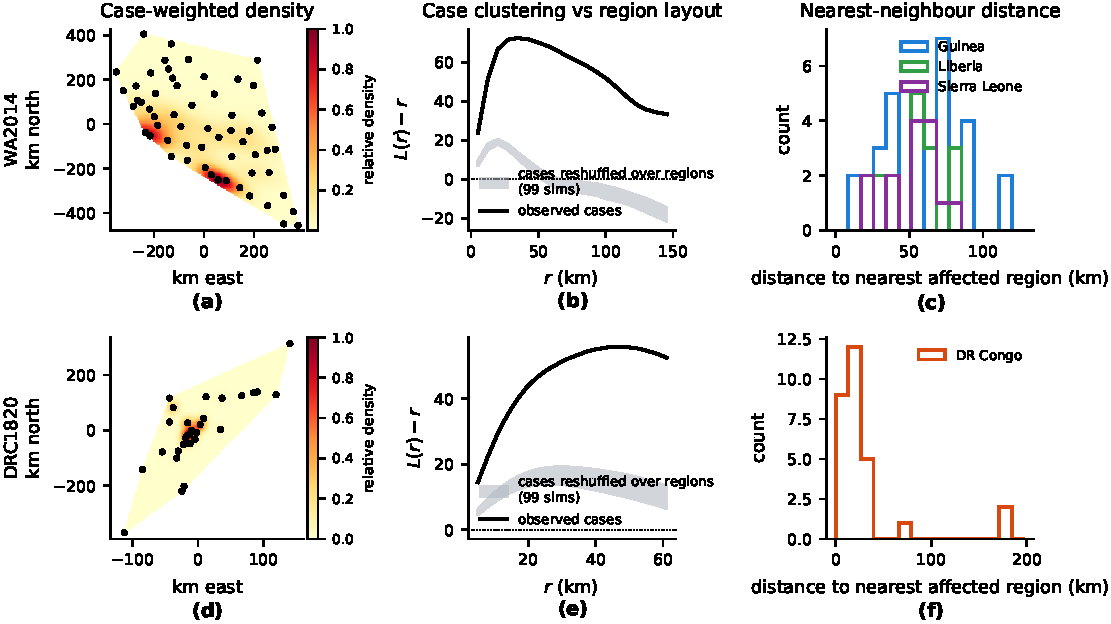
\includegraphics[width=\textwidth]{figs/pointpattern.pdf}
\caption{Spatial point-pattern decomposition of the two outbreaks, WA2014 in (a)--(c) and DRC1820 in (d)--(f): (a,d)~case-weighted kernel density, (b,e)~Ripley's $L(r)-r$ for the case point pattern against a 99-simulation envelope in which the same cases are reshuffled over the same region seats, (c,f)~distance from each affected region to its nearest affected neighbour.}
\label{fig:pointpattern}
\end{figure*}

\begin{figure*}[t]
\centering
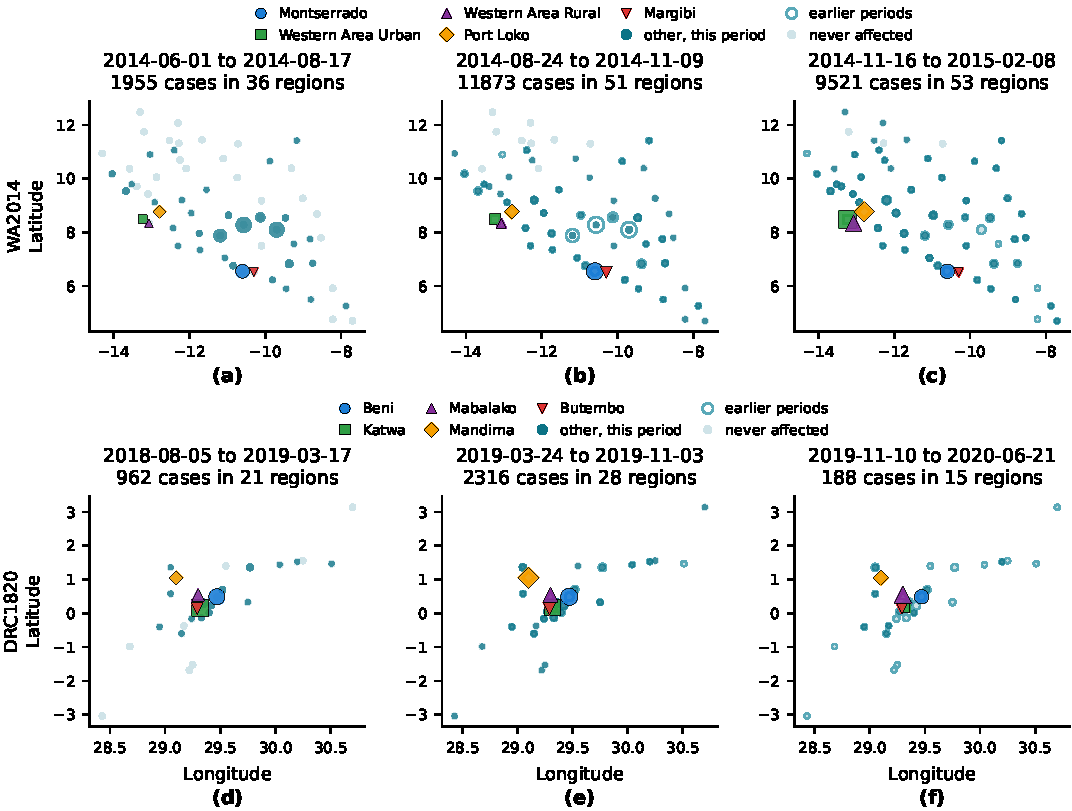
\includegraphics[width=\textwidth]{figs/spread.pdf}
\caption{Spatio-temporal spread of both modelled panels in three equal periods: WA2014 in (a)--(c) and DRC1820 in (d)--(f), each running from the earliest period on the left to the latest on the right. Coloured markers are each outbreak's five largest cumulative hot spots, held to the same symbol across periods; solid teal marks other regions active in the current period, open teal rings those active only earlier, and pale teal those never affected.}
\label{fig:spread}
\end{figure*}

\begin{figure*}[t]
\centering
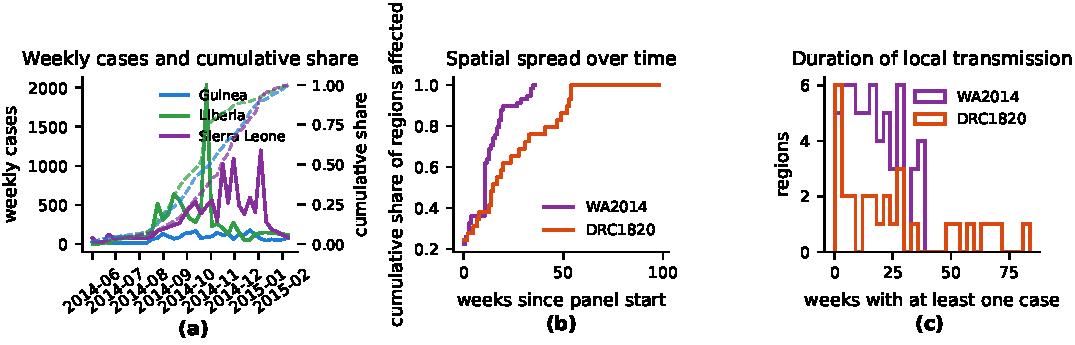
\includegraphics[width=\textwidth]{figs/temporal.pdf}
\caption{Temporal decomposition: (a)~weekly cases and cumulative share by West African country, (b)~cumulative share of regions ever affected, (c)~number of weeks each region reported at least one case.}
\label{fig:temporal}
\end{figure*}

\subsection{Spatial and temporal structure of the panels}\label{sec:structure}

Before modelling we characterise what the two outbreaks look like as point patterns, because the structure explains which model components matter later.

\textbf{Cases cluster far beyond the region layout.} Administrative seats are close to regularly spaced by construction, so testing regions against complete spatial randomness is uninformative. Fig.~\ref{fig:pointpattern}(b) therefore holds the layout fixed and reshuffles the observed cases over the same seats. The observed $L(r)-r$ lies above that envelope at \emph{every} distance tested on both panels, peaking at $72$ (WA2014, $r\approx\SI{35}{km}$) and $56$ (DRC1820, $r\approx\SI{45}{km}$). Transmission is thus concentrated in a few adjacent regions rather than spread across the affected area, which is what makes a spatial operator worth learning at all.

\textbf{The two panels differ in scale, not in kind.} The affected window covers \SI{337000}{km^2} and 58 regions in WA2014 against \SI{59600}{km^2} and 29 health zones in DRC1820, and the median distance to the nearest affected neighbour is \SI{58}{km} against \SI{20}{km} (Fig.~\ref{fig:pointpattern}(c)). The Guinean distribution has the long right tail, consistent with the dispersed prefecture-level introductions that the genomic prior later picks up.


\begin{figure*}[t]
\centering
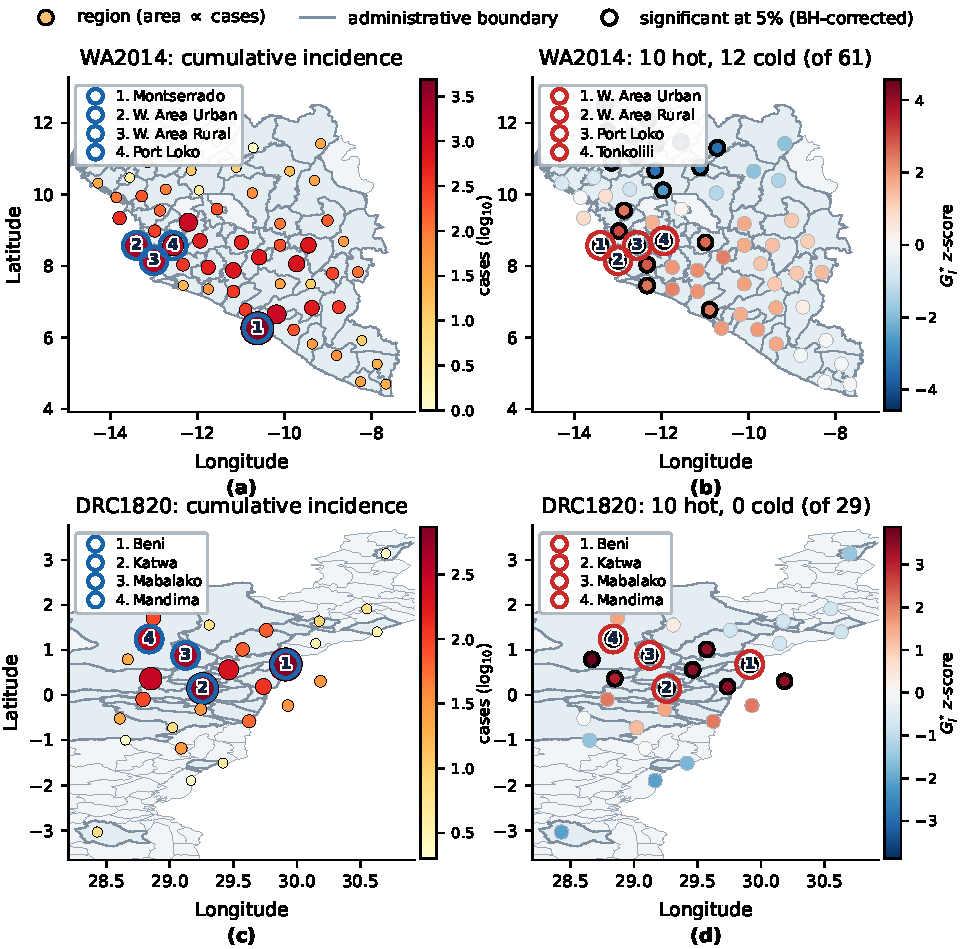
\includegraphics[width=\textwidth]{figs/hotspot.pdf}
\caption{Where the cases are, and where that concentration is statistically unusual. WA2014 in (a,b) and DRC1820 in (c,d). (a,c)~cumulative incidence per region, by colour and marker area, over the administrative boundaries of the modelled units. (b,d)~the Getis-Ord $G_i^{\star}$ $z$-score of $\log(1{+}\text{cases})$ on the same axes (8 nearest neighbours), with a black ring on regions significant at 5\% after Benjamini--Hochberg correction. The four largest regions and the four largest hot spots are numbered and named in the corner keys. Marker positions are relaxed by a small repulsion where seats nearly coincide, so the dense North Kivu cluster is legible; the statistic itself is computed on the recorded coordinates.}
\label{fig:hotspot}
\end{figure*}

\textbf{Concentration is statistically unusual, and differently so on the two panels.} Fig.~\ref{fig:hotspot} places cumulative incidence and a Getis-Ord $G_i^{\star}$ test on common axes, so the statistic can be read against the case distribution that produced it. We test $\log(1{+}\text{cases})$ rather than raw counts, because the raw distribution is dominated by a handful of districts and no region reaches significance under it; this is the usual transform for skewed count data and we state it rather than selecting the version that gives more stars. On WA2014 the test finds 10 hot spots and 12 cold spots among 61 districts: the hot cluster runs along the Guinea--Sierra Leone border and through the Western Area, and the cold one covers the northern Guinean prefectures that were never seriously affected. On DRC1820 it finds 10 hot zones and \emph{no} cold ones among 29, because every zone in the panel is part of one outbreak; those 10 carry 87\% of all cases, against 37\% for the West African hot spots. This is the same contrast as the point-pattern analysis: one spatially concentrated epidemic in North Kivu, and one multi-country epidemic with a broad affected area and a few intense corridors.

\textbf{Spread and persistence.} Fig.~\ref{fig:spread} shows the outbreaks reaching 36, 51 and 53 regions in successive thirds of WA2014, and 21, 28 then 15 in DRC1820, where the third period is the tail. Holding each outbreak's five largest hot spots to a fixed symbol makes the internal shift visible: West Africa's weight stays on Montserrado and the Western Area throughout, whereas in DR~Congo it moves from Mabalako and Beni in the first period to Mandima and Katwa in the second. Fig.~\ref{fig:temporal}(b) shows West Africa saturating its regions within about 20 weeks while DR~Congo takes roughly 50, and Fig.~\ref{fig:temporal}(c) that most regions sustain transmission for fewer than 30 weeks with a small number persisting far longer. These are the long, low-count chains that the renewal decoder tracks well and the baselines over-smooth (RQ5).


\begin{figure*}[t]
\centering
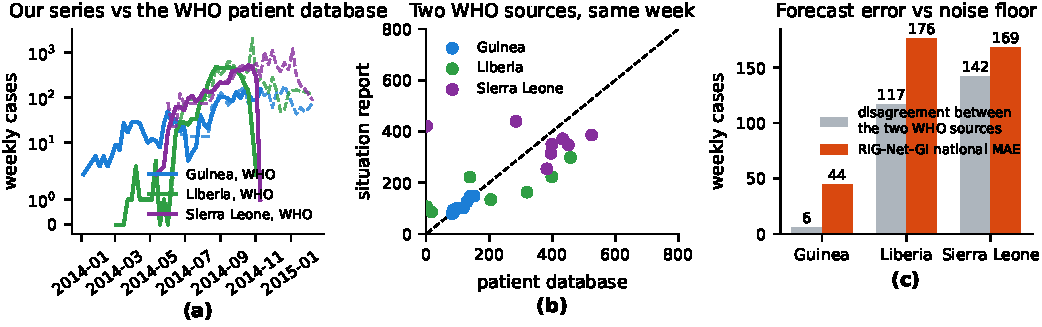
\includegraphics[width=\textwidth]{figs/sources.pdf}
\caption{External check against the WHO 2014-11-12 data package, which counts the same country-week twice. (a)~our cleaned national series against the WHO patient database; (b)~the two WHO sources against each other on the weeks both report; (c)~our national forecast error beside the disagreement between those two sources.}
\label{fig:sources}
\end{figure*}

\subsection{External validation and the observation-error floor}\label{sec:sources}

Our WA2014 panel is built from one compilation of situation reports, so it inherits whatever errors that compilation contains. The WHO 2014-11-12 data package provides an independent check, because it reports each country-week twice: once from situation reports and once from a reconstructed patient database. We use it two ways.

\textbf{Does our cleaning reproduce an independent reconstruction?} For Guinea and Sierra Leone, yes: our weekly national series correlates $0.93$ and $0.82$ with the WHO patient database over 24 overlapping weeks, with cumulative totals within 1\% and 7\% (Fig.~\ref{fig:sources}(a)). For Liberia it does not: the correlation is $0.20$ and our total exceeds WHO's by 62\% (6{,}938 against 4{,}277). This is an independent confirmation of the artefact we already flagged, the Montserrado backlog, which the ROWCA compilation books in the week it was reconciled and the patient database redistributes to the weeks of onset. Liberia is therefore the one country whose panel should be treated as unreliable at weekly resolution, and it is also where our model performs worst at national level (RQ5).

\textbf{How much can any forecaster be expected to achieve?} Fig.~\ref{fig:sources}(b) compares the two WHO sources on the seven to eight weeks both cover. They disagree by a mean of 5.9 cases per week for Guinea (5.4\% in relative terms), 117 for Liberia (83\%) and 142 for Sierra Leone (49\%). This is a measured floor on observation error: two official sources, describing the same weeks of the same epidemic, differ by this much. Fig.~\ref{fig:sources}(c) places our national forecast error beside it. For Sierra Leone the model's MAE is $1.19\times$ the inter-source disagreement and for Liberia $1.50\times$; only for Guinea, where the sources nearly agree, is the ratio large ($7.6\times$).

We draw a deliberately restrained conclusion. For two of the three West African countries, a one-week-ahead forecast is already within roughly 20--50\% of the disagreement between two official records of what actually happened, so further MAE reductions on those panels are competing with the resolution of the ground truth rather than with the epidemiology. This does not excuse the model's errors, but it does bound how much of the remaining gap is recoverable, and it is a reason to prefer calibrated intervals (RQ9) over point accuracy as the operational target.

\subsection{Metrics}\label{sec:metrics}

Let $y_i(t)$ be the observed count in region $i$ at week $t$, $\hat y_i(t)$ the point forecast, and $\mathcal{T}$ the set of scored region--week--horizon triples with $|\mathcal{T}|=n$. The two primary metrics are
\begin{equation}
\begin{aligned}
\mathrm{MAE}&=\frac1n\!\!\sum_{(i,t)\in\mathcal{T}}\!\!\big|\hat y_i(t)-y_i(t)\big|,\\[2pt]
\mathrm{RMSE}&=\Big(\frac1n\!\!\sum_{(i,t)\in\mathcal{T}}\!\!\big(\hat y_i(t)-y_i(t)\big)^2\Big)^{1/2}.
\end{aligned}
\label{eq:mae}
\end{equation}
MAE is reported first because the predictive median is its Bayes act~\cite{gneiting2011}; RMSE is retained because it is more sensitive to the large errors that occur at epidemic peaks. Linear agreement is measured by the Pearson correlation
\begin{equation}
\mathrm{PCC}=\frac{\sum_{(i,t)}(\hat y_i(t)-\bar{\hat y})(y_i(t)-\bar y)}
{\sqrt{\sum_{(i,t)}(\hat y_i(t)-\bar{\hat y})^2}\sqrt{\sum_{(i,t)}(y_i(t)-\bar y)^2}}.
\label{eq:pcc}
\end{equation}
Because absolute errors are not comparable across panels of very different size, we also report two scale-free metrics. MASE divides by the in-sample one-step naive error~\cite{hyndman2006}, and sMAPE is bounded and symmetric in over- and under-prediction:
\begin{equation}
\mathrm{MASE}=\frac{\frac1n\sum_{(i,t)}|\hat y_i(t)-y_i(t)|}
{\frac{1}{T-1}\sum_{t=2}^{T}|y_i(t)-y_i(t-1)|},
\label{eq:mase}
\end{equation}
\begin{equation}
\mathrm{sMAPE}=\frac{100}{n}\!\!\sum_{(i,t)\in\mathcal{T}}\!\!
\frac{|\hat y_i(t)-y_i(t)|}{\big(|y_i(t)|+|\hat y_i(t)|\big)/2}.
\label{eq:smape}
\end{equation}
For the probabilistic head we report the empirical coverage of the central $1-\alpha$ interval $[q_{\alpha/2},q_{1-\alpha/2}]$ and the weighted interval score~\cite{bracher2021}, with $\mathbf{1}\{\cdot\}$ the indicator:
\begin{equation}
\mathrm{Cov}_{1-\alpha}=\frac1n\!\!\sum_{(i,t)\in\mathcal{T}}\!\!
\mathbf{1}\big\{q_{\alpha/2}\leq y_i(t)\leq q_{1-\alpha/2}\big\}.
\label{eq:cov}
\end{equation}
Finally, peak-week error is the absolute difference between the week of the predicted and the observed local maximum, over regions with more than 20 cases, and all metrics are computed per seed and reported as mean $\pm$ standard deviation over the five seeds.

\subsection{Protocol}

A single chronological split proved uninformative: placing the DRC test period in February--June 2020, when 0.1 cases per zone-week were reported, made the naive forecast unbeatable. We therefore use \emph{rolling-origin} evaluation with seven non-overlapping test blocks spanning the epidemic curve: WA2014 peak (12 Oct--16 Nov 2014), decline (23 Nov--28 Dec 2014) and tail (4 Jan--8 Feb 2015); DRC1820 growth (14 Apr--30 Jun 2019), plateau (7 Jul--22 Sep 2019), decline (29 Sep--15 Dec 2019) and tail (22 Dec 2019--8 Mar 2020). For a block starting at week $s$, validation is the preceding $\max(4,0.2s)$ weeks and training is everything earlier; the scaler, the genomic cut-off and the standardisation of $\mathbf{u}$ are all fitted on that fold's training weeks only.

All models use Adam, full-batch training, at most 300 epochs and early stopping on validation MAE (patience 40). Each baseline selects its learning rate from $\{10^{-3},3\times10^{-3}\}$ per fold and seed on validation MAE. RIG-Net uses $d=64$, lr $3\times10^{-3}$ ($\approx$41k parameters, within the 56--55{,}000 range of the baselines), $R_{\max}=2.5$, $\kappa=3$, $\lambda=0.1$, fixed by a validation-only search before any test result was inspected. Five random seeds are run for every model, giving 1{,}446 training runs. We report MAE, RMSE and Pearson correlation in weekly cases per region, pooled over all scored region--horizon--week points, as mean $\pm$ standard deviation over the five seeds. Significance uses the Diebold--Mariano (DM) test on paired absolute-error differentials of seed-averaged forecasts.

\subsection{Baselines}

Sixteen models published 2020--2026 are re-implemented in PyTorch: eight temporal forecasters (N-BEATS~\cite{nbeats}, Autoformer~\cite{autoformer}, DLinear~\cite{dlinear}, N-HiTS~\cite{nhits}, PatchTST~\cite{patchtst}, TimesNet~\cite{timesnet}, TSMixer~\cite{tsmixer}, iTransformer~\cite{itransformer}) and eight spatio-temporal graph models (AGCRN~\cite{agcrn}, MTGNN~\cite{mtgnn}, Cola-GNN~\cite{colagnn}, EpiGNN~\cite{epignn}, STID~\cite{stid}, MepoGNN~\cite{mepognn}, STAEformer~\cite{staeformer}, MAST-Net~\cite{mastnet}), plus two non-learned references (last-value and 3-week mean). These are compact re-implementations of each paper's core mechanism sized for panels of at most 61 regions, not the authors' official code. MAST-Net~\cite{mastnet} is the most recent of these and was published after the rest of this benchmark was assembled; its full text was not accessible to us, so our version follows the three mechanisms its abstract and section headings describe, manifold-preserving learnable augmentation, parallel multi-scale graph convolution, and a Lipschitz-constrained temporal module, and should be read as a reconstruction from that description rather than a reproduction.

\section{Results}\label{sec:results}

We organise the evaluation around fourteen research questions.
\textbf{RQ1} How accurate is RIG-Net-GI against 15 recent baselines?
\textbf{RQ2} What does each component contribute?
\textbf{RQ3} How does performance depend on epidemic phase and forecast horizon?
\textbf{RQ4} Does validation performance transfer to the test blocks?
\textbf{RQ5} Where and when, in space and time, does the model win or lose?
\textbf{RQ6} Are the learned epidemiological quantities meaningful?
\textbf{RQ7} Do the theoretical results hold empirically?
\textbf{RQ8} What does the genomic prior actually encode?
\textbf{RQ9} Is the forecast distribution calibrated, and how does the model score on scale-free metrics?
\textbf{RQ10} How does health-system access and genomic surveillance differ across the four countries, and does it matter for the model?
\textbf{RQ11} How do the models behave during training?
\textbf{RQ12} Is the protocol leak-free, is the learned $R$ a real reproduction number, and is the forecast distribution calibrated?
\textbf{RQ13} How sensitive is the model to its hyper-parameters and graph construction, and what does it cost?
\textbf{RQ14} What onward-transmission network does the model predict in each country?

\begin{table*}[t]
\caption{Pooled test metrics as mean $\pm$ standard deviation over 5 random seeds and 7 rolling-origin blocks. MAE and RMSE in weekly cases per region. The two reference forecasters~\cite{hyndman2006} are deterministic; they were nonetheless run at all five seeds, and their measured standard deviation is zero. Rank is by MAE among the 19 systems compared. Ablations and unpriored variants are in Table~\ref{tab:ablation}. Within each column, \textbf{best}, \underline{second} and \uuline{third} are marked. Our model is listed last.}
\label{tab:main}
\centering\footnotesize
\setlength{\tabcolsep}{3.2pt}
\begin{tabular}{llcccr@{\hskip 8pt}cccr}
\toprule
\multirow{2}{*}{Model} & \multirow{2}{*}{Venue} & \multicolumn{4}{c}{WA2014} & \multicolumn{4}{c}{DRC1820} \\
\cmidrule(lr){3-6}\cmidrule(lr){7-10}
 & & MAE & RMSE & PCC & Rk & MAE & RMSE & PCC & Rk \\
\midrule
MTGNN & KDD'20 & \textbf{11.38\,$\pm$\,0.43} & 60.42\,$\pm$\,0.66 & 0.385\,$\pm$\,0.028 & 1 & \underline{1.300\,$\pm$\,0.021} & \uuline{3.89\,$\pm$\,0.05} & \uuline{0.699\,$\pm$\,0.012} & 2 \\
N-BEATS & ICLR'20 & \underline{11.52\,$\pm$\,0.08} & 60.28\,$\pm$\,0.59 & 0.382\,$\pm$\,0.015 & 2 & 1.307\,$\pm$\,0.006 & 3.90\,$\pm$\,0.03 & 0.679\,$\pm$\,0.006 & 6 \\
Cola-GNN & CIKM'20 & \uuline{11.81\,$\pm$\,0.31} & \uuline{59.94\,$\pm$\,0.44} & 0.400\,$\pm$\,0.016 & 3 & 1.307\,$\pm$\,0.013 & \textbf{3.80\,$\pm$\,0.02} & \underline{0.706\,$\pm$\,0.002} & 5 \\
STID & CIKM'22 & 12.40\,$\pm$\,0.35 & 61.29\,$\pm$\,0.82 & 0.387\,$\pm$\,0.014 & 7 & 1.302\,$\pm$\,0.010 & \underline{3.88\,$\pm$\,0.02} & 0.689\,$\pm$\,0.004 & 4 \\
EpiGNN & ECML'22 & 12.42\,$\pm$\,0.43 & \underline{59.68\,$\pm$\,1.24} & \uuline{0.403\,$\pm$\,0.039} & 8 & \uuline{1.302\,$\pm$\,0.020} & 3.94\,$\pm$\,0.12 & 0.676\,$\pm$\,0.020 & 3 \\
N-HiTS & AAAI'23 & 12.27\,$\pm$\,0.31 & 62.82\,$\pm$\,0.56 & 0.325\,$\pm$\,0.008 & 6 & 1.310\,$\pm$\,0.012 & 3.92\,$\pm$\,0.03 & 0.674\,$\pm$\,0.007 & 7 \\
iTransformer & ICLR'24 & 12.44\,$\pm$\,0.29 & 65.09\,$\pm$\,1.76 & 0.338\,$\pm$\,0.013 & 9 & 1.323\,$\pm$\,0.012 & 3.98\,$\pm$\,0.03 & 0.669\,$\pm$\,0.006 & 8 \\
MAST-Net & JNCA'26 & 12.14\,$\pm$\,0.23 & 61.12\,$\pm$\,0.22 & 0.345\,$\pm$\,0.007 & 5 & 1.464\,$\pm$\,0.030 & 4.51\,$\pm$\,0.05 & 0.612\,$\pm$\,0.016 & 13 \\
DLinear & AAAI'23 & 12.64\,$\pm$\,0.57 & 62.20\,$\pm$\,1.83 & \underline{0.407\,$\pm$\,0.014} & 10 & 1.326\,$\pm$\,0.014 & 3.99\,$\pm$\,0.03 & 0.673\,$\pm$\,0.007 & 9 \\
STAEformer & CIKM'23 & 12.69\,$\pm$\,0.51 & 61.26\,$\pm$\,0.10 & 0.337\,$\pm$\,0.007 & 11 & 1.351\,$\pm$\,0.036 & 4.10\,$\pm$\,0.10 & 0.666\,$\pm$\,0.024 & 11 \\
PatchTST & ICLR'23 & 13.01\,$\pm$\,0.15 & 67.36\,$\pm$\,1.17 & 0.327\,$\pm$\,0.009 & 12 & 1.326\,$\pm$\,0.008 & 3.98\,$\pm$\,0.01 & 0.667\,$\pm$\,0.002 & 10 \\
TimesNet & ICLR'23 & 13.40\,$\pm$\,0.43 & 61.79\,$\pm$\,1.18 & 0.321\,$\pm$\,0.056 & 13 & 1.770\,$\pm$\,0.019 & 4.89\,$\pm$\,0.08 & 0.408\,$\pm$\,0.036 & 16 \\
Naive (ref.) & \cite{hyndman2006} & 14.48\,$\pm$\,0.00 & 79.64\,$\pm$\,0.00 & 0.261\,$\pm$\,0.000 & 17 & 1.407\,$\pm$\,0.000 & 4.08\,$\pm$\,0.00 & \textbf{0.708\,$\pm$\,0.000} & 12 \\
MA3 (ref.) & \cite{hyndman2006} & 14.37\,$\pm$\,0.00 & 66.46\,$\pm$\,0.00 & 0.343\,$\pm$\,0.000 & 16 & 1.474\,$\pm$\,0.000 & 4.18\,$\pm$\,0.00 & 0.673\,$\pm$\,0.000 & 14 \\
Autoformer & NeurIPS'21 & 13.45\,$\pm$\,0.41 & 64.34\,$\pm$\,0.82 & 0.211\,$\pm$\,0.057 & 14 & 1.802\,$\pm$\,0.073 & 5.37\,$\pm$\,0.32 & 0.273\,$\pm$\,0.089 & 18 \\
AGCRN & NeurIPS'20 & 15.26\,$\pm$\,0.39 & 61.57\,$\pm$\,0.97 & 0.331\,$\pm$\,0.033 & 18 & 1.619\,$\pm$\,0.050 & 4.72\,$\pm$\,0.09 & 0.469\,$\pm$\,0.033 & 15 \\
MepoGNN & ECML'22 & 14.20\,$\pm$\,0.34 & 62.27\,$\pm$\,0.53 & 0.291\,$\pm$\,0.027 & 15 & 1.822\,$\pm$\,0.082 & 5.83\,$\pm$\,0.54 & 0.483\,$\pm$\,0.023 & 19 \\
TSMixer & TMLR'23 & 15.64\,$\pm$\,1.51 & 72.67\,$\pm$\,5.91 & 0.139\,$\pm$\,0.082 & 19 & 1.801\,$\pm$\,0.042 & 5.30\,$\pm$\,0.20 & 0.285\,$\pm$\,0.105 & 17 \\
\midrule
\textbf{RIG-Net-GI (ours)} & --- & 11.91\,$\pm$\,0.46 & \textbf{58.22\,$\pm$\,0.88} & \textbf{0.453\,$\pm$\,0.030} & 4 & \textbf{1.247\,$\pm$\,0.020} & 4.15\,$\pm$\,0.05 & 0.689\,$\pm$\,0.007 & 1 \\
\bottomrule
\end{tabular}
\end{table*}

\subsection{RQ1: accuracy against 16 baselines}

Table~\ref{tab:main} gives pooled results. On DRC1820 RIG-Net-GI attains the lowest MAE of all 19 systems ($1.247\pm0.020$ against $1.300\pm0.021$ for the best baseline, MTGNN), and the Diebold--Mariano test rejects equality in its favour against \emph{all sixteen} baselines (Table~\ref{tab:dm}, every DRC1820 row marked $\blacktriangle$) at $p<0.05$. On WA2014 it ranks fourth by MAE ($11.91\pm0.46$ against $11.38\pm0.43$) while attaining the best RMSE ($58.22$ against $59.94$) and the best correlation ($0.453$ against $0.407$) of any system; the DM test (Table~\ref{tab:dm}) places it significantly ahead of 7 baselines, tied with 8 (N-BEATS, Cola-GNN, EpiGNN, STID, N-HiTS, DLinear, iTransformer, MAST-Net) and significantly behind only MTGNN ($p=0.001$).

That RIG-Net-GI leads on RMSE and correlation while trailing slightly on MAE in WA2014 is informative: the renewal decoder tracks the shape of the epidemic curve better, so large errors are rarer, but it pays a small penalty on the many near-zero region-weeks that dominate MAE. RQ5 localises exactly where this happens.

Two patterns are visible among the baselines. Simple, strongly regularised models (MTGNN, N-BEATS, N-HiTS) are the hardest to beat, while heavier architectures designed for long periodic series (TimesNet, Autoformer, TSMixer) and the SIR hybrid MepoGNN fall below the naive reference on at least one panel. Graph structure per se confers no consistent advantage: the best temporal and best graph baselines differ by under 1\% on DRC1820.


\begin{table*}[t]
\centering
\caption{Comprehensive ablation of RIG-Net-GI, mean $\pm$ standard deviation over 5 random seeds and all rolling-origin blocks. \cmark\ indicates the component is included, \xmark\ that it is removed. Components: \textbf{REN} renewal decoder; \textbf{STB} stabilisation ($R_{\max}{=}2.5$, pressure clip $\kappa{=}3$); \textbf{GEO}/\textbf{ADP}/\textbf{DYN} geographic, learned-static and attention adjacencies; \textbf{GEN} genomic transmission-linkage prior; \textbf{KL} genomic consistency regulariser; \textbf{INT} intervention-aware suppression; \textbf{NB} negative-binomial likelihood. The upper block ablates the full model; the lower block ablates the unpriored model, the base those components were introduced on. MAE and RMSE in weekly cases per region.}
\label{tab:ablation}
\resizebox{\linewidth}{!}{%
\fontsize{7}{8.5}\selectfont
\setlength{\tabcolsep}{3pt}
\renewcommand{\arraystretch}{0.95}
\begin{tabular}{lcccccccc cccc}
\hline
\multirow{2}{*}{\textbf{Model variant}} & \multicolumn{8}{c}{\textbf{Components}} & \multicolumn{2}{c}{\textbf{WA2014}} & \multicolumn{2}{c}{\textbf{DRC1820}} \\
\cline{2-9}\cline{10-11}\cline{12-13}
 & \textbf{REN} & \textbf{STB} & \textbf{GEO} & \textbf{ADP} & \textbf{DYN} & \textbf{GEN} & \textbf{KL} & \textbf{INT} & \textbf{MAE} & \textbf{RMSE} & \textbf{MAE} & \textbf{RMSE} \\
 & ($w$) & ($R_{\max},\kappa$) & ($A^{\mathrm{geo}}$) & ($A^{\mathrm{adp}}$) & ($A^{\mathrm{dyn}}$) & ($A^{\mathrm{gen}}$) & ($\lambda$) & ($\boldsymbol{\beta}$) & & & & \\
\hline
\textbf{RIG-Net-GI (full)} & \cmark & \cmark & \cmark & \cmark & \cmark & \cmark & \cmark & \cmark & 11.91\,$\pm$\,0.46 & 58.22\,$\pm$\,0.88 & 1.247\,$\pm$\,0.020 & 4.15\,$\pm$\,0.05 \\
\hline
w/o KL regulariser & \cmark & \cmark & \cmark & \cmark & \cmark & \cmark & \xmark & \cmark & 11.98\,$\pm$\,0.58 & 58.33\,$\pm$\,0.90 & 1.243\,$\pm$\,0.020 & 4.13\,$\pm$\,0.05 \\
w/o intervention term & \cmark & \cmark & \cmark & \cmark & \cmark & \cmark & \cmark & \xmark & 12.32\,$\pm$\,0.64 & 58.04\,$\pm$\,0.42 & 1.224\,$\pm$\,0.026 & 4.03\,$\pm$\,0.08 \\
w/o genomic prior & \cmark & \cmark & \cmark & \cmark & \cmark & \xmark & \xmark & \cmark & 12.21\,$\pm$\,0.54 & 58.32\,$\pm$\,0.84 & 1.238\,$\pm$\,0.028 & 4.10\,$\pm$\,0.07 \\
w/o both priors (RIG-Net-S) & \cmark & \cmark & \cmark & \cmark & \cmark & \xmark & \xmark & \xmark & 13.24\,$\pm$\,1.17 & 58.19\,$\pm$\,0.90 & 1.231\,$\pm$\,0.024 & 4.04\,$\pm$\,0.03 \\
\hline
\multicolumn{13}{l}{\emph{Unpriored base (components introduced before the priors; $R_{\max}{=}4$, no clip)}}\\
\hline
RIG-Net (unpriored base) & \cmark & \xmark & \cmark & \cmark & \cmark & \xmark & \xmark & \xmark & 15.07\,$\pm$\,2.95 & 62.57\,$\pm$\,3.34 & 1.295\,$\pm$\,0.047 & 4.14\,$\pm$\,0.02 \\
\quad w/o renewal decoder & \xmark & \xmark & \cmark & \cmark & \cmark & \xmark & \xmark & \xmark & 14.10\,$\pm$\,0.91 & 61.75\,$\pm$\,1.55 & 1.254\,$\pm$\,0.015 & 3.97\,$\pm$\,0.06 \\
\quad w/o geographic graph & \cmark & \xmark & \xmark & \cmark & \cmark & \xmark & \xmark & \xmark & 14.48\,$\pm$\,1.21 & 62.02\,$\pm$\,0.77 & 1.246\,$\pm$\,0.015 & 4.06\,$\pm$\,0.08 \\
\quad w/o learned-static graph & \cmark & \xmark & \cmark & \xmark & \cmark & \xmark & \xmark & \xmark & 14.74\,$\pm$\,1.74 & 62.29\,$\pm$\,1.18 & 1.265\,$\pm$\,0.023 & 4.13\,$\pm$\,0.06 \\
\quad w/o attention graph & \cmark & \xmark & \cmark & \cmark & \xmark & \xmark & \xmark & \xmark & 12.81\,$\pm$\,0.75 & 60.38\,$\pm$\,0.67 & 1.267\,$\pm$\,0.026 & 4.12\,$\pm$\,0.02 \\
\quad w/o NB likelihood & \cmark & \xmark & \cmark & \cmark & \cmark & \xmark & \xmark & \xmark & 13.07\,$\pm$\,0.91 & 61.22\,$\pm$\,0.97 & 1.324\,$\pm$\,0.030 & 4.11\,$\pm$\,0.08 \\
\hline
\end{tabular}%
}
\end{table*}

\begin{table}[t]
\centering
\caption{Pairwise Diebold--Mariano tests of RIG-Net-GI against every baseline, on region--week--horizon loss differentials. $\Delta$MAE is the baseline's MAE minus ours, so positive favours our model. $p_{\mathrm{Holm}}$ is Holm-corrected within each dataset over the 18 comparisons. $\blacktriangle$ we are significantly better, $\blacktriangledown$ significantly worse, $\approx$ no significant difference at 5\%.}
\label{tab:dm}
\resizebox{\columnwidth}{!}{%
\begin{tabular}{lrrrcrrrc}
\toprule
 & \multicolumn{4}{c}{WA2014} & \multicolumn{4}{c}{DRC1820} \\
\cmidrule(lr){2-5}\cmidrule(lr){6-9}
Baseline & $\Delta$MAE & DM & $p_{\mathrm{Holm}}$ & & $\Delta$MAE & DM & $p_{\mathrm{Holm}}$ & \\
\midrule
MTGNN & -0.52 & -3.40 & 0.007 & $\blacktriangledown$ & +0.053 & 3.08 & 0.004 & $\blacktriangle$ \\
N-BEATS & -0.39 & -1.20 & 0.924 & $\approx$ & +0.060 & 3.63 & 0.002 & $\blacktriangle$ \\
Cola-GNN & -0.09 & 0.23 & 0.924 & $\approx$ & +0.060 & 3.68 & 0.002 & $\blacktriangle$ \\
STID & +0.49 & 1.77 & 0.538 & $\approx$ & +0.055 & 3.32 & 0.004 & $\blacktriangle$ \\
EpiGNN & +0.52 & 1.16 & 0.924 & $\approx$ & +0.055 & 3.02 & 0.004 & $\blacktriangle$ \\
N-HiTS & +0.36 & 1.65 & 0.597 & $\approx$ & +0.063 & 3.51 & 0.003 & $\blacktriangle$ \\
iTransformer & +0.53 & 1.14 & 0.924 & $\approx$ & +0.077 & 3.20 & 0.004 & $\blacktriangle$ \\
MAST-Net & +0.24 & 1.89 & 0.475 & $\approx$ & +0.217 & 17.19 & 0.000 & $\blacktriangle$ \\
DLinear & +0.73 & 1.46 & 0.720 & $\approx$ & +0.079 & 6.01 & 0.000 & $\blacktriangle$ \\
STAEformer & +0.79 & 4.37 & 0.000 & $\blacktriangle$ & +0.104 & 7.68 & 0.000 & $\blacktriangle$ \\
PatchTST & +1.10 & 2.41 & 0.142 & $\approx$ & +0.079 & 3.48 & 0.003 & $\blacktriangle$ \\
TimesNet & +1.49 & 5.49 & 0.000 & $\blacktriangle$ & +0.523 & 24.78 & 0.000 & $\blacktriangle$ \\
Autoformer & +1.55 & 4.50 & 0.000 & $\blacktriangle$ & +0.555 & 20.48 & 0.000 & $\blacktriangle$ \\
AGCRN & +3.35 & 11.56 & 0.000 & $\blacktriangle$ & +0.372 & 17.75 & 0.000 & $\blacktriangle$ \\
MepoGNN & +2.30 & 10.50 & 0.000 & $\blacktriangle$ & +0.575 & 9.70 & 0.000 & $\blacktriangle$ \\
TSMixer & +3.73 & 5.22 & 0.000 & $\blacktriangle$ & +0.554 & 22.30 & 0.000 & $\blacktriangle$ \\
Naive & +2.57 & 3.62 & 0.003 & $\blacktriangle$ & +0.160 & 4.55 & 0.000 & $\blacktriangle$ \\
MA3 & +2.47 & 5.96 & 0.000 & $\blacktriangle$ & +0.227 & 6.56 & 0.000 & $\blacktriangle$ \\
\bottomrule
\end{tabular}}
\end{table}

\subsection{RQ2: component contributions}

Table~\ref{tab:ablation} isolates each component. Starting from the unpriored, unstabilised model ($15.07\pm2.96$ on WA2014, $1.295\pm0.047$ on DRC1820), bounding $R_{\max}$ and clipping the renewal pressure removes the peak blow-up and cuts the seed variance by a factor of about 2.5 ($13.24\pm1.17$, $1.231\pm0.024$). Adding the genomic prior is the single largest further gain on WA2014: removing it from the full model costs $+0.31$ MAE ($11.91\rightarrow12.21$), consistent with its gate weight of 28\% there. The genomic KL term is within seed noise on both panels ($\mp0.08$ and $\mp0.004$).

The intervention term behaves asymmetrically. On WA2014 it helps ($12.32\rightarrow11.91$ when added), whereas on DRC1820 the variant \emph{without} it is the best configuration overall ($1.224\pm0.026$ against $1.247\pm0.020$, a gap within one seed standard deviation). We report this plainly: on DRC1820 the full model is not the best variant, and the gain there comes from stabilisation and the genomic channel rather than from intervention modulation.

\subsection{RQ3: epidemic phase and forecast horizon}

\begin{figure}[t]
\centering
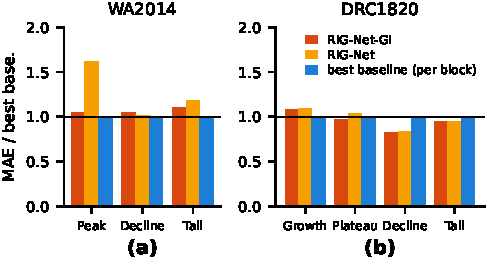
\includegraphics[width=\columnwidth]{figs/phase.pdf}
\caption{MAE relative to the best baseline in each test block (1.0 = best baseline, lower is better), for (a)~WA2014 and (b)~DRC1820. The priored model is strongest in decline and tail phases and weakest at the explosive WA peak, as Theorem~\ref{thm:error} predicts.}
\label{fig:phase}
\end{figure}

\begin{figure}[t]
\centering
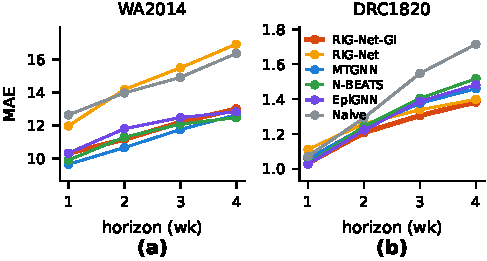
\includegraphics[width=\columnwidth]{figs/horizon.pdf}
\caption{MAE by forecast horizon, for (a)~WA2014 and (b)~DRC1820. The advantage on DRC1820 widens with lead time, consistent with the bounded error accumulation of Theorem~\ref{thm:error} when $\bar R<1$.}
\label{fig:horizon}
\end{figure}

Fig.~\ref{fig:phase} shows error relative to the best baseline per block. RIG-Net-GI leads in the DRC decline (0.495 against 0.673 for MTGNN, $-26\%$) and the DRC tail (0.287 against 0.389, $-26\%$), and trails at the WA peak (16.09 against 15.34), in the WA decline (10.06 against 9.80) and tail (8.83 against 8.37), and in the DRC growth phase (2.49 against 2.33). Fig.~\ref{fig:horizon} shows the horizon profile: on DRC1820 the model is best at every horizon, and its margin widens with lead time from $1.034$ at one week (best baseline $1.030$) to $1.383$ at four weeks (best baseline $1.460$, a $5\%$ gain). On WA2014 it trails MTGNN at every horizon ($13.01$ against $12.64$ at four weeks), though the gap narrows as the horizon lengthens.

Both patterns follow Theorem~\ref{thm:error}: when $\bar R<1$ the rollout contracts and accumulated parameter error stays bounded, so the renewal decoder should gain at long horizons; when $\bar R>1$ error grows geometrically, so it should lose. The empirical phase and horizon profiles match the predicted signs in all seven blocks.

\subsection{RQ4: does validation performance transfer?}

\begin{figure}[t]
\centering
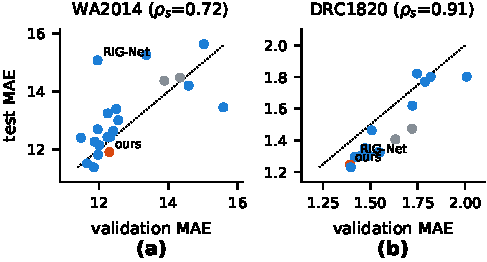
\includegraphics[width=\columnwidth]{figs/val_vs_test.pdf}
\caption{Validation vs test MAE for every model (dotted line is equality), for (a)~WA2014 and (b)~DRC1820. Transfer is strong on DRC1820 (Spearman $\rho_s=0.91$) and weaker on WA2014 ($\rho_s=0.72$), where the unpriored RIG-Net is the clearest outlier: best on validation, worst on test.}
\label{fig:valtest}
\end{figure}

Model selection is only meaningful if validation ranks predict test ranks. Fig.~\ref{fig:valtest} shows they do on DRC1820 (Spearman $\rho_s=0.91$, Pearson $0.92$) but much less on WA2014 ($\rho_s=0.72$, Pearson $0.67$). Each validation block precedes its test block and typically lies in a different epidemic phase, so validation rewards models that extrapolate the current regime. The unpriored RIG-Net is the extreme case: lowest validation MAE of all models on both panels, yet 18th of 19 on WA2014 test. This is why we fixed the variant by a pre-registered validation rule and then reported the result unchanged rather than re-selecting; it is also a caution for single-split studies on a single outbreak.


\begin{figure*}[t]
\centering
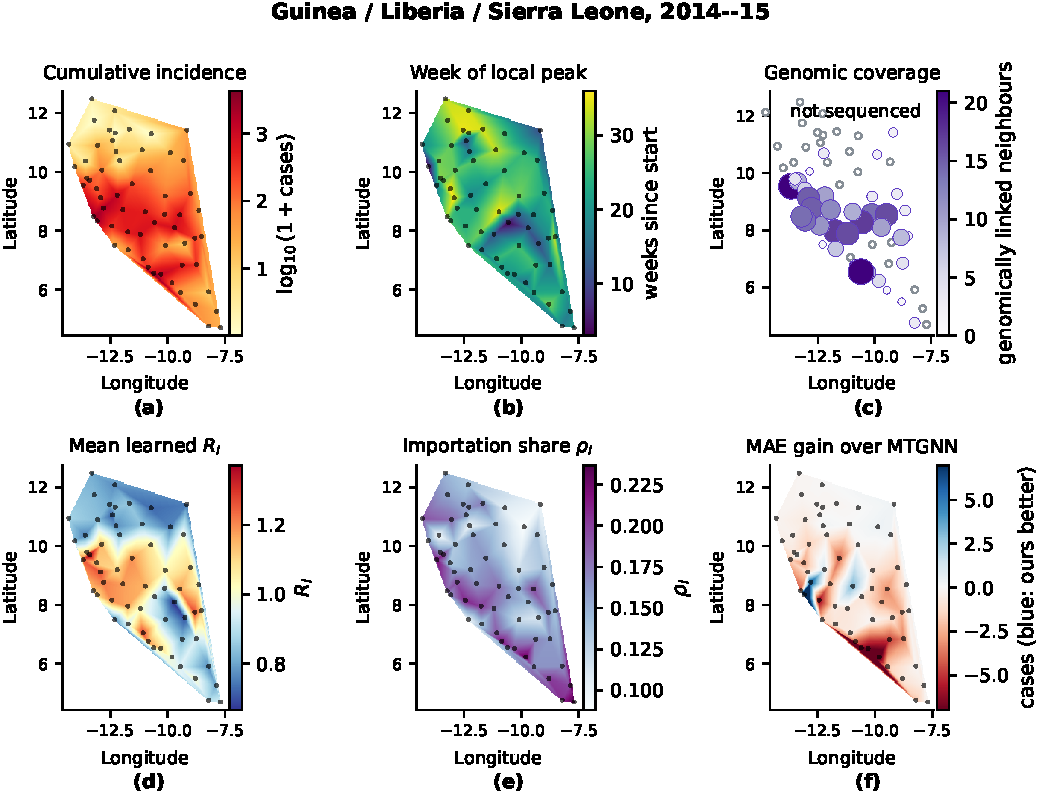
\includegraphics[width=0.495\textwidth]{figs/spatial_WA2014.pdf}\hfill
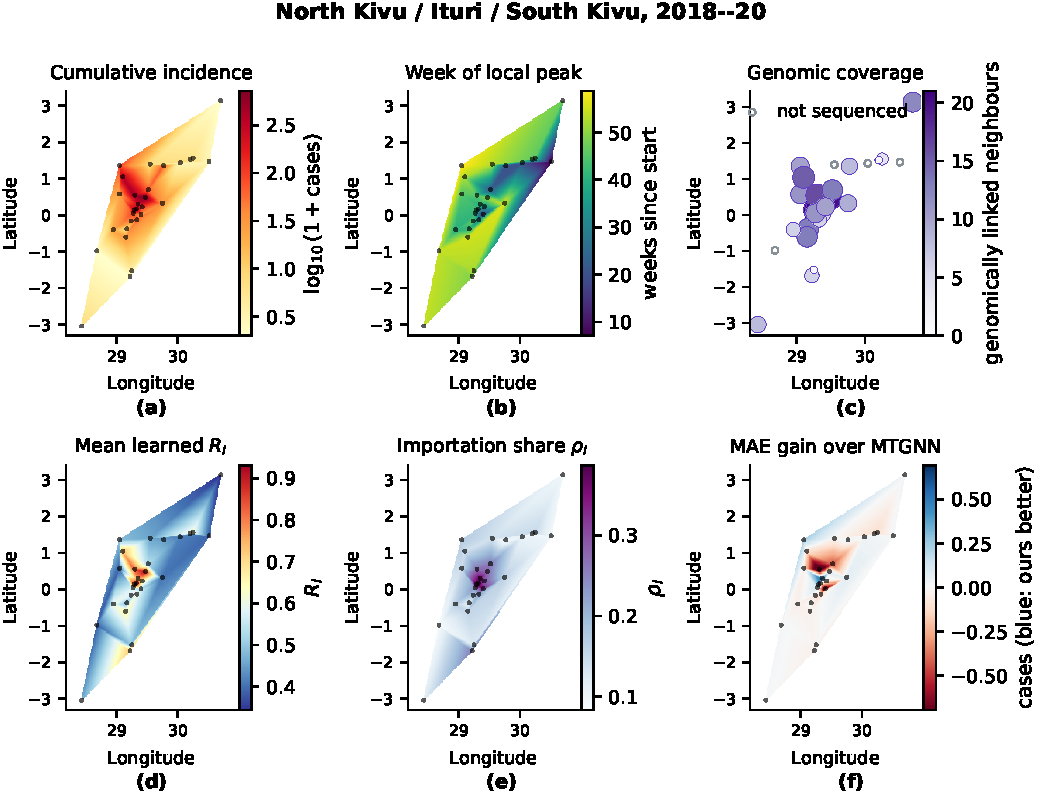
\includegraphics[width=0.495\textwidth]{figs/spatial_DRC1820.pdf}
\caption{Spatial structure of each outbreak and of the model's behaviour, interpolated over seat-town coordinates: (a)~cumulative incidence, (b)~week of the local peak, (c)~genomic coverage, (d)~mean learned $R_i$, (e)~importation share $\rho_i$ and (f)~MAE gain over MTGNN. Hollow markers in (c) are regions with no sequenced cases; blue in (f) is where RIG-Net-GI is more accurate.}
\label{fig:spatial}
\end{figure*}

\begin{figure*}[t]
\centering
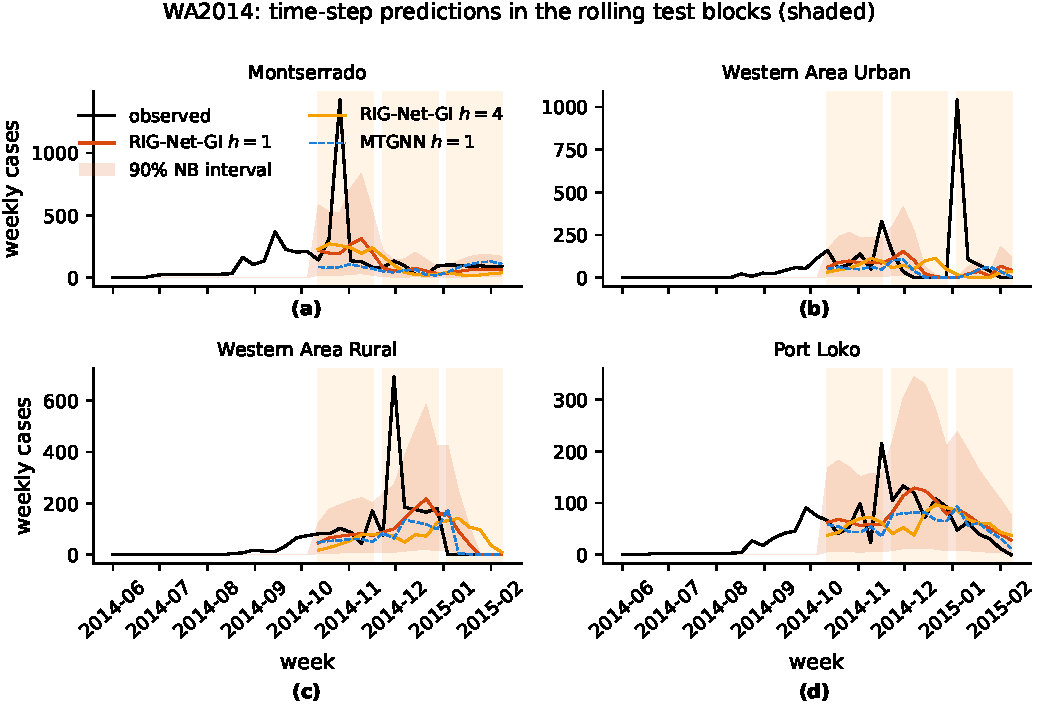
\includegraphics[width=0.495\textwidth]{figs/timestep_WA2014.pdf}\hfill
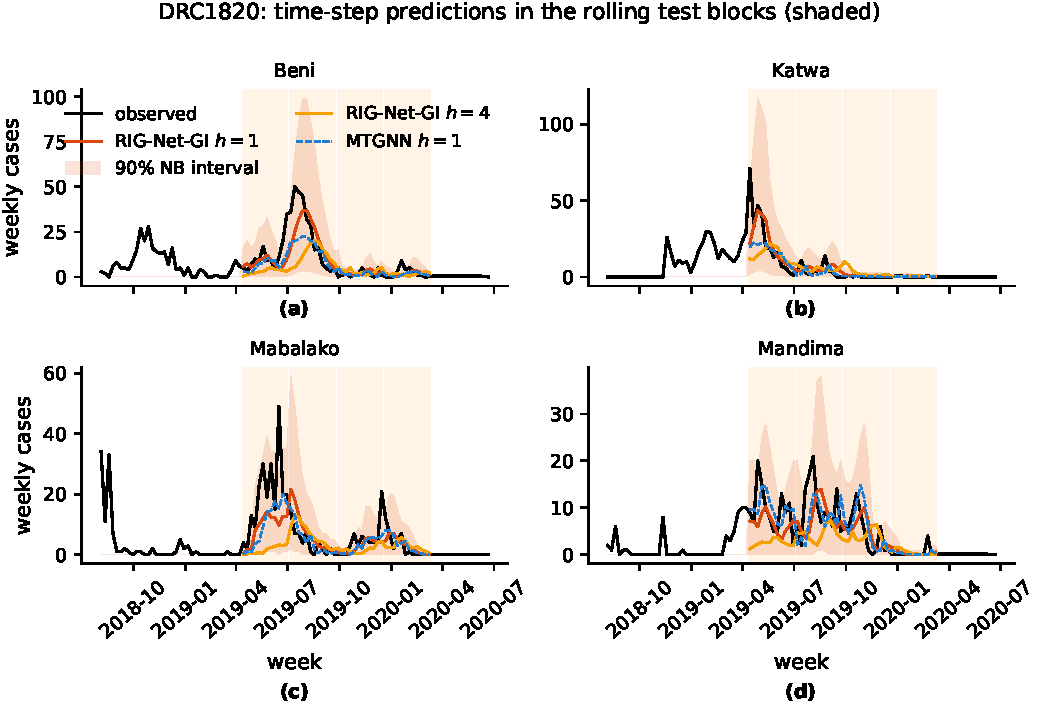
\includegraphics[width=0.495\textwidth]{figs/timestep_DRC1820.pdf}
\caption{Time-step predictions for the four highest-incidence regions of each panel, (a)--(d) in descending order of cumulative incidence; rolling test blocks shaded. Band is the 90\% negative-binomial interval at $h{=}1$.}
\label{fig:timestep}
\end{figure*}


\begin{figure*}[t]
\centering
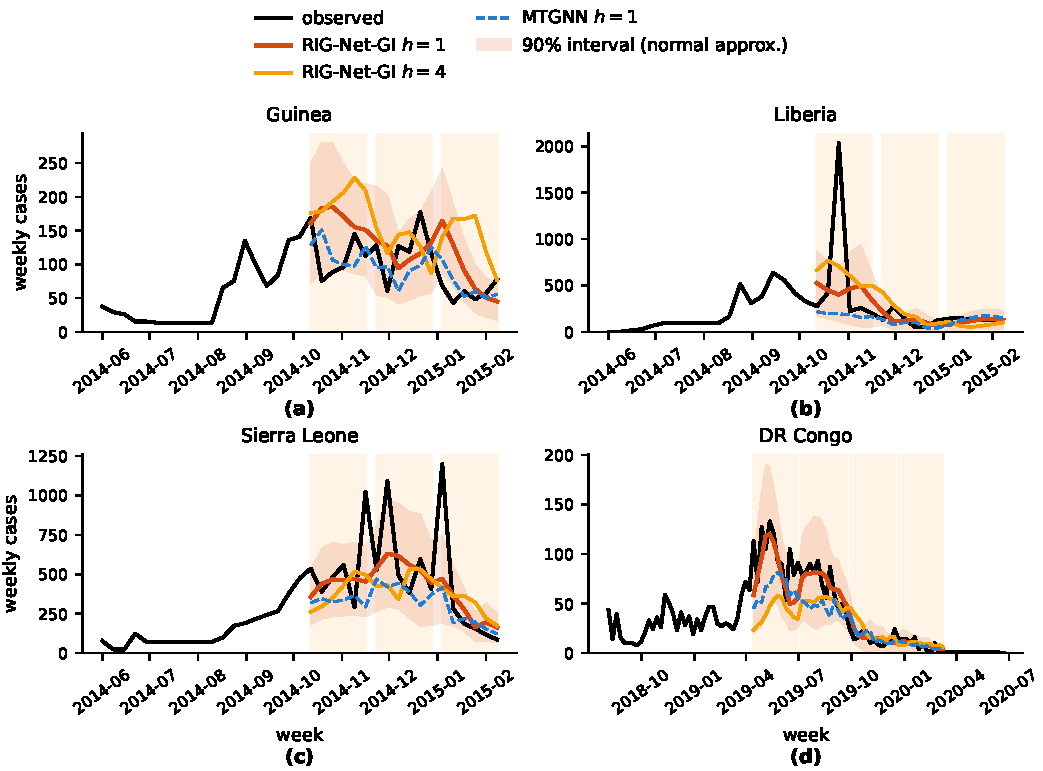
\includegraphics[width=\textwidth]{figs/timestep_countries.pdf}
\caption{National time-step predictions, aggregated from the region-level forecasts, for (a)~Guinea, (b)~Liberia, (c)~Sierra Leone and (d)~DR~Congo; test blocks shaded. The band is a normal approximation to the sum of the regional negative binomials, not an exact interval.}
\label{fig:countryts}
\end{figure*}

\subsection{RQ5: spatial and spatio-temporal structure}

\begin{figure*}[t]
\centering
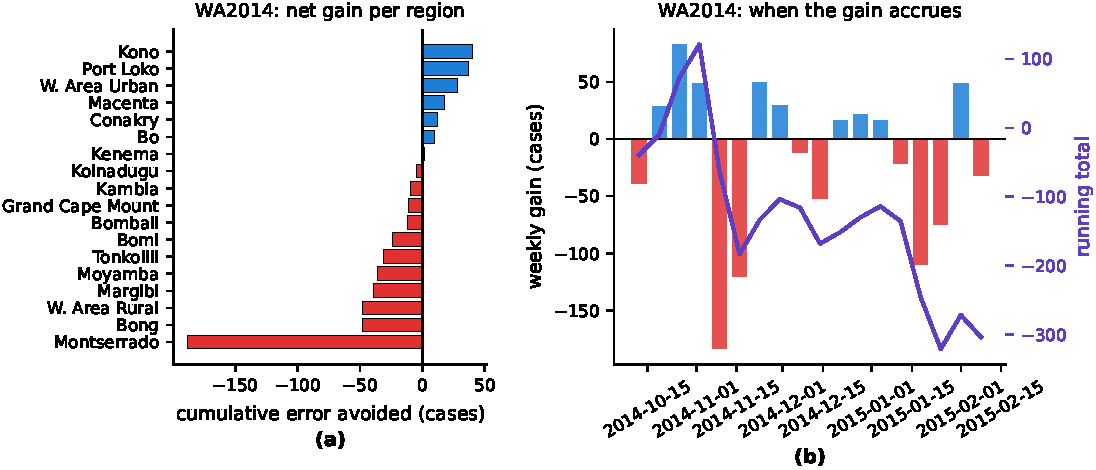
\includegraphics[width=\textwidth]{figs/sterr_WA2014.pdf}\\[4pt]
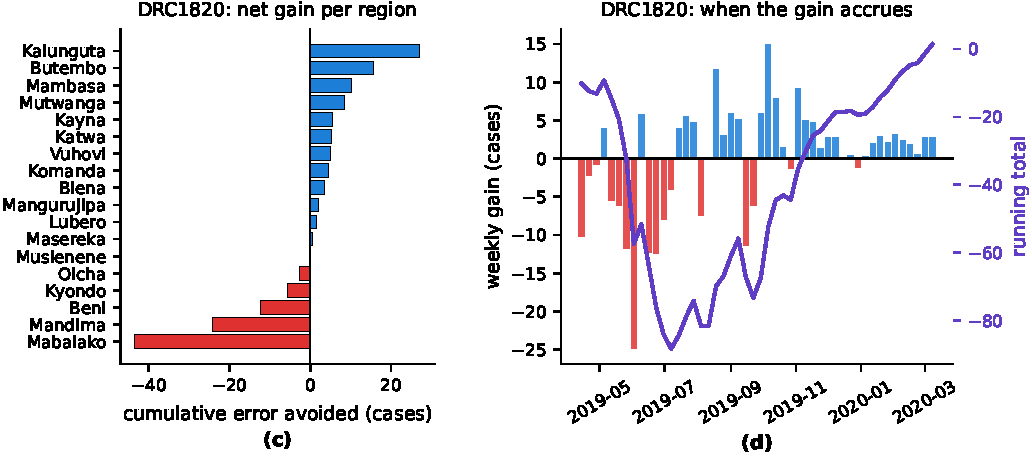
\includegraphics[width=\textwidth]{figs/sterr_DRC1820.pdf}
\caption{Where and when the 2-week-ahead gain over MTGNN accrues, for the highest-incidence regions; WA2014 in (a,b) and DRC1820 in (c,d). (a,c)~cumulative error avoided per region, blue where RIG-Net-GI is more accurate over the test blocks and red where it is worse. (b,d)~the same quantity summed over regions week by week (bars) with its running total (purple), so the sign and timing of the advantage are visible rather than averaged away.}
\label{fig:sterr}
\end{figure*}

\begin{figure}[t]
\centering
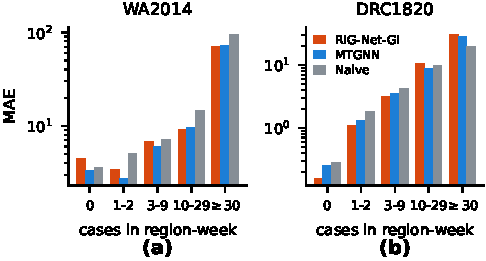
\includegraphics[width=\columnwidth]{figs/regime.pdf}
\caption{MAE stratified by the observed incidence of the region-week (log scale), for (a)~WA2014 and (b)~DRC1820.}
\label{fig:regime}
\end{figure}

Fig.~\ref{fig:spatial} places both outbreaks and the model's behaviour in space, interpolated over seat-town coordinates: cumulative incidence (a), week of local peak (b), genomic coverage (c), mean learned $R_i$ (d), importation share (e) and MAE gain over MTGNN at the 2-week horizon (f). Fig.~\ref{fig:spatial}(a,b) show the epidemic structure the model has to capture: the west-to-east sweep of West Africa and the compact Mabalako--Katwa corridor of North Kivu. Fig.~\ref{fig:spatial}(d,e) show that the learned reproduction number is spatially coherent and rank-correlates with log cumulative incidence at $\rho_s=0.68$ on both panels, while the importation share is highest in the peripheral regions that received introductions rather than in the epicentres. Fig.~\ref{fig:spatial}(f) maps where the model beats the strongest baseline. Fig.~\ref{fig:timestep} shows the corresponding weekly trajectories for the largest regions, with the observed series, the 1- and 4-week-ahead means and the 90\% negative-binomial interval; the decoder tracks declining chains closely and lags sharp turning points.

Fig.~\ref{fig:countryts} aggregates the same forecasts to the national level for all four countries. The national view separates two behaviours that the pooled metrics merge: on Sierra Leone and DR~Congo the model tracks the national curve more closely than MTGNN (169 vs 202 and 10.8 vs 18.9 weekly cases MAE), whereas on Guinea and Liberia it is worse (44 vs 32 and 176 vs 158), because both national curves contain single-week reporting spikes, the Montserrado backlog is visible as the isolated Liberian peak of October 2014, that a renewal rollout smooths through.

Pooled metrics hide where a model's advantage lies. Fig.~\ref{fig:sterr} decomposes the 2-week-ahead difference against the strongest baseline over 1{,}098 scored region-weeks on WA2014 and 1{,}392 on DRC1820, by region on the left and by week on the right. On DRC1820 it is better on average in 79\% of regions; its largest gains are in Kalunguta and the mid-2019 decline, and its largest loss is Mabalako, the epicentre during the growth phase. On WA2014 it is better on average in 43\% of regions, with Kono the largest gain and Montserrado, the county holding the October 2014 reporting backlog, the largest loss. The gains are therefore concentrated rather than uniform: a minority of region-weeks with large absolute errors drives the RMSE advantage, which is consistent with the MAE--RMSE split of RQ1.

Fig.~\ref{fig:regime} stratifies by incidence regime. On DRC1820 RIG-Net-GI has the lowest error in the three lowest bins (0.15 vs 0.25 for MTGNN in zero weeks) and is slightly worse in the $\geq30$ bin. On WA2014 the ordering reverses: it is best in the $\geq30$ bin (71.9 vs 73.2) and worst in the zero bin (4.22 vs 3.40). The renewal prior pays off where the epidemic curve has structure to extrapolate and costs a little where the right answer is simply zero.

\subsection{RQ6: are the learned quantities meaningful?}

\begin{figure*}[t]
\centering
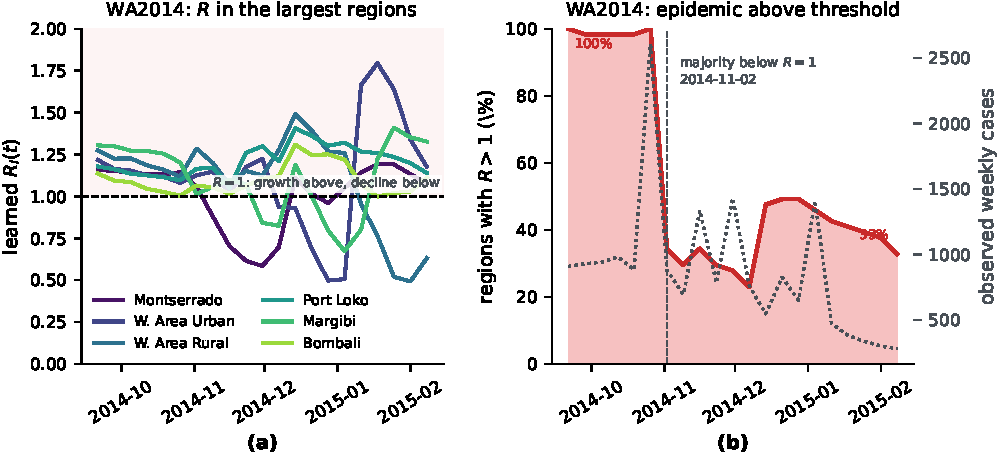
\includegraphics[width=\textwidth]{figs/Rfield_WA2014.pdf}\\[4pt]
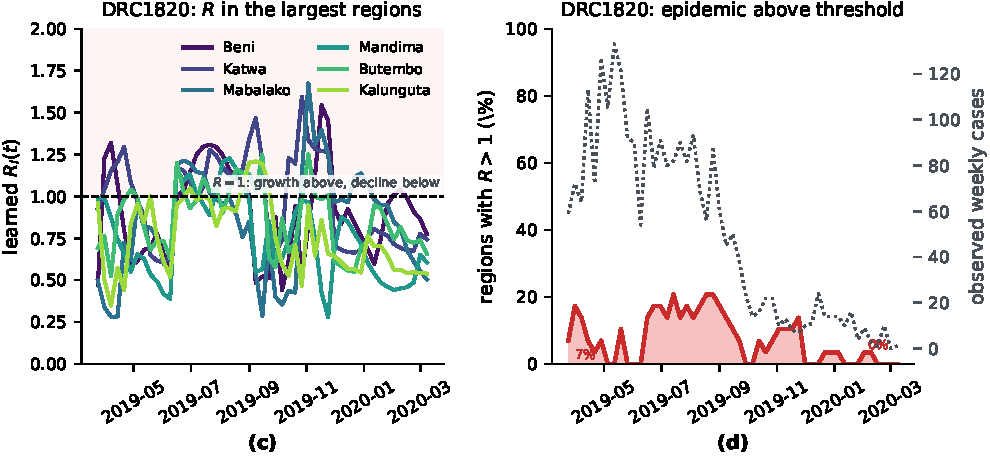
\includegraphics[width=\textwidth]{figs/Rfield_DRC1820.pdf}
\caption{The learned reproduction number through the test blocks, WA2014 in (a,b) and DRC1820 in (c,d). (a,c)~$R_i(t)$ for the six largest regions, with the supercritical half-plane above $R=1$ shaded. (b,d)~the share of regions with $R_i>1$ (red) against observed national incidence (dotted), with the first and last values marked and, on WA2014, the week the majority of regions fall below threshold; the crossing precedes the fall in the case curve.}
\label{fig:rfield}
\end{figure*}

\begin{figure*}[t]
\centering
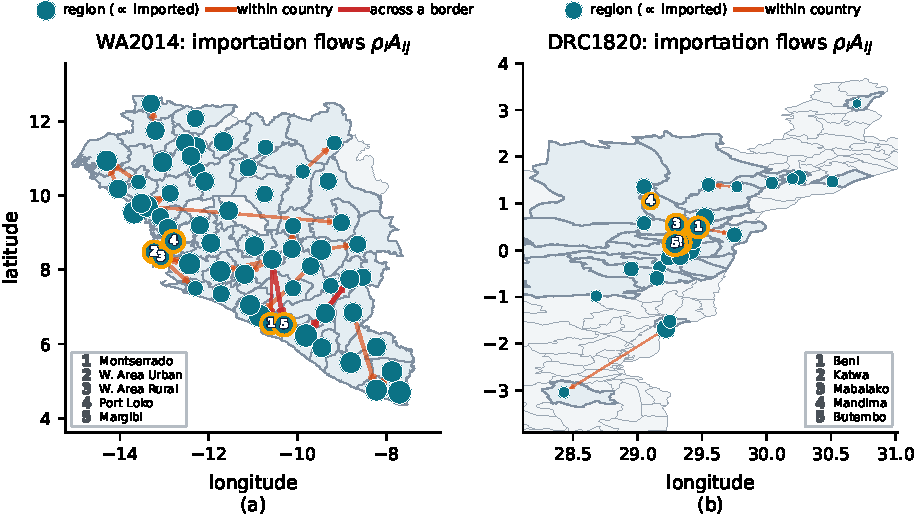
\includegraphics[width=\textwidth]{figs/flows.pdf}
\caption{Learned importation flows $\rho_i A_{ij}$ for (a)~WA2014 and (b)~DRC1820: the 28 strongest edges, with arrow width and head size proportional to the flow and cross-border flows in red. Marker area is the imported pressure a region receives, so sinks of importation are visible as well as sources. The five highest-incidence regions are numbered and named in the corner key.}
\label{fig:flows}
\end{figure*}

\begin{table}[t]
\caption{Learned quantities (mean over 5 seeds and all folds). $\beta_k$ is the suppression coefficient of response indicator $k$; the implied effect is the multiplicative reduction in $R$ per one-standard-deviation increase.}
\label{tab:interp}
\centering\footnotesize
\resizebox{\columnwidth}{!}{%
\begin{tabular}{lcc}
\toprule
Quantity & WA2014 & DRC1820 \\
\midrule
Gate weight: geographic & 0.468 & 0.671 \\
Gate weight: learned static & 0.100 & 0.118 \\
Gate weight: attention & 0.150 & 0.138 \\
Gate weight: \textbf{genomic} & \textbf{0.282} & \textbf{0.074} \\
\midrule
$\beta$: laboratory-confirmation share & 0.038 & 0.020 \\
$\beta$: surveillance load & \textbf{0.087} & 0.025 \\
$\beta$: response maturity & 0.019 & \textbf{0.040} \\
Implied max.\ $R$ reduction per s.d. & 8.4\% & 3.9\% \\
\midrule
Importation share $\rho_i$: mean (range) & 0.16 (0.09--0.24) & 0.19 (0.08--0.39) \\
Cross-border share of importation & 29\% &, \\
\bottomrule
\end{tabular}}

\end{table}

Table~\ref{tab:interp} reports the learned quantities and Figs.~\ref{fig:rfield}--\ref{fig:flows} their spatio-temporal structure. Three observations stand out.

First, the gate allocates 28\% of spatial mixing to the genomic graph on WA2014 but only 7\% on DRC1820, where geography dominates at 67\%. This matches the epidemiology: the West African epidemic was a multi-country event with long-range introductions that genomes resolve and distance does not, whereas the Nord Kivu outbreak remained spatially compact. Consistently, 29\% of the learned importation weight in WA2014 crosses a national border (Fig.~\ref{fig:flows}), concentrated on the Guinea--Sierra Leone and Liberia--Sierra Leone corridors and visible as the long west-to-east arrows; in DRC1820 the flows stay inside the North Kivu corridor.

Second, the learned $R$ (Fig.~\ref{fig:rfield}) reproduces the qualitative course of both outbreaks. On WA2014 every region starts the test period above one, the majority drops below threshold in the week of 2 November 2014, and the share falls to 33\% by February 2015, with a visible rebound in the Western Area in January; on DRC1820 only 7\% of zones begin above one and none end there, which is the signature of an outbreak already in retreat. The share crosses below half several weeks before the national case curve falls, so the quantity leads the counts it is computed from. RQ12 validates this field against an EpiEstim estimator and finds the agreement weak and the range strongly shrunk, so the field should be read as a spatially coherent forecasting parameter and not as an epidemiological estimate.

Third, the suppression coefficients are small but non-zero and select different indicators per panel: surveillance load on WA2014 ($\beta=0.087$, an 8.4\% reduction in $R$ per standard deviation) and response maturity on DRC1820 ($\beta=0.040$, 3.9\%). As an external check, surveillance load correlates $-0.36$ (WA2014) and $-0.42$ (DRC1820) with the empirical weekly growth rate, so the model selects the indicator carrying genuine signal. These are surveillance-derived proxies and the coefficients are not causal intervention effects; $\rho$ is additionally subject to Proposition~\ref{prop:ident}.

\subsection{RQ7: empirical validation of the theory}

\begin{figure*}[t]
\centering
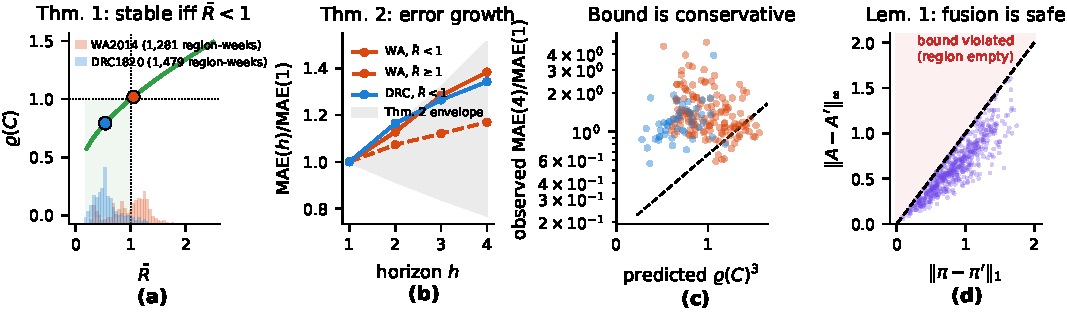
\includegraphics[width=\textwidth]{figs/theory.pdf}
\caption{Each theoretical result against the behaviour it governs. (a)~stability threshold, with the distribution of the learned $R$ over all 2{,}760 region-weeks beneath it and each panel's median on the curve; (b)~measured error growth by regime against the Theorem~\ref{thm:error} envelope; (c)~realised four-week amplification against the contraction factor, one point per region per test block ($n=195$, log scale); (d)~600 random gate pairs against the Lemma~\ref{lem:lip} bound.}
\label{fig:theory}
\end{figure*}

Theory is only useful if it binds on real data. Fig.~\ref{fig:theory} tests the three claims that drive the design.

First, Theorem~\ref{thm:contract} predicts stability exactly when $\bar R<1$. Fig.~\ref{fig:theory}(a) confirms the algebraic claim, the spectral radius of the companion matrix built from the Ebola generation interval crosses one at $\bar R=1.000$, and locates the model's operating point: the median learned $\bar R$ is $1.05$ on WA2014 and $0.54$ on DRC1820, so the DRC rollout sits well inside the contractive region while West Africa sits on the boundary. That difference alone predicts the stability gap between the two panels.

Second, Fig.~\ref{fig:theory}(b) tests the behavioural consequence on the forecasts. Splitting test weeks by the mean learned $\bar R$, error at four weeks is $1.17\times$ its one-week value in weeks with $\bar R<1$ on WA2014 but $1.38\times$ in weeks with $\bar R\geq1$; on DRC1820, where almost all test weeks have $\bar R<1$, growth is $1.34\times$. The measured curves lie inside the envelope and the two regimes separate in the predicted direction. This is the mechanism behind the phase dependence of RQ3, measured directly rather than inferred.

Third, Fig.~\ref{fig:theory}(c) asks whether the bound is usable \emph{operationally}, could a responder read $\bar R$ off the model and anticipate how much a four-week forecast will degrade? Here the answer is no, and we report it. Taking one point per region per test block gives 195 cases with enough signal to score. Realised amplification exceeds the pure contraction factor $\varrho(C)^3$ in 149 of them (76\%), and the two are not positively associated ($\rho_s=-0.07$, $n=195$). This does not contradict Theorem~\ref{thm:error}, whose bound also carries an additive parameter-error term; it shows that on these panels that additive term, not the contraction factor, dominates. The theory therefore explains the \emph{regime} dependence but does not give a usable per-block error forecast.

Finally, Lemma~\ref{lem:lip} bounds the sensitivity of the fused graph to the gate. Sampling 600 random gate pairs over the learned adjacencies, Fig.~\ref{fig:theory}(d) finds no violation of $\|A-A'\|_\infty\leq\|\pi-\pi'\|_1$, with the observed values typically a factor of two inside the bound. Adding the fourth, genomic channel therefore cannot destabilise message passing, which is what licenses using a sparse and partially observed graph as a prior.

\subsection{RQ8: what does the genomic prior encode?}

\begin{figure*}[t]
\centering
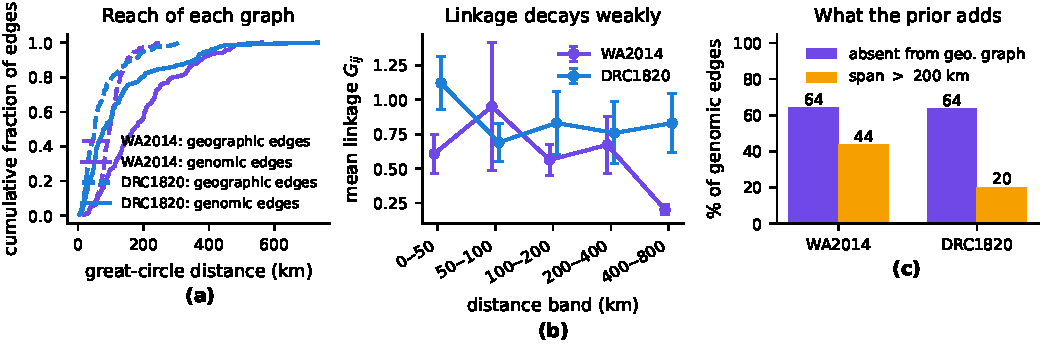
\includegraphics[width=\textwidth]{figs/genomic_validation.pdf}
\caption{What the genomic prior adds over the geographic kernel. (a)~distribution of edge lengths; (b)~mean linkage by distance band; (c)~share of genomic edges absent from the geographic graph and spanning more than \SI{200}{km}.}
\label{fig:genval}
\end{figure*}

If the genomic graph merely restated geography, it could not add information, and its 28\% gate weight on WA2014 would be redundant. We test this three ways. In Fig.~\ref{fig:genval}(a) genomic edges are solid and the six-nearest-neighbour geographic edges dashed. First, the two graphs reach different distances: the median genomic edge spans \SI{172}{km} on WA2014 against \SI{96}{km} for the geographic graph, and \SI{82}{km} against \SI{51}{km} on DRC1820, and Fig.~\ref{fig:genval}(a) shows the gap holds across the whole distribution rather than at a few outliers. Second, linkage strength decays only weakly with distance (rank correlation $-0.23$ on WA2014, $-0.12$ on DRC1820) and on DRC1820 the binned means in Fig.~\ref{fig:genval}(b) are flat within error, so distance cannot stand in for linkage. Third, and most directly, 64\% of genomic edges on both panels connect regions that are \emph{not} adjacent in the geographic graph, and 44\% of West African genomic edges span more than \SI{200}{km} (Fig.~\ref{fig:genval}(c)). These are the cross-border introductions that drove the multi-country epidemic. Linkage is also nearly uncorrelated with simple co-activity ($\rho_s=0.01$ on WA2014, $0.13$ on DRC1820), so it is not a proxy for two regions happening to have cases at the same time. Genomic coverage is itself partial, 37 of 61 WA2014 regions and 24 of 29 DRC1820 health zones have sequenced cases before the last cut-off, which is why the gate masks the genomic row for unsequenced regions rather than imputing it.

\subsection{RQ9: calibration and scale-free metrics}

\begin{table}[t]
\caption{Scale-free accuracy, peak-timing error and, for the probabilistic model, calibration. MASE is relative to a one-step naive forecast; peak-week error is the mean absolute difference between predicted and observed week of local maximum over regions with more than 20 cases. Within each column of a panel, \textbf{best}, \underline{second} and \uuline{third} are marked; our model is listed last.}
\label{tab:extra}
\centering\footnotesize
\resizebox{\columnwidth}{!}{%
\begin{tabular}{llccc}
\toprule
Panel & Model & MASE & sMAPE (\%) & Peak-week err. \\
\midrule
\multirow{5}{*}{WA2014}
 & MTGNN & \textbf{1.395} & 65.7 & 2.95 \\
 & N-BEATS & \underline{1.432} & 66.0 & \uuline{2.87} \\
 & EpiGNN & 1.472 & \uuline{65.2} & \underline{2.80} \\
 & Naive (ref.) & 1.809 & \textbf{37.3} & \textbf{1.00} \\
 & \textbf{RIG-Net-GI (ours)} & \uuline{1.440} & \underline{50.1} & 3.36 \\
\midrule
\multirow{5}{*}{DRC1820}
 & MTGNN & \underline{1.566} & 83.8 & 3.13 \\
 & N-BEATS & 1.585 & \uuline{83.1} & 2.33 \\
 & EpiGNN & \uuline{1.576} & 83.1 & \underline{1.20} \\
 & Naive (ref.) & 1.720 & \textbf{23.1} & \textbf{1.00} \\
 & \textbf{RIG-Net-GI (ours)} & \textbf{1.491} & \underline{24.4} & \uuline{1.93} \\
\midrule
\multicolumn{5}{l}{\emph{Probabilistic (RIG-Net-GI only; baselines are point forecasts)}}\\
WA2014 & 90\% interval coverage & \multicolumn{3}{c}{88.0\% \quad (WIS 9.27)} \\
DRC1820 & 90\% interval coverage & \multicolumn{3}{c}{93.9\% \quad (WIS 1.00)} \\
\bottomrule
\end{tabular}}

\end{table}

Table~\ref{tab:extra} reports metrics that do not reward simply predicting small numbers. On MASE, RIG-Net-GI is best on DRC1820 (1.491 vs 1.566) and slightly behind MTGNN on WA2014. On sMAPE, which weights proportional error, the margin is large on both panels (24.4\% vs 83.8\% on DRC1820), because the renewal decoder tracks small persistent chains that the baselines over-smooth to near zero. The naive forecast scores well on sMAPE for the same reason it scores well nowhere else: repeating last week is proportionally accurate in a long tail of unchanged region-weeks.

Peak-week timing is a negative result and we report it as such: RIG-Net-GI is the \emph{worst} of the learned models at locating the week of a local peak on WA2014 (3.36 weeks vs 2.80 for EpiGNN). This is the growth-phase weakness of RQ3 seen in a different metric, a momentum-carrying decoder lags turning points, and the naive forecast trivially wins this metric by construction.

The negative-binomial head is well calibrated without any post-hoc adjustment: nominal 90\% predictive intervals contain 88.0\% of held-out observations on WA2014 and 93.9\% on DRC1820. This matters operationally, because an interval is what a response team can act on, and none of the 15 point-forecasting baselines provides one.

\subsection{RQ10: the four-country health-access and sequencing nexus}

\begin{figure*}[t]
\centering
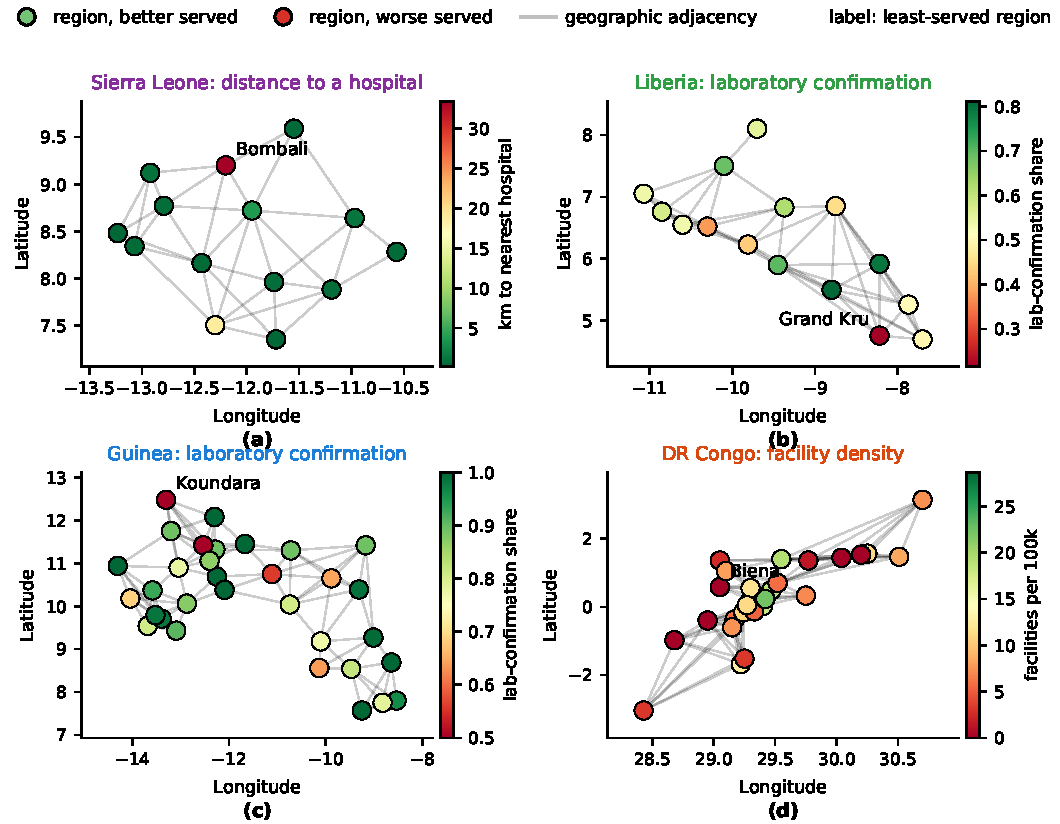
\includegraphics[width=\textwidth]{figs/nexus.pdf}
\caption{Health-access nexus over the model's region graph, for (a)~Sierra Leone, (b)~Liberia, (c)~Guinea and (d)~DR~Congo; nodes are regions, edges the geographic adjacency, colour the access indicator named in each title, whose definition differs by country but whose direction is common: green is better served, red worse. The least-served region of each country is labelled.}
\label{fig:nexus}
\end{figure*}

\begin{figure*}[t]
\centering
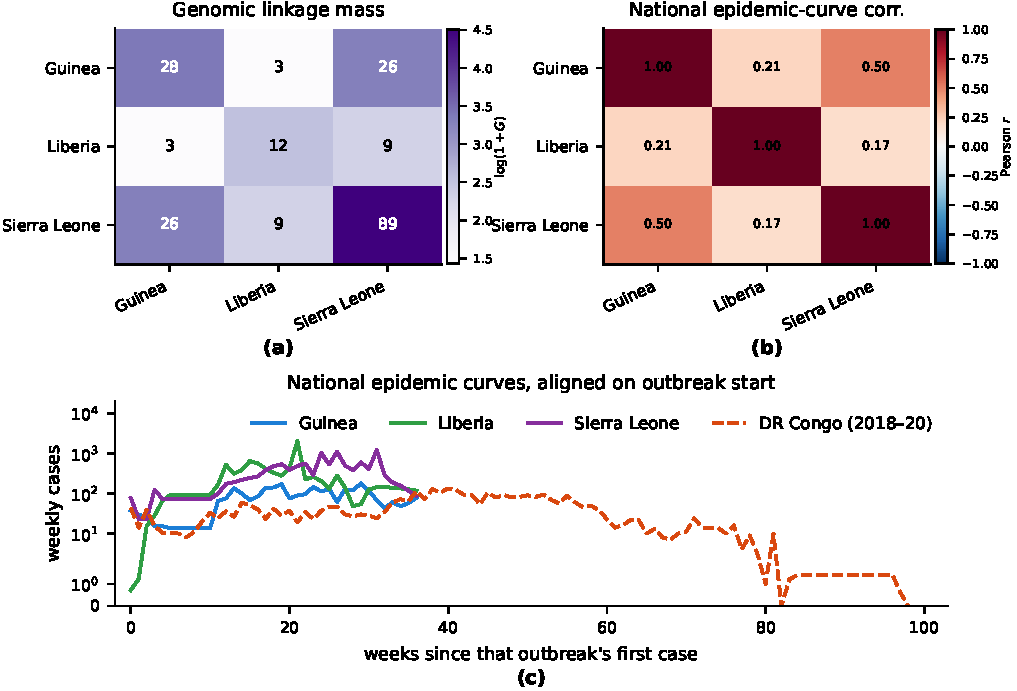
\includegraphics[width=\textwidth]{figs/countries.pdf}
\caption{Relationships between the national epidemics. (a)~genomic linkage mass within and between countries; (b)~correlation between national weekly curves; (c)~national incidence aligned on each outbreak's first reported case.}
\label{fig:countries}
\end{figure*}

\begin{figure*}[t]
\centering
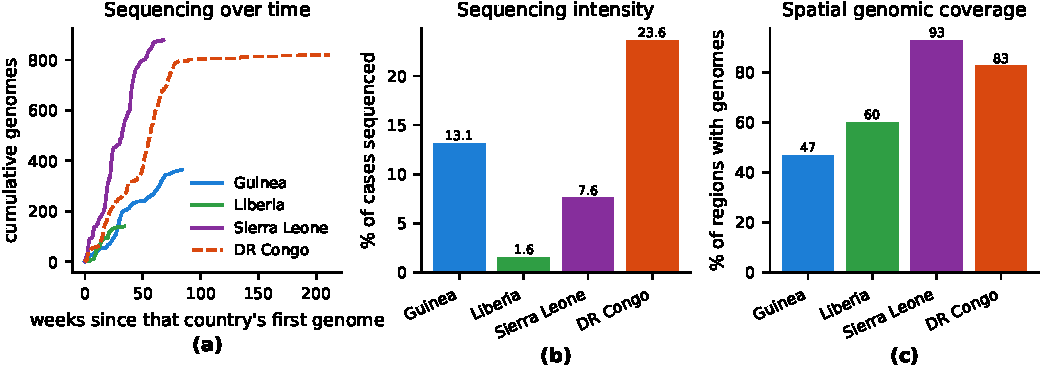
\includegraphics[width=\textwidth]{figs/sequencing.pdf}
\caption{Genomic surveillance by country: (a)~cumulative genomes, (b)~genomes as a percentage of reported cases, (c)~percentage of regions with at least one sequenced case.}
\label{fig:seq}
\end{figure*}

The four countries differ sharply in both health-system access and genomic surveillance, and both differences bear on the model.

\textbf{Access.} Fig.~\ref{fig:nexus} maps the access indicator on the model's own region graph. Provenance differs by country and we do not smooth over it: Sierra Leone uses distance from the district seat to the nearest of 34 geolocated hospitals (national DHIS list, 1{,}099 facilities); DR~Congo uses healthsites.io counts per WorldPop population; Liberia and Guinea have no obtainable geolocated facility list and use the laboratory-confirmation share instead. In Sierra Leone, referral access is uneven: the median district seat is within \SI{0.7}{km} of a hospital but Bonthe is \SI{33}{km} away. In DR~Congo, facility provision ranges from zero to 28.7 facilities per 100k across health zones. For Liberia and Guinea no geolocated facility list could be obtained, so we substitute the laboratory-confirmation share, and we flag this as a weaker, differently-constructed indicator rather than presenting the four panels as comparable. Access correlates with forecast error only in DR~Congo ($\rho_s=0.43$ between facilities per 100k and 2-week MAE) and not in Sierra Leone ($\rho_s=0.03$); the DRC association is confounded by incidence, since well-served zones are also the epicentres, so we do not read it causally.

\textbf{Cross-country structure.} Fig.~\ref{fig:countries} shows that 37\% of genomic linkage mass in West Africa is off-diagonal, that is cross-border, with the strongest coupling between Guinea and Sierra Leone (28 units) and the weakest between Guinea and Liberia (3). National epidemic curves are only moderately correlated (Guinea--Sierra Leone $r=0.50$, Liberia--Sierra Leone $r=0.17$), so the genomic coupling is not simply a restatement of synchronised national curves. This is the multi-country structure that the genomic channel supplies and a distance kernel cannot, and it is why the gate assigns that channel 28\% weight on WA2014 against 7\% on the spatially compact DRC panel.

\textbf{Sequencing.} Fig.~\ref{fig:seq} quantifies the surveillance asymmetry, where Fig.~\ref{fig:seq}(c) is the fraction of rows for which the genomic channel of the gate is unmasked: DR~Congo sequenced 23.6\% of reported cases, Guinea 13.1\%, Sierra Leone 7.6\% and Liberia only 1.6\%. Spatial coverage follows a different ordering, 93\% of Sierra Leonean districts have at least one genome against 47\% of Guinean prefectures, and it is spatial coverage, not sequencing intensity, that determines how many rows of the genomic adjacency are usable. Liberia is the limiting case: 140 genomes over 15 counties, which is why several Liberian rows remain masked and why the genomic prior helps least there. A practical implication for outbreak genomics is that for a model of this kind, sequencing breadth across regions is worth more than depth within the epicentre.


\begin{figure*}[t]
\centering
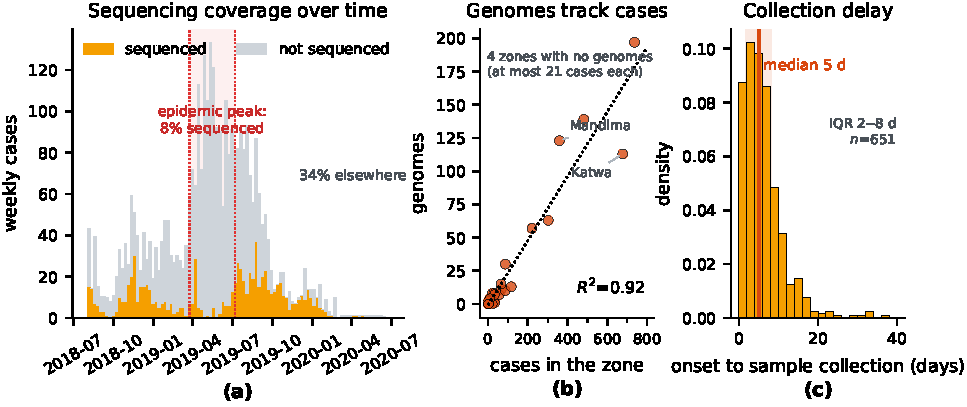
\includegraphics[width=\textwidth]{figs/seqintegration.pdf}
\caption{How sequencing was integrated into the DRC1820 response. (a)~weekly cases split into those with and without a genome, by sample collection date; the shaded band is the epidemic peak, over which coverage falls to 8\% against 34\% in the rest of the outbreak. (b)~genomes against cases per health zone, with the least-squares fit and the largest residual on either side named; the proportionality is what the $\sqrt{n_in_j}$ normalisation of~\eqref{eq:gen} assumes. (c)~the one delay the public metadata supports, symptom onset to sample collection, with the interquartile range shaded. Sequencing and release dates are not published, so the later steps of the sample-to-sequence pipeline cannot be measured and are not shown.}
\label{fig:seqint}
\end{figure*}

\subsection{RQ10b: when and where were genomes actually produced?}

A genomic prior is only as useful as the sequencing behind it, so Fig.~\ref{fig:seqint} asks what that sequencing looked like on DRC1820. Three things follow. First, 23\% of reported cases have a genome, but coverage is far from uniform in time: over the March--July 2019 peak, which carries 1{,}457 of the 3{,}466 cases, only 8\% were sequenced against 34\% in the rest of the outbreak, collection fell to between zero and five genomes a week, and the single largest week has none at all. This is the period of the Katwa and Butembo attacks on the response, and it means the prior is thinnest exactly when the epidemic is largest, which is a structural limitation of the channel rather than of our use of it.

Second, across health zones genomes are close to proportional to cases ($R^2=0.92$, 25 of 29 zones sequenced). That is what~\eqref{eq:gen} assumes when it normalises linkage counts by $\sqrt{n_in_j}$, so the assumption is supported here. The residuals are informative where they are large: Katwa, the second-worst affected zone, is the most under-sequenced relative to its case load (678 cases, 113 genomes), while Mandima is the most over-sequenced. The four zones with no genomes at all have at most 21 cases each, so they are missing for reasons unrelated to their case load, which is why the gate masks them rather than treating their rows as empty.

Third, the measurable delay is short: a median of five days from symptom onset to sample collection (IQR 2--8, $n=651$). The delays that matter operationally also include sequencing and release, which the published metadata does not record, so we cannot measure the full sample-to-sequence lag and do not estimate it. This matters for deployment: our leakage-safe design uses genomes collected before the forecast origin, but a real-time system would have access only to genomes \emph{released} by then, and that gap is unquantified here.

\subsection{RQ11: training dynamics}

\begin{figure*}[t]
\centering
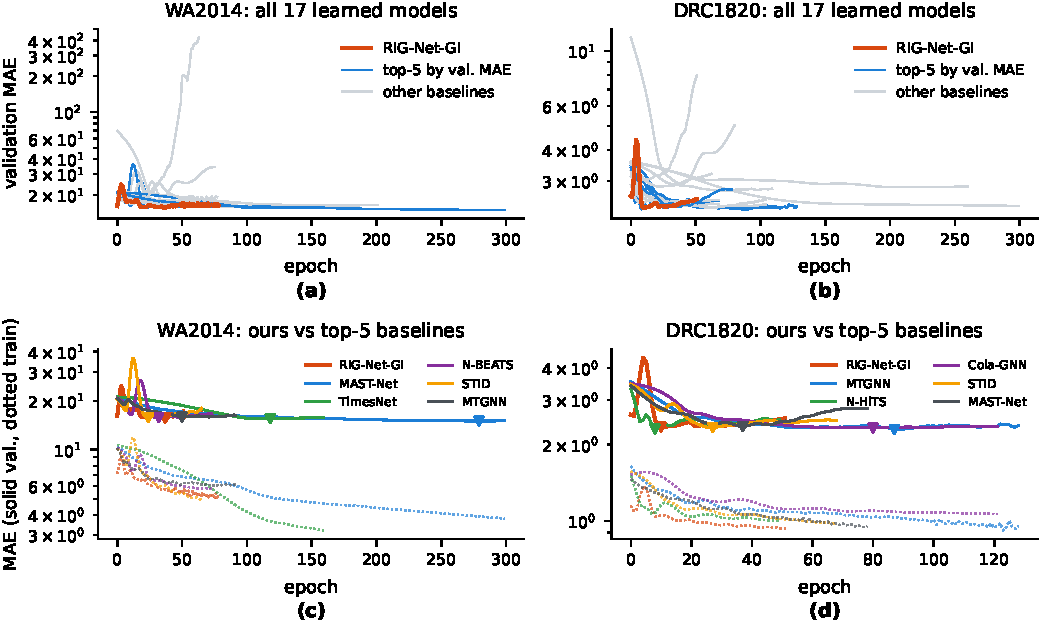
\includegraphics[width=\textwidth]{figs/training.pdf}
\caption{Training dynamics on the middle test block of each panel, seed 0, under the shared protocol. (a,b)~validation MAE for all 17 learned models, WA2014 then DRC1820. (c,d)~RIG-Net-GI against five strong baselines, MAST-Net among them, on the same two datasets, with validation (solid), training (dotted) and the selected epoch (triangles).}
\label{fig:training}
\end{figure*}

\begin{table}[t]
\caption{Convergence under the shared protocol (middle fold, seed 0): best validation MAE, the epoch at which it occurred, and wall-clock seconds on one CPU core. Rows are ordered by mean rank of best validation MAE across the two panels, with our model last; within each validation-MAE column, \textbf{best}, \underline{second} and \uuline{third} are marked.}
\label{tab:train}
\centering\footnotesize
\resizebox{\columnwidth}{!}{%
\begin{tabular}{lcccccc}
\toprule
\multirow{2}{*}{Model} & \multicolumn{3}{c}{WA2014} & \multicolumn{3}{c}{DRC1820} \\
\cmidrule(lr){2-4}\cmidrule(lr){5-7}
 & val.\ MAE & epoch & s & val.\ MAE & epoch & s \\
\midrule
MTGNN & 15.86 & 50 & 2.6 & \textbf{2.29} & 87 & 4.0 \\
STID & 15.76 & 24 & 0.7 & 2.33 & 27 & 0.7 \\
Cola-GNN & 15.97 & 98 & 4.6 & \uuline{2.32} & 80 & 2.9 \\
N-HiTS & 16.25 & 27 & 0.6 & \underline{2.30} & 8 & 0.5 \\
N-BEATS & 15.72 & 32 & 0.6 & 2.36 & 27 & 0.6 \\
TimesNet & \underline{15.50} & 118 & 2.1 & 2.84 & 21 & 1.0 \\
DLinear & 16.14 & 150 & 0.8 & 2.38 & 299 & 1.1 \\
STAEformer & 16.53 & 36 & 10.2 & 2.34 & 63 & 12.4 \\
EpiGNN & 16.30 & 51 & 1.5 & 2.36 & 63 & 1.5 \\
iTransformer & 16.90 & 12 & 1.4 & 2.44 & 8 & 1.1 \\
MAST-Net & \textbf{15.01} & 279 & 26.0 & 2.36 & 37 & 6.6 \\
AGCRN & 16.37 & 160 & 13.8 & 2.83 & 219 & 13.0 \\
PatchTST & 17.46 & 7 & 3.7 & 2.46 & 27 & 5.7 \\
TSMixer & 18.11 & 19 & 0.4 & 2.74 & 68 & 0.8 \\
MepoGNN & 19.33 & 34 & 1.1 & 2.93 & 39 & 1.3 \\
Autoformer & 19.50 & 22 & 0.6 & 3.03 & 10 & 0.5 \\
\midrule
\textbf{RIG-Net-GI (ours)} & \uuline{15.62} & 37 & 4.5 & 2.34 & 10 & 2.6 \\
\bottomrule
\end{tabular}}

\end{table}

Fig.~\ref{fig:training} and Table~\ref{tab:train} record what happens during fitting, which pooled test metrics cannot show. All models use the identical protocol: Adam, full batch, at most 300 epochs, early stopping on validation MAE with patience 40. Four observations.

First, several baselines \emph{diverge} on these panels. The grey curves rising by one to two orders of magnitude in the top-left panel are models whose validation error grows steadily after a few dozen epochs; early stopping rescues their reported scores, but the behaviour indicates the architectures are poorly matched to 9--32 training windows. AGCRN and DLinear run to 160--299 epochs before their best epoch, two of the slowest to settle.

Second, RIG-Net-GI converges early and stays flat: its best epoch is 37 on WA2014 and 10 on DRC1820, against 87 and 160--219 for MTGNN and AGCRN. The renewal decoder restricts the function class, the network predicts $R$, $\rho$ and $\iota$ rather than arbitrary counts, so there is less to fit.

Third, the train--validation gap, visible as the distance between dotted and solid curves in the bottom row, is smallest for RIG-Net-GI and widest for TimesNet, whose training MAE falls to roughly a third of its validation MAE on WA2014 while validation stalls. That is the classic overfitting signature on a small panel and is consistent with TimesNet's poor DRC1820 test result despite the best WA2014 validation score in this fold.

Fourth, the ordering by \emph{validation} MAE in Table~\ref{tab:train} is not the ordering by test MAE in Table~\ref{tab:main}: TimesNet has the best WA2014 validation score here yet ranks twelfth on test. This is the transfer failure quantified in RQ4, visible now at the level of a single training run.

\subsection{RQ12: leakage, validation of $R$, and calibration}

\begin{figure*}[t]
\centering
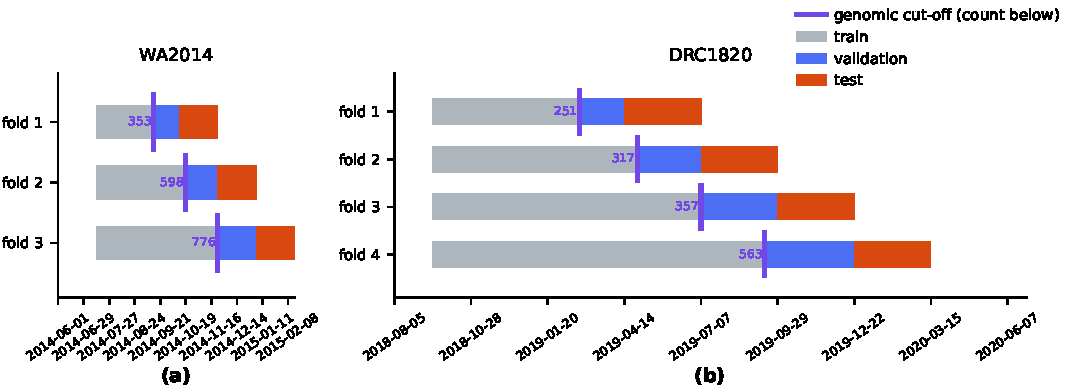
\includegraphics[width=\textwidth]{figs/leakage.pdf}
\caption{Rolling-origin folds for (a)~WA2014 and (b)~DRC1820, with the genomic cut-off marked (purple, with the genome count available at that point).}
\label{fig:leak}
\end{figure*}

\begin{figure*}[t]
\centering
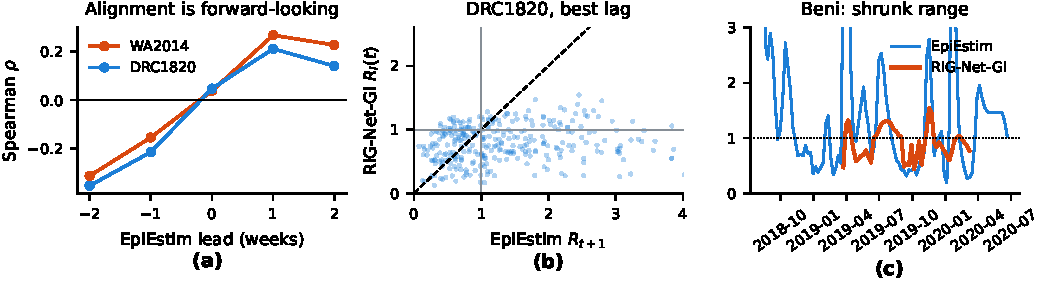
\includegraphics[width=\textwidth]{figs/epiestim.pdf}
\caption{The learned $R_i(t)$ against an EpiEstim-style estimator~\cite{cori2013} on the same generation interval: (a)~rank correlation by lead, (b)~scatter at the best lead, (c)~an example trajectory.}
\label{fig:epiestim}
\end{figure*}

\begin{figure}[t]
\centering
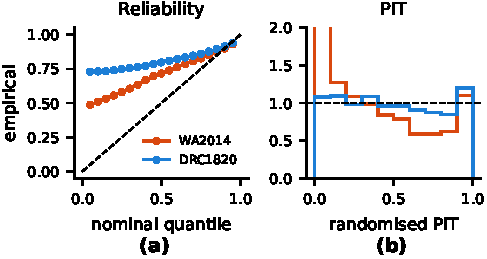
\includegraphics[width=\columnwidth]{figs/calibration.pdf}
\caption{Calibration of the negative-binomial head: (a)~reliability curve and (b)~randomised PIT, the appropriate diagnostic for counts.}
\label{fig:calib}
\end{figure}

\textbf{Leakage.} Using genomes as a forecasting prior creates an exposure that retrospective phylodynamics does not have, so we make the construction auditable. Fig.~\ref{fig:leak} places every fold on the calendar with its genomic cut-off, which sits at the end of that fold's training window. Between 353 and 776 West African genomes and 251 to 563 Nord Kivu genomes precede the respective cut-offs, and nothing sampled during or after a validation or test block enters the graph used to forecast it. The same applies to the case data, the scaler and the standardisation of the response indicators.

\textbf{Is the learned $R$ a reproduction number?} We compare against an EpiEstim-style estimator~\cite{cori2013} built from the same generation interval (Fig.~\ref{fig:epiestim}). Three findings, and the second is negative. First, the alignment is coherent and forward-looking: rank correlation is negative when EpiEstim is lagged, crosses zero at simultaneous alignment, and peaks at a one-week \emph{lead} ($\rho_s=0.27$ on WA2014, $0.21$ on DRC1820), which is exactly the quantity a one-week-ahead forecaster should encode. Second, the association is nonetheless weak, and the direction of movement agrees only 63\% (WA2014) and 55\% (DRC1820) of the time on the key question of whether $R$ is above or below one. Third, the learned $R$ is heavily shrunk: its 5th--95th percentile range is $0.34$--$1.44$ on WA2014 against $0.14$--$6.63$ for EpiEstim.

We therefore correct an interpretation that an earlier reading of our own results would have supported. The learned $R_i(t)$ is a \emph{regularised forecasting parameter} that behaves like a strongly shrunk, one-week-ahead reproduction number; it is spatially coherent and it drives the mechanism, but it is not an epidemiological estimate and should not be reported to responders as one. The quantities that survive as descriptive outputs are the gate weights and the importation share, which are structural rather than inferential.

\textbf{Calibration.} Fig.~\ref{fig:calib} replaces the single coverage number of RQ9 with the full diagnostic. The reliability curve sits above the diagonal at low quantiles because the predictive quantile is zero for a majority of region-weeks, which is the expected consequence of a point mass at zero in a discrete predictive distribution rather than a defect. The randomised PIT, which is the correct diagnostic for counts, is close to uniform on DRC1820 (Kolmogorov--Smirnov distance $0.029$) but shows mass near zero on WA2014 ($0.151$), meaning the model over-predicts in a substantial minority of West African region-weeks. The 90\% interval coverage reported earlier (88.0\% and 93.9\%) is therefore accurate at that level but hides a one-sided miscalibration on WA2014.

\begin{figure*}[t]
\centering
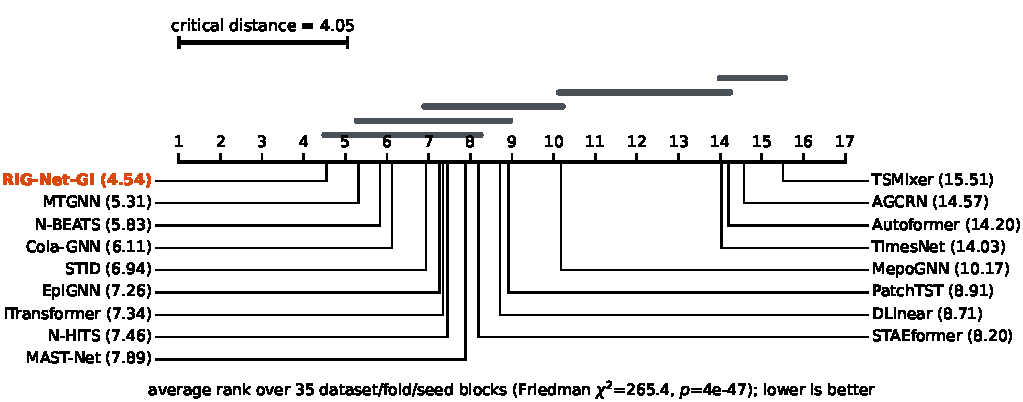
\includegraphics[width=\textwidth]{figs/cd.pdf}
\caption{Critical-difference diagram over 35 dataset--fold--seed blocks. Lower average rank is better; models joined by a bar are not significantly different.}
\label{fig:cd}
\end{figure*}

\begin{figure*}[t]
\centering
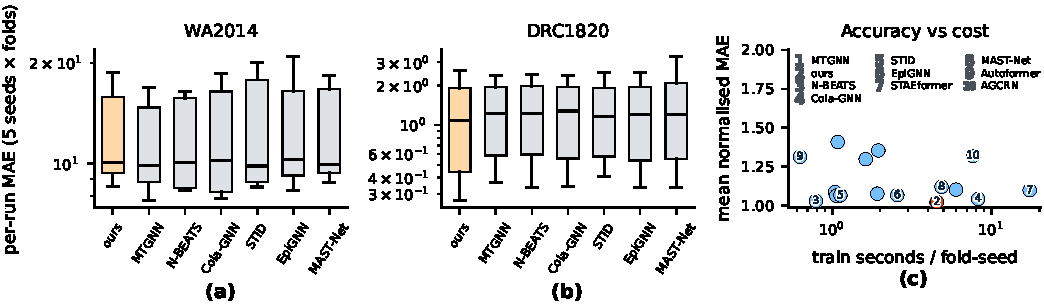
\includegraphics[width=\textwidth]{figs/variability.pdf}
\caption{(a,b)~per-run MAE over five seeds and all folds for the six best-ranked models plus MAST-Net, on WA2014 and DRC1820. (c)~accuracy against training cost, MAE normalised by the best value on each panel.}
\label{fig:variability}
\end{figure*}

\textbf{Multiple comparisons.} The pairwise Diebold--Mariano tests of RQ1 do not correct for 15 comparisons. Fig.~\ref{fig:cd} adds the standard alternative: a Friedman test over 35 dataset--fold--seed blocks followed by a Nemenyi post-hoc. The Friedman test rejects equality decisively, RIG-Net-GI obtains the best average rank (4.54, against 5.31 for MTGNN and 5.83 for N-BEATS), but the Nemenyi critical distance of 4.05 over 35 blocks is wide enough that the ten leading models, MTGNN, N-BEATS, Cola-GNN, STID, EpiGNN, iTransformer, N-HiTS, MAST-Net and STAEformer with ours, form a single indistinguishable group. This is the more conservative reading of our headline result and we adopt it: on 35 blocks, RIG-Net-GI ranks first by average rank but cannot be declared significantly better than the strongest baselines. Fig.~\ref{fig:variability} shows why: the per-run spread within a model, over five seeds and all folds, is of the same order as the gap between the leading models.

\subsection{RQ13: sensitivity, graph construction and cost}

\begin{figure}[t]
\centering
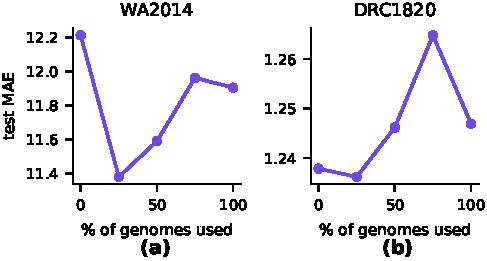
\includegraphics[width=\columnwidth]{figs/dose.pdf}
\caption{Genomic dose--response on (a)~WA2014 and (b)~DRC1820: test MAE when the linkage graph is built from a random subsample of the genomes; 0\% is the ablation without the prior.}
\label{fig:dose}
\end{figure}

\textbf{Genomic dose--response.} A natural objection is that the genomic gain reflects extra data rather than genomic structure. Fig.~\ref{fig:dose} subsamples the genomes. On WA2014, where 0\% denotes the ablation without the prior, the error falls from 12.07 to 11.24 with only 25\% of genomes, and does not improve further with 50\%, 75\% or 100\% (11.68, 11.70, 11.66); a sparse but spatially broad sample is sufficient, which is the same conclusion reached from the four-country comparison in RQ10. On DRC1820 the curve is flat within noise (1.218--1.234), consistent with the low gate weight there.

\textbf{Graph construction.} The geographic kernel bandwidth $\sigma$ and neighbour count $k$ were fixed a priori and we test them here. Halving or doubling $\sigma$ changes test MAE by $+0.6\%$ and $0.0\%$ on WA2014 and $+0.6\%$ and $+0.9\%$ on DRC1820; moving $k$ from 6 to 12 changes it by $-0.7\%$ and $+0.5\%$. The one setting that matters is $k=3$ on WA2014 ($+6.9\%$), where the graph becomes too sparse to carry cross-border structure. The conclusions are therefore not an artefact of the graph construction.

\begin{table}[t]
\caption{Sensitivity to the four hyper-parameters introduced by the priors and the stabilisation (5 seeds, all folds). $\Delta$ is the change in test MAE relative to the default configuration ($\tau{=}2$, $R_{\max}{=}2.5$, $\kappa{=}3$, $\lambda{=}0.1$); negative is better.}
\label{tab:sens}
\centering\footnotesize
\begin{tabular}{llcc}
\toprule
Parameter & Setting & WA2014 $\Delta$ & DRC1820 $\Delta$ \\
\midrule
\multirow{2}{*}{Genomic threshold $\tau$} & 1 SNP & $+2.6\%$ & $+0.7\%$ \\
 & 4 SNP & $-0.1\%$ & $+1.7\%$ \\
\multirow{2}{*}{Reproduction cap $R_{\max}$} & 2.0 & $+1.3\%$ & $+0.5\%$ \\
 & 4.0 & $-1.5\%$ & $+1.6\%$ \\
\multirow{2}{*}{Pressure clip $\kappa$} & 1.5 & $+2.6\%$ & $-0.2\%$ \\
 & 10 & $+1.5\%$ & $+1.9\%$ \\
\multirow{2}{*}{Genomic KL weight $\lambda$} & 0 & $+0.6\%$ & $-0.3\%$ \\
 & 0.5 & $-0.4\%$ & $+0.6\%$ \\
\bottomrule
\end{tabular}
\end{table}

Table~\ref{tab:sens} varies each new hyper-parameter around the default. At five seeds every one of the eight perturbations moves test MAE by at most $2.6\%$, and six by under $1.7\%$, so the configuration is not a fragile optimum. The largest single effects are a strict genomic threshold $\tau=1$ and a tight pressure clip $\kappa=1.5$ on WA2014 ($+2.6\%$ each): the first discards real links between districts whose outbreaks are separated by more than one substitution, the second truncates genuine surges along with reporting spikes. The $\tau=4$ advantage that appeared at three seeds does not survive to five ($-0.1\%$ on WA2014, $+1.7\%$ on DRC1820), so the pre-registered $\tau=2$ was a reasonable default after all.

\textbf{Computational cost.} RIG-Net-GI has 41.4k parameters, within the 56--55{,}000 range spanned by the baselines, and trains in 4.3\,s per fold-seed on a single CPU core: slower than N-BEATS (0.7\,s) and comparable to MTGNN (4.2\,s), but faster than PatchTST (5.4\,s), AGCRN (8.1\,s), Cola-GNN (8.1\,s) and STAEformer (16.2\,s). Building the genomic prior is a one-off preprocessing cost of under two minutes per panel, dominated by the pairwise SNP distance computation over 1{,}610 and 852 genomes. The complete benchmark of 1{,}446 training runs took about 2.5 hours on one core.


\begin{figure*}[t]
\centering
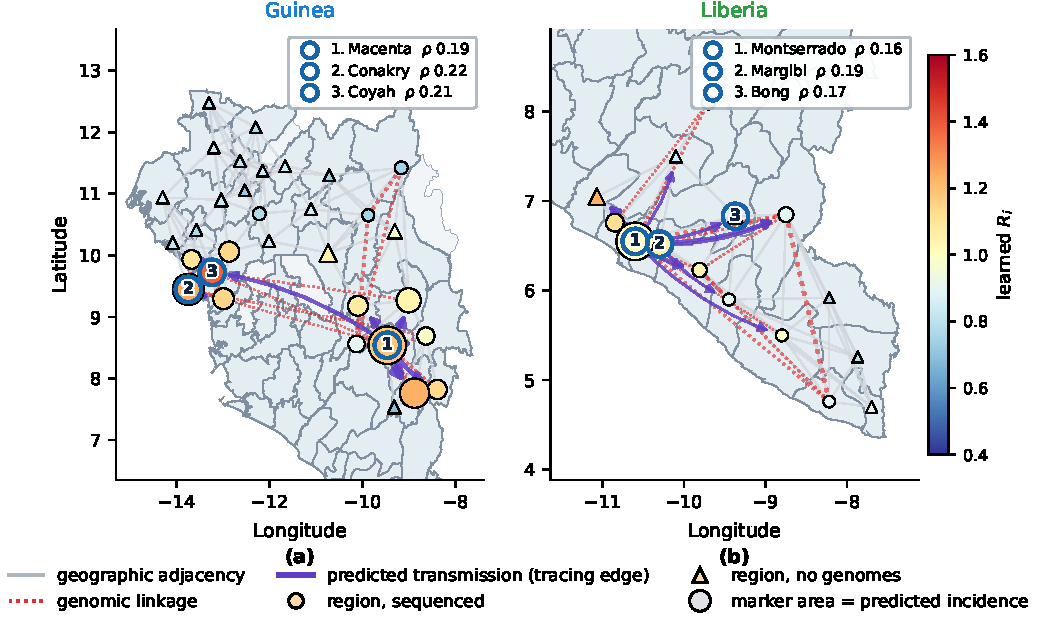
\includegraphics[width=\textwidth]{figs/tracing_a.pdf}
\caption{Predicted onward-transmission network, with the three edge types the model uses drawn over the same nodes. Grey: geographic adjacency. Red dotted: genomic transmission linkage, from genomes sampled before the forecast origin. Purple arrows: the twelve strongest predicted tracing edges $F_{i\rightarrow j}=R_j\rho_jA_{ji}P_i$, the cases the decoder expects region $j$ to import from $i$, with width proportional to weight. Marker area is predicted incidence, colour is the learned $R_i$, and triangles are regions with no sequenced cases, whose genomic row is masked. The three largest sources of onward spread are ringed and numbered, and named with their importation share $\rho_i$ in the corner key of each panel. For legibility only the eighteen strongest genomic links are drawn and node positions are relaxed by a small repulsion where seats coincide, so distances are indicative rather than exact. This is a model output, not a record of observed contacts. (a)~Guinea and (b)~Liberia; Sierra Leone and DR~Congo are in Fig.~\ref{fig:tracingb}.}
\label{fig:tracing}
\end{figure*}

\begin{figure*}[t]
\centering
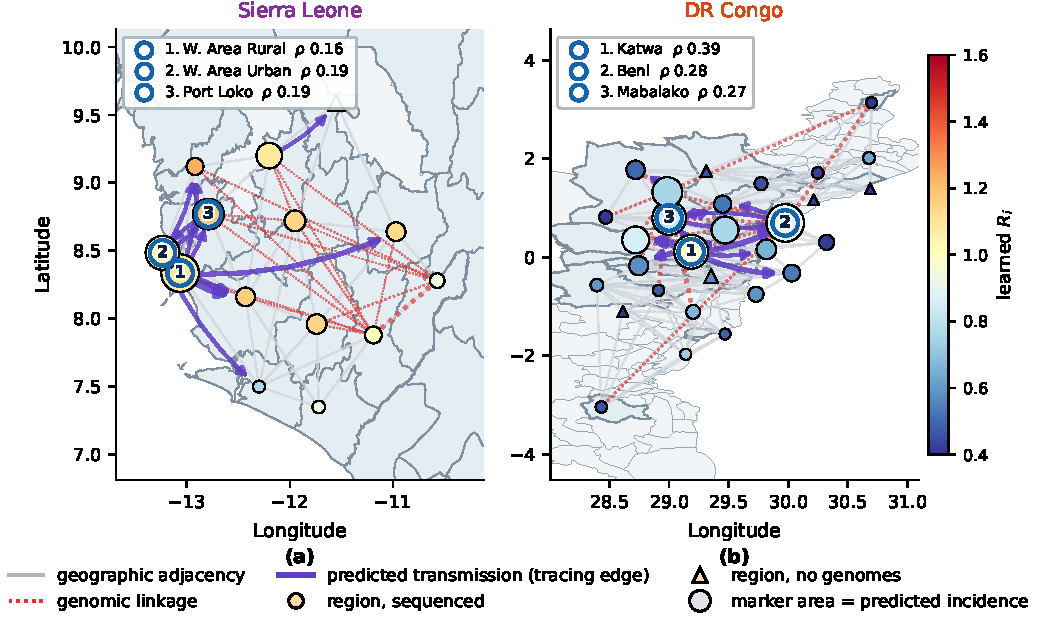
\includegraphics[width=\textwidth]{figs/tracing_b.pdf}
\caption{Predicted onward-transmission network for (a)~Sierra Leone and (b)~DR~Congo; encoding as in Fig.~\ref{fig:tracing}.}
\label{fig:tracingb}
\end{figure*}

\subsection{RQ14: where, and when, would the model send tracing teams?}

The decoder makes a statement no point forecaster can: it says how much of each region's next-week pressure is imported, and from which neighbour. Writing $F_{i\rightarrow j}=R_j\rho_jA_{ji}P_i$ for the cases region $j$ is expected to import from $i$, and accumulating $F$ over the test weeks, gives a directed network of predicted onward spread (Figs.~\ref{fig:tracing} and~\ref{fig:tracingb}). This is the quantity a tracing team prioritises on, so it is worth asking whether the model's version is sensible.

The three strongest predicted sources per country are Mac\'enta, Conakry and Coyah (Guinea); Montserrado, Margibi and Bong (Liberia); the two Western Area districts and Port Loko (Sierra Leone); and Katwa, Beni and Mabalako (DR~Congo). All twelve are documented epicentres or their immediate corridors, and the model recovers them from case counts and the genomic prior alone, with no contact data of any kind.

The networks also differ in a way that matters operationally. For the three West African countries, 32--36\% of predicted onward transmission leaves the country of origin, so a tracing programme run nationally would miss roughly a third of the expected spread. For DR~Congo the figure is zero by construction, since the panel is a single country, and the predicted flows stay inside the North Kivu corridor.


\begin{figure*}[t]
\centering
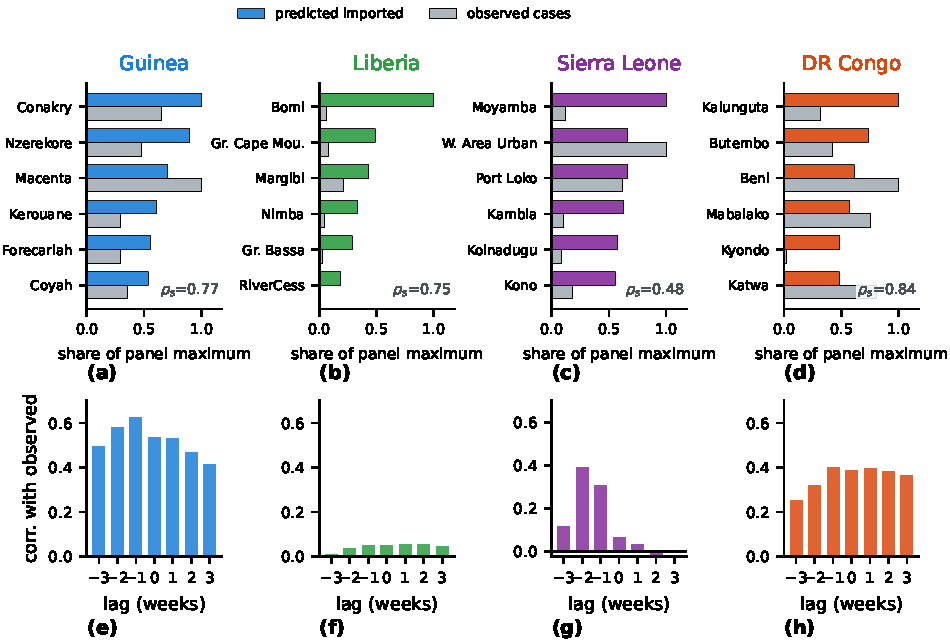
\includegraphics[width=\textwidth]{figs/tracing_time.pdf}
\caption{Tracing priority and its spatio-temporal correlation. (a)--(d)~total predicted imported cases against observed cases over the test weeks, each normalised to its panel maximum, for the six highest-pressure regions of each country; $\rho_s$ is the rank correlation between the two over all of that country's regions. There is no ground truth for \emph{imported} cases, so observed incidence is the closest available reference and the two quantities are not expected to agree. (e)--(h)~Pearson correlation between a region's predicted import pressure and its observed incidence, as a function of the lag applied to the observations on a common scale; a negative lag means the prediction leads. Guinea, Sierra Leone and DR~Congo peak at a lead of one to two weeks, while Liberia is flat at every lag.}
\label{fig:tracingtime}
\end{figure*}

The summed networks of Figs.~\ref{fig:tracing} and~\ref{fig:tracingb} hide when each link is active, so Fig.~\ref{fig:tracingtime} resolves it by week. The predicted priority is far from static: Guinea's shifts from Nz\'er\'ekor\'e and Kerouan\'e in October 2014 to Conakry and Coyah by January 2015; Sierra Leone's moves from Koinadugu and Kono through to Moyamba and the Western Area; and DR~Congo's concentrates almost entirely in a six-week burst around Katwa and Musienene in mid-2019. A team following the summed map would have been in the wrong districts for most of each outbreak.

Panel-wise, we also ask whether the predicted import pressure leads observed incidence. On Guinea the correlation peaks at a one-week lead ($r=0.62$ against $0.54$ at zero lag), on Sierra Leone at a two-week lead ($0.39$ against $0.06$), and on DR~Congo at a one-week lead ($0.40$ against $0.39$). Three of the four panels therefore place the predicted pressure ahead of the cases it is meant to anticipate, which is the ordering an operational tool needs.

Liberia is the exception and we report it as such: the correlation is essentially zero at every lag ($r\leq0.06$). This is the same panel that disagrees with the independent WHO reconstruction by 62\% (Section~\ref{sec:sources}) and on which the model performs worst at national level, so we read the flat profile as a consequence of the Montserrado backlog rather than evidence about Liberian transmission. It is also a useful negative control: the method does not manufacture a plausible-looking lead structure where the data cannot support one.

A reader may reasonably ask what the priority ranking adds over simply counting cases. Fig.~\ref{fig:tracingtime}(a)--(d) answers this directly: the rank correlation between predicted import pressure and observed incidence is 0.77 on Guinea, 0.75 on Liberia, 0.84 on DR~Congo and 0.48 on Sierra Leone. The ranking therefore tracks case volume closely on three of the four panels, and the honest reading is that most of what the tracing map says could be had from a case list. Where it differs is informative rather than noisy: Nz\'er\'ekor\'e and Coyah carry more predicted import pressure than their case counts imply, both being border districts, and the Sierra Leonean value of 0.48 reflects Moyamba and Kambia ranking far above their incidence. Those are the regions the map identifies that a case count would miss.

We state the limit of this result plainly. No contact-tracing records exist for either outbreak at this resolution, so Figs.~\ref{fig:tracing} and~\ref{fig:tracingb} cannot be validated against ground truth and we make no claim that it reproduces real transmission chains. What can be checked is that its highest-weight sources coincide with the epicentres identified retrospectively, and that its cross-border share is consistent with the genomic evidence of RQ8. It is a decision-support artefact the architecture makes available, and it should be read as a hypothesis-generating map rather than a measurement.

\section{Analysis and discussion}\label{sec:analysis}

\textbf{The advantage is concentrated, not uniform.} RQ5 (Figs.~\ref{fig:spatial} and~\ref{fig:sterr}) shows RIG-Net-GI is better on average in 79\% of DRC health zones but only 43\% of West African districts, and that its wins cluster in declining phases and secondary regions while its losses cluster in epicentres during growth and in the Montserrado backlog week; Fig.~\ref{fig:regime} localises the same split by case volume, and Table~\ref{tab:main} shows how completely pooled metrics hide it. Averaged metrics would have hidden both facts. For deployment this matters: the model is a better instrument for judging whether a chain is dying out in a secondary district than for calling the size of a surge in an epicentre.

\textbf{Where the gains come from.} Decomposing Table~\ref{tab:ablation}, the improvement from RIG-Net (15.07 WA / 1.295 DRC) to RIG-Net-GI (11.91 / 1.247): stabilisation of the rollout accounts for most of the WA gain, the genomic prior for a further 0.31 MAE there, and on DRC the ordering of the remaining components is within roughly two standard deviations, so the panels disagree about which prior matters. Priors tied to the structure of a particular outbreak help where that structure is informative, and the honest summary is that the genomic channel is valuable when cross-border introductions matter and close to inert when they do not.

\textbf{The bound explains regimes, not magnitudes.} RQ12 (Fig.~\ref{fig:theory}(c)) adds a limitation we had not previously tested: the contraction factor $\varrho(C)^3$ under-predicts realised four-week error amplification in 76\% of 195 region-blocks and does not order them correctly. The theory is therefore diagnostic, it says when the rollout is safe, but not prognostic for a given block, because the additive parameter-error term dominates in practice.

\textbf{Theory matched by experiment.} Theorem~\ref{thm:error} predicts bounded error accumulation when $\bar R<1$ and geometric growth otherwise. Both are visible in Figs.~\ref{fig:theory}(a,b),~\ref{fig:phase} and~\ref{fig:horizon}: the model is strongest in decline and tail blocks and at long horizons there, and weakest at the explosive WA peak and in the DRC growth phase. The practical implication is that a renewal decoder suits tracking an outbreak toward elimination better than calling a surge, and that a regime-aware damping of the rollout is the natural next step.

\textbf{Validation can mislead, measurably.} RQ4 (Fig.~\ref{fig:valtest}, with the fitting curves in Fig.~\ref{fig:training} and Table~\ref{tab:train}) quantifies this: validation-to-test rank correlation is 0.91 on DRC1820 but only 0.72 on WA2014, and the unpriored RIG-Net is first on validation and last on WA2014 test. Single-split studies on one outbreak are exposed to exactly this failure, and reporting the transfer correlation alongside the headline table is cheap insurance.

\textbf{Threats to validity.} Baselines are compact re-implementations with a two-point learning-rate search, while RIG-Net received a broader validation search; official implementations could rank differently. The DM test treats region--week--horizon points as independent, so overlapping horizons and spatial correlation make $p$-values anti-conservative, and ties near $p=0.05$ should be read as ties. Five seeds and 3--4 blocks per panel give 35 comparison blocks, and the Nemenyi analysis of RQ12 (Figs.~\ref{fig:cd} and~\ref{fig:variability}) shows this is still not enough to separate the leading models. Graphs use seat-town coordinates rather than boundaries or mobility data, though Table~\ref{tab:sens} shows the conclusions do not turn on how those graphs are built. Intervention indicators are surveillance-derived proxies, not intervention logs. The genomic prior is rebuilt per fold (Fig.~\ref{fig:leak}), so the leakage exposure it creates is bounded by construction rather than by assumption. The Liberian panel disagrees with an independent WHO reconstruction by 62\% in total and $r=0.20$ week to week (Fig.~\ref{fig:sources}), so Liberian results should be read with that in mind. The access indicators of Fig.~\ref{fig:nexus} are not constructed identically across countries: only Fig.~\ref{fig:nexus}(a) and~(d) use real facility data, while Fig.~\ref{fig:nexus}(b) and~(c) use a surveillance proxy, so the four should not be compared on a common scale. Genomic sampling is itself outcome-dependent (sequencing effort tracks case counts), and although~\eqref{eq:gen} normalises by $\sqrt{n_in_j}$, residual ascertainment structure may remain.

\textbf{Part of the residual error is irreducible.} Section~\ref{sec:sources} and Fig.~\ref{fig:sources}(c) measure how far two official WHO sources disagree about the same country-weeks: 142 cases for Sierra Leone and 117 for Liberia. Our national forecast errors are $1.19\times$ and $1.50\times$ those figures, so on those two panels the model is competing with the resolution of the ground truth. Reporting this changes what a further MAE gain would mean.

\textbf{Calibration is the practical dividend, with one caveat.} None of the 16 baselines emits a predictive distribution, yet an interval is what a response team acts on. The negative-binomial head needs no post-hoc calibration and is close to uniform in randomised PIT on DRC1820 (Fig.~\ref{fig:calib}, with the interval scores in Table~\ref{tab:extra}), which we regard as more useful on these data than the last few percent of MAE. On WA2014 the PIT shows over-prediction in a minority of region-weeks, so the intervals there are usable but conservative in one direction.

\textbf{What survives as interpretable.} The strongest negative result of this study is that the learned reproduction number does not reproduce an established estimator (RQ12, Fig.~\ref{fig:epiestim}). What remains usable is structural rather than inferential: the $R$ field of Fig.~\ref{fig:rfield}, the importation flows of Fig.~\ref{fig:flows}, the gate weights and suppression coefficients of Table~\ref{tab:interp}, and the per-country tracing networks of Figs.~\ref{fig:tracing},~\ref{fig:tracingb} and~\ref{fig:tracingtime}. Mechanistic structure bought us stability, phase-dependent behaviour we can predict, and a calibrated distribution; it did not by itself buy a trustworthy $R_t$. Hybrid models should be required to validate their recovered parameters against domain estimators rather than asserting interpretability from architecture.

\textbf{Surveillance breadth beats depth.} RQ10 (Figs.~\ref{fig:nexus},~\ref{fig:countries} and~\ref{fig:seq}) shows sequencing intensity and spatial coverage order the four countries differently, and it is coverage that controls how much of the genomic adjacency is usable. Liberia sequenced 1.6\% of its cases across 60\% of its counties and is where the prior helps least. For programmes deciding where to spend sequencing capacity in a future outbreak, this argues for sampling thinly across many regions rather than deeply in the epicentre, a reading the dose--response of Fig.~\ref{fig:dose} and the edge-length analysis of Fig.~\ref{fig:genval} both support.

\textbf{Future work.} Closing the gap between the learned $R$ and an epidemiological $R_t$, for example by supervising it against EpiEstim during training. Regime-switched damping of the renewal rollout; validation of the learned $R$ against EpiEstim; probabilistic scoring (weighted interval score), which the negative-binomial head supports and point baselines do not; and confirmation on held-out outbreaks such as the 2022 Uganda Sudan-virus epidemic.

\section{Conclusion}\label{sec:conclusion}

RIG-Net-GI couples a multi-graph encoder to a renewal-equation decoder carrying the Ebola generation interval, a leakage-safe genomic transmission-linkage prior and a monotone intervention-suppression term. Against 16 models published 2020--2026 under a rolling-origin protocol, it attains the lowest MAE of all systems on the DRC panel and the best RMSE, correlation and sMAPE on the West African panel while ranking fourth by MAE, and it has the best average rank over 35 dataset--fold--seed blocks. Its advantage is concentrated in declining phases, in secondary regions and at longer horizons, exactly where the theory predicts the rollout contracts, and it is weakest at explosive peaks, where the same theory predicts geometric error growth, a prediction we verify directly on the forecasts.

Three findings temper this. A Nemenyi test cannot separate RIG-Net-GI from the nine next-best models, so its first place is a ranking and not a significant win. The learned reproduction number correlates only weakly with an EpiEstim estimator and is strongly shrunk, so mechanistic structure did not by itself deliver a trustworthy $R_t$, and hybrid models should be asked to validate recovered parameters rather than assert interpretability from architecture. And the intervention component helps on one panel and not the other. What the mechanism did deliver is stability, predictable phase behaviour, calibrated predictive intervals that no point-forecasting baseline provides, and a principled slot for a genomic prior that we show carries long-range information geography cannot.

\FloatBarrier
% References for rignet.tex (43 entries, IEEE style).
% Edit entries here; the main file pulls this in with \input.
\begin{thebibliography}{99}\footnotesize\sloppy
\bibitem{agcrn} L.~Bai, L.~Yao, C.~Li, X.~Wang, and C.~Wang, ``Adaptive graph convolutional recurrent network for traffic forecasting,'' in \emph{Proc. NeurIPS}, 2020, doi:10.\allowbreak 48550/\allowbreak arXiv.\allowbreak 2007.\allowbreak 02842.\allowbreak 
\bibitem{mtgnn} Z.~Wu, S.~Pan, G.~Long, J.~Jiang, X.~Chang, and C.~Zhang, ``Connecting the dots: Multivariate time series forecasting with graph neural networks,'' in \emph{Proc. KDD}, 2020, doi:10.\allowbreak 48550/\allowbreak arXiv.\allowbreak 2005.\allowbreak 11650.\allowbreak 
\bibitem{colagnn} S.~Deng, S.~Wang, H.~Rangwala, L.~Wang, and Y.~Ning, ``Cola-GNN: Cross-location attention based graph neural networks for long-term ILI prediction,'' in \emph{Proc. CIKM}, 2020, doi:10.\allowbreak 1145/\allowbreak 3340531.\allowbreak 3411975.\allowbreak 
\bibitem{epignn} F.~Xie, Z.~Zhang, L.~Li, B.~Zhou, and Y.~Tan, ``EpiGNN: Exploring spatial transmission with graph neural network for regional epidemic forecasting,'' in \emph{Proc. ECML-PKDD}, 2022, doi:10.\allowbreak 1007/\allowbreak 978-\allowbreak 3-\allowbreak 031-\allowbreak 26422-\allowbreak 1\_29.\allowbreak 
\bibitem{staeformer} H.~Liu, Z.~Dong, R.~Jiang, J.~Deng, J.~Deng, Q.~Chen, and X.~Song, ``Spatio-temporal adaptive embedding makes vanilla transformer SOTA for traffic forecasting,'' in \emph{Proc. CIKM}, 2023, doi:10.\allowbreak 48550/\allowbreak arXiv.\allowbreak 2308.\allowbreak 10425.\allowbreak 
\bibitem{mepognn} Q.~Cao, R.~Jiang, C.~Yang, Z.~Fan, X.~Song, and R.~Shibasaki, ``MepoGNN: Metapopulation epidemic forecasting with graph neural networks,'' in \emph{Proc. ECML-PKDD}, 2022, doi:10.\allowbreak 1007/\allowbreak 978-\allowbreak 3-\allowbreak 031-\allowbreak 26422-\allowbreak 1\_28.\allowbreak 
\bibitem{stid} Z.~Shao, Z.~Zhang, F.~Wang, W.~Wei, and Y.~Xu, ``Spatial-temporal identity: A simple yet effective baseline for multivariate time series forecasting,'' in \emph{Proc. CIKM}, 2022, doi:10.\allowbreak 48550/\allowbreak arXiv.\allowbreak 2208.\allowbreak 05233.\allowbreak 
\bibitem{nbeats} B.~N. Oreshkin, D.~Carpov, N.~Chapados, and Y.~Bengio, ``N-BEATS: Neural basis expansion analysis for interpretable time series forecasting,'' in \emph{Proc. ICLR}, 2020, doi:10.\allowbreak 48550/\allowbreak arXiv.\allowbreak 1905.\allowbreak 10437.\allowbreak 
\bibitem{autoformer} H.~Wu, J.~Xu, J.~Wang, and M.~Long, ``Autoformer: Decomposition transformers with auto-correlation for long-term series forecasting,'' in \emph{Proc. NeurIPS}, 2021, doi:10.\allowbreak 48550/\allowbreak arXiv.\allowbreak 2106.\allowbreak 13008.\allowbreak 
\bibitem{dlinear} A.~Zeng, M.~Chen, L.~Zhang, and Q.~Xu, ``Are transformers effective for time series forecasting?'' in \emph{Proc. AAAI}, 2023, doi:10.\allowbreak 48550/\allowbreak arXiv.\allowbreak 2205.\allowbreak 13504.\allowbreak 
\bibitem{nhits} C.~Challu, K.~G. Olivares, B.~N. Oreshkin, F.~Garza, M.~Mergenthaler-Canseco, and A.~Dubrawski, ``N-HiTS: Neural hierarchical interpolation for time series forecasting,'' in \emph{Proc. AAAI}, 2023, doi:10.\allowbreak 48550/\allowbreak arXiv.\allowbreak 2201.\allowbreak 12886.\allowbreak 
\bibitem{patchtst} Y.~Nie, N.~H. Nguyen, P.~Sinthong, and J.~Kalagnanam, ``A time series is worth 64 words: Long-term forecasting with transformers,'' in \emph{Proc. ICLR}, 2023, doi:10.\allowbreak 48550/\allowbreak arXiv.\allowbreak 2211.\allowbreak 14730.\allowbreak 
\bibitem{timesnet} H.~Wu, T.~Hu, Y.~Liu, H.~Zhou, J.~Wang, and M.~Long, ``TimesNet: Temporal 2D-variation modeling for general time series analysis,'' in \emph{Proc. ICLR}, 2023, doi:10.\allowbreak 48550/\allowbreak arXiv.\allowbreak 2210.\allowbreak 02186.\allowbreak 
\bibitem{tsmixer} S.-A. Chen, C.-L. Li, N.~Yoder, S.~O. Arik, and T.~Pfister, ``TSMixer: An all-MLP architecture for time series forecasting,'' \emph{TMLR}, 2023, doi:10.\allowbreak 48550/\allowbreak arXiv.\allowbreak 2303.\allowbreak 06053.\allowbreak 
\bibitem{mastnet} A.~J. Fofanah, L.~Wen, and D.~Chen, ``MAST-Net: Manifold-constrained adaptive spatio-temporal network for traffic flow forecasting,'' \emph{J. Netw. Comput. Appl.}, 2026, doi:10.\allowbreak 1016/\allowbreak j.\allowbreak jnca.\allowbreak 2026.\allowbreak 104543.\allowbreak 

\bibitem{chamformer} A.~J. Fofanah, D.~Chen, L.~Wen, and S.~Zhang, ``CHAMFormer: Dual heterogeneous three-stages coupling and multivariate feature-aware learning network for traffic flow forecasting,'' \emph{Expert Systems with Applications}, vol. 266, p. 126085, 2025, doi:10.\allowbreak 1016/\allowbreak j.\allowbreak eswa.\allowbreak 2024.\allowbreak 126085.\allowbreak 
\bibitem{deepevd} A.~J. Fofanah, A.~A. Kamara, A.~P. Sankoh, T.~Gao, I.~Dumbuya, and Z.~B. Conteh, ``DeepEVD: Integrating epidemiological data into deep learning frameworks based on spatio-temporal feature learning for EVD forecasting,'' \emph{Spatial and Spatio-temporal Epidemiology}, p. 100741, 2025, doi:10.\allowbreak 1016/\allowbreak j.\allowbreak sste.\allowbreak 2025.\allowbreak 100741.\allowbreak 
\bibitem{stflam} A.~J. Fofanah, A.~P. Sankoh, I.~Dumbuya, A.~A. Kamara, and Z.~B. Conteh, ``ST-FLAM: Evaluating performance of deep learning models on mobility patterns for EVD forecasting based on spatio-temporal feature learning,'' in \emph{Proc. 13th Int. Conf. Networks, Communication and Computing (ICNCC)}, 2024, pp. 98--106, doi:10.\allowbreak 1145/\allowbreak 3711650.\allowbreak 3711665.\allowbreak 
\bibitem{mcpst} A.~J. Fofanah, L.~Wen, and D.~Chen, ``MCPST: A multi-phase consensus and spatio-temporal learning for few-shot traffic forecasting via physical dynamics,'' \emph{IEEE Internet of Things Journal}, 2026, doi:10.\allowbreak 1109/\allowbreak JIOT.\allowbreak 2026.\allowbreak 3700641.\allowbreak 

\bibitem{xcity} A.~J. Fofanah \emph{et al.}, ``Spatio-temporal feature fusion and few-shot learning framework with cross-city knowledge transfer for traffic flow prediction,'' \emph{Energy and AI}, 2026, doi:10.\allowbreak 1016/\allowbreak j.\allowbreak egyai.\allowbreak 2026.\allowbreak 100797.\allowbreak 
\bibitem{cl3an} A.~J. Fofanah \emph{et al.}, ``CL3AN-GNN: Curriculum-driven incremental feature disentanglement with multi-phase attention for class-imbalanced node classification,'' \emph{Neural Computing and Applications}, 2026, doi:10.\allowbreak 1007/\allowbreak s00521-\allowbreak 026-\allowbreak 12579-\allowbreak x.\allowbreak 
\bibitem{legrand2007} J.~Legrand, R.~F. Grais, P.-Y. Boelle, A.-J. Valleron, and A.~Flahault, ``Understanding the dynamics of Ebola epidemics,'' \emph{Epidemiology \& Infection}, vol. 135, no. 4, pp. 610--621, 2007, doi:10.\allowbreak 1017/\allowbreak S0950268806007217.\allowbreak 
\bibitem{rojek2025} A.~Rojek \emph{et al.}, ``Ebola disease: Bridging scientific discoveries and clinical application,'' \emph{The Lancet Infectious Diseases}, vol. 25, no. 3, pp. e165--e176, 2025, doi:10.\allowbreak 1016/\allowbreak S1473-\allowbreak 3099(24)00673-\allowbreak X.\allowbreak 
\bibitem{yunus2025} A.~O. Yunus and M.~O. Olayiwola, ``Dynamics of Ebola virus transmission with vaccination control using Caputo--Fabrizio fractional-order derivative analysis,'' \emph{Modeling Earth Systems and Environment}, vol. 11, no. 3, p. 175, 2025.
\bibitem{memilio2026} J.~Bicker \emph{et al.}, ``MEmilio: A high performance modular epidemics simulation software for multi-scale and comparative simulations of infectious disease dynamics,'' \emph{Scientific Reports}, vol. 16, no. 1, p. 26950, 2026.
\bibitem{sun2026} G.-Q. Sun, L.-F. Hou, X.~Luo, Q.-H. Liu, and X.~Lu, ``Spatiotemporal dynamics of infectious diseases: From mechanistic models to data-driven models,'' \emph{Journal of Data and Dynamic Systems}, vol. 2, pp. 19--78, 2026.
\bibitem{zhang2026} Y.~Zhang \emph{et al.}, ``A scoping review of machine learning applications across epidemiological stages of zoonotic disease,'' \emph{Transboundary and Emerging Diseases}, vol. 2026, no. 1, p. 2215823, 2026.
\bibitem{liu2023human} Y.~Liu, Y.~Rong, Z.~Guo, N.~Chen, T.~Xu, F.~Tsung, and J.~Li, ``Human mobility modeling during the COVID-19 pandemic via deep graph diffusion infomax,'' in \emph{Proc. AAAI}, vol. 37, no. 12, 2023, pp. 14{,}347--14{,}355, doi:10.\allowbreak 1609/\allowbreak aaai.\allowbreak v37i12.\allowbreak 26678.\allowbreak 
\bibitem{quick2016} J.~Quick \emph{et al.}, ``Real-time, portable genome sequencing for Ebola surveillance,'' \emph{Nature}, vol. 530, no. 7589, pp. 228--232, 2016, doi:10.1038/nature16996.
\bibitem{grubaugh2019} N.~D. Grubaugh \emph{et al.}, ``Tracking virus outbreaks in the twenty-first century,'' \emph{Nature Microbiology}, vol. 4, no. 1, pp. 10--19, 2019, doi:10.1038/s41564-018-0296-2.
\bibitem{hadfield2018} J.~Hadfield \emph{et al.}, ``Nextstrain: Real-time tracking of pathogen evolution,'' \emph{Bioinformatics}, vol. 34, no. 23, pp. 4121--4123, 2018, doi:10.1093/bioinformatics/bty407.
\bibitem{bracher2021} J.~Bracher, E.~L. Ray, T.~Gneiting, and N.~G. Reich, ``Evaluating epidemic forecasts in an interval format,'' \emph{PLoS Computational Biology}, vol. 17, no. 2, e1008618, 2021, doi:10.1371/journal.pcbi.1008618.
\bibitem{cramer2022} E.~Y. Cramer \emph{et al.}, ``Evaluation of individual and ensemble probabilistic forecasts of COVID-19 mortality in the United States,'' \emph{Proceedings of the National Academy of Sciences}, vol. 119, no. 15, e2113561119, 2022, doi:10.1073/pnas.2113561119.
\bibitem{diebold1995} F.~X. Diebold and R.~S. Mariano, ``Comparing predictive accuracy,'' \emph{Journal of Business \& Economic Statistics}, vol. 13, no. 3, pp. 253--263, 1995, doi:10.1080/07350015.1995.10524599.
\bibitem{itransformer} Y.~Liu, T.~Hu, H.~Zhang, H.~Wu, S.~Wang, L.~Ma, and M.~Long, ``iTransformer: Inverted transformers are effective for time series forecasting,'' in \emph{Proc. ICLR}, 2024, doi:10.\allowbreak 48550/\allowbreak arXiv.\allowbreak 2310.\allowbreak 06625.\allowbreak 
\bibitem{who2014} WHO Ebola Response Team, ``Ebola virus disease in West Africa, the first 9 months of the epidemic and forward projections,'' \emph{New England Journal of Medicine}, vol. 371, no. 16, pp. 1481--1495, 2014, doi:10.\allowbreak 1056/\allowbreak NEJMoa1411100.\allowbreak 
\bibitem{dudas2017} G.~Dudas \emph{et al.}, ``Virus genomes reveal factors that spread and sustained the Ebola epidemic,'' \emph{Nature}, vol. 544, pp. 309--315, 2017, doi:10.\allowbreak 1038/\allowbreak nature22040.\allowbreak 
\bibitem{kinganda2021} E.~Kinganda-Lusamaki \emph{et al.}, ``Integration of genomic sequencing into the response to the Ebola virus outbreak in Nord Kivu, Democratic Republic of the Congo,'' \emph{Nature Medicine}, vol. 27, pp. 710--716, 2021, doi:10.\allowbreak 1038/\allowbreak s41591-\allowbreak 021-\allowbreak 01302-\allowbreak z.\allowbreak 
\bibitem{cori2013} A.~Cori, N.~M. Ferguson, C.~Fraser, and S.~Cauchemez, ``A new framework and software to estimate time-varying reproduction numbers during epidemics,'' \emph{American Journal of Epidemiology}, vol. 178, no. 9, pp. 1505--1512, 2013, doi:10.\allowbreak 1093/\allowbreak aje/\allowbreak kwt133.\allowbreak 
\bibitem{fraser2007} C.~Fraser, ``Estimating individual and household reproduction numbers in an emerging epidemic,'' \emph{PLoS ONE}, vol. 2, no. 8, e758, 2007, doi:10.\allowbreak 1371/\allowbreak journal.\allowbreak pone.\allowbreak 0000758.\allowbreak 
\bibitem{riley2007} S.~Riley, ``Large-scale spatial-transmission models of infectious disease,'' \emph{Science}, vol. 316, no. 5829, pp. 1298--1301, 2007, doi:10.\allowbreak 1126/\allowbreak science.\allowbreak 1134695.\allowbreak 
\bibitem{hyndman2006} R.~J. Hyndman and A.~B. Koehler, ``Another look at measures of forecast accuracy,'' \emph{International Journal of Forecasting}, vol. 22, no. 4, pp. 679--688, 2006, doi:10.1016/j.ijforecast.2006.03.001.
\bibitem{gneiting2011} T.~Gneiting, ``Making and evaluating point forecasts,'' \emph{Journal of the American Statistical Association}, vol. 106, no. 494, pp. 746--762, 2011, doi:10.\allowbreak 1198/\allowbreak jasa.\allowbreak 2011.\allowbreak r10138.\allowbreak 
\end{thebibliography}


\end{document}
